\documentclass[letterpaper,twocolumn,10pt]{article}
\usepackage{usenix2019_v3}
\usepackage{preamble}


% to be able to draw some self-contained figs
\usepackage{tikz}
\usepackage{amsmath}
\usepackage{xspace}
% inlined bib file
\usepackage{filecontents}
\usepackage{algorithm}
\usepackage{amsthm}
\usepackage[noend]{algpseudocode}
\usepackage{mathtools}
%\usepackage[ruled, vlined, linesnumbered]{algorithm2e}
\usepackage{mdframed}
\usepackage{enumitem}
\usepackage{xcolor}
\setlist{itemsep=0pt,parsep=0pt}             % more compact lists
\usepackage[belowskip=-15pt,aboveskip=5pt]{caption}
 
%\setlength{\intextsep}{10pt plus 2pt minus 2pt}
%-------------------------------------------------------------------------------
\begin{document}
%-------------------------------------------------------------------------------

%don't want date printed
\date{}

% make title bold and 14 pt font (Latex default is non-bold, 16 pt)
\title{\Large \bf Indicus: Unchaining Byzantine Databases\\
 }

%for single author (just remove % characters)
\author{
{\rm Your N.\ Here}\\
Your Institution
\and
{\rm Second Name}\\
Second Institution
% copy the following lines to add more authors
% \and
% {\rm Name}\\
%Name Institution
} % end author

\maketitle

%-------------------------------------------------------------------------------
\begin{abstract}
%-------------------------------------------------------------------------------
Your abstract text goes here. Just a few facts. Whet our appetites.
Not more than 200 words, if possible, and preferably closer to 150.
\end{abstract}


%-------------------------------------------------------------------------------
\section{Introduction} 
%-------------------------------------------------------------------------------

%


This paper introduces Indicus, the first leaderless transactional key-value store that is robust in the Byzantine Fault Model. Indicus aims to mitigate the tension between real-world, highly commutative transaction workloads striving for scalability, and the simplicity that totally ordered ledger abstractions such as Blockchains or State Machine Replication offer.

\fs{this maybe sounds too much like a permissioneless blockchain} Specifically, this paper asks the question: how can we enable \textit{mutually distrustful parties} to consistently, reliably share and scalably share data, while minimizing centralization. \\


The ability to share data online offers exciting opportunities; however, increased datasharing also raises the concern of how to \textit{decentralize trust}. In banking, systems like SWIFT (cite) enable financial institutions to quickly and accurately enable cross-institutional transaction clearance, at the cost of placing their trust in the centralized SWIFT network. In manufacturing, online data sharing can improve accountability and auditing amongst the globally distributed supply chain, but there may not be an identifiable source of trust. Consider the supply chain for the latest iPhone: it spans three continents, and hundreds of different contractors \cite{AppleSup} that may neither trust Apple, nor each other, yet must be willing to share and agree on information concerning the construction of the same product. Even sole entities that distribute their dataceneters globally (i.e. Google, Amazon), may not trust their \textit{own} datacenters located in authoritative domains or legislations out of its control.\\


Recognizing this challenge by both the research and industrial communities, much effort has focused on enabling shared computation \fs{sounds like we will talk about secure Multi party computation} between mutually distrustful parties in the context of Byzantine Fault Tolerance (BFT) and Blockchains. 
Systems proposed in the literature of BFT provide the abstraction of a totally ordered request log; the log is agreed upon by the \textit{n} participants in the system, of which at most \textit{f} can misbehave. In the Blockchain world, Bitcoin and Ethereum have become popular distributed computing platforms providing the same log abstraction while aiming for decentralizing trust and open membership \fs{at much lower throughput, more power consumption, no finality}. At the intersection, systems such as Hyperledger Fabric \cite{Hyperledger} or Ethereum Quorum \cite{EthereumQuorum} aim to cater to Blockchain markets while leveraging traditional BFT approaches for scalability. Efforts to incorporate Blockchain/BFT technologies into market ready infrastructures are pervasive \cite{StateFarmQuorum, AutoInventory, StateFarmQuorum2, HyperledgerTelecom, HyperledgerHealth}. \\



In this paper however, we argue that existing solutions merely shoehorn the desired functionality of transactional applications rather than catering to the principal requirements. 
\fs{Hyperledger itself claims to be a shared database}
While applications in stronger failure domains \fs{(Crash Failure)} are built atop transactional Databases whose primary design concern is performance, applications in Byzantine Failure assumptions must resort to systems designed instead for fault tolerance as primary design concern and scalability as optimization concern. Instead, we argue, that the sustainable way to service applications requiring BFT is to build dedicated databases that are co-designed with byzantine resilience. \fs{people might disagree}
Concretely, we stipulate that an appropriate Database for the Byzantine Fault Model should 1) maintain the \textit{abstraction} of a sequential execution, 2) be scalable, 3) be resitant to censorship and frontrunning and 4) bound the effects of byzantine components, be it replicas or clients.
We outline how existing approaches fall short of satisfying one or more of these requirements, and finally propose a system to fill this gap.

\fs{paragraphs of shortcomings cut here and moved to section 2 in extended form.}
\iffalse
\fs{CUT from HERE}
First, we argue there exists a fundamental mismatch between the implementation of a totally ordered log and the reality of much large-scale distrubted processing. Many large-scale distributed systems consists primarily of unordered and unrelated operations. For example, a product supply chain consists of many concurrent steps that do not require ordering. Imposing an ordering on non-conflicting operations is not only often unecessary, but costly: participants in the shared computation must vote to order operations and serialize request execution accordingly, thus harming both throughput and end-to-end latency. \fs{people can claim that there exist partially ordered solutions -> Dag blockchains, clairvoyant}\\

Second, while there exists work on mitigating this scalability bottleneck through sharding (cite Omniledger, Chainspace, Callinicos), it remains largely an engineering optimization. At its core, the application of sharding conflates two objectives: Horizontal hardware scaling and transactional concurrency \fs{too vague currently}. When a mapping from data to shards is well chosen (note, that this relies on application specific knowledge) partial ordering between objects on different shards manifests as a side-effect of seperating resources \fs{will others agree to this view?}. In fact, when transactions span multiple shards, the latent total order requirement can introduce redundant coordination overheads, as coordination may need to be performed twice, at the level of individual shards, and across shards \cite{zhang2016operation}. This is especially problematic when workloads are geo-replicated (citation?), or when, as in BFT, the replication factor is high \fs{why? be more specific}. \\

Third, achieving a total order often \fs{What if not? OR: Is it even possible without leader?} necessitates a single point of centralization, in order to propose a sequencing order. This is especially undesirable in trust concerned settings as such a sequencer exposes not only a scalability bottleneck but a fairness vulnerability. A sequencer may be biased, frontrun requests or censor others and is inherently antithetical to the need of decentralized, trustless solutions.\\

Lastly, most BFT/Blockchain systems support transactions under the assumption that their read and write operations are known a priori, which limits the set of applications that they can support. \fs{this is sort of random and not in line with the requirements above}


In summary, prior BFT solutions succumb to one or more of the following fallacies, some of which are correlated: They a) impose a restrictive total order, b) use leader in some form or another, c) assume fixed transaction sets or d) incur redundant coordination overheads when sharding. \\

\fs{this paragraph feels like taking a step back}
Leveraging commutativity between transactions is not a new idea. As a research trend of mitigating the scalability bottleneck, EPaxos (cite), TAPIR (cite) and CURP (cite) only consider the ordering between potentially conflicting operations. However, these systems assume the stronger crash-failure model and are non-trivial to extend to the Byzantine model, so that they cannot directly solve the problem of data sharing among mutually distrustful, malicious or arbitrarily failing parties.
\fs{CUT TILL HERE}
\fi

Existing research, in essence, is either attempting to build concurrency control and sharding functionalities over BFT replication, or integrating these functionalities into a crash-failure replication protocol. In this paper, we will show how to build these desiring functionalities inside a BFT replication protocol. Specifically, our goal is to \textit{provide the illusion of a centralized shared log, rather than the non-scalable reality of a totally ordered log}.\\

\fs{paragraph on CF systems cut and moved to section 2}
\iffalse
\fs{rambling too long}
\fs{CUT FROM HERE}

While copious efforts exist to design decentralized systems that exploit transaction semantics for the crash failure model, few, if any attempts have been made for the Byzantine Fault Model. This naturally raises the question, why so? One explanation is that in Byzantine Systems, some centralization is in fact highly desirable as it simplifies the problem by identifying a single point of accountability. A natural way to improve both scalability and fairness is to avoid this bottleneck, at the cost of paving the path for a wider set of undesirable phenomena. The challenge of a leaderless byzantine system is simple yet daunting: It empowers both malicious users and system components to collude and misbehave in potentially unaccountable ways.
In this paper we will show to overcome this challenge by designing and implementing the leaderless BFT system Indicus that avoids near-all centralization while replicating interactive ACID transactions in a partial order. 
\fs{client driven protocol could be seen as nightmare for byz system. What is our design agenda to control this? -> Byz can only influence itself. Honest users can keep using the system }\\
\fs{CUT TILL HERE}
\fi

In this paper we will show to realize this goal by designing and implementing a leaderless BFT database system called Indicus, that avoids near-all centralization while replicating interactive ACID transactions in a partial order. Distinctively, Indicus does not aim to be the 701th BFT State Machine Replication protocol (cite the next 700 bft), but the first BFT protocol to integrate replication and transaction layer.

Indicus' design is driven by the ethos of \textit{independent operability}; both safety \fs{(integrity, serializability)} and liveness \fs{ability to issue and complete TX} are per-client properties and independent from one client to another.
\fs{Indicus embraces partial order across the entire transaction stack} Unlike State Machine Replication (SMR) based systems that achieve agreement on computation (i.e. state transitions) by imposing a total order on execution across all replicas, Indicus executes transactions speculatively at clients, while validating and replicating \textit{all} transactions in arbitrary order at any given replica. Furthermore, clients coordinate the agreement protocol themselves, thus putting them in charge of their own transactions. Doing so, while tolerating byzantine client behavior, is Indicus' main challenge; In Indicus \textit{the client is king - but rulers have to be regulated}.

Abstractly, Indicus proposes each transaction for a seperate concurrent binary consensus instance and enforces an implicit partial order by aborting transactions when inconistencies arise. In order to maintain a serializable transaction history, Indicus assigns each transaction an optimistic timestamp and uses a variation of Multiversioned Timestamp Ordering (MVTSO) for concurrency control. Ordering conflicts between transactions whose interleavings would violate prescribed Isolation guarantees are broken based on the given timestamps and speculative execution results. \fs{does all of this need to be in an intro? There needs to be a little of key insight, but it feels more appropriate for discussion}\\



Overall, the Indicus design has the following implications:
\begin{itemize}%[noitemsep,topsep=0pt,parsep=0pt,partopsep=0pt]

\item Indicus is robust to censorship and frontrunning as there exist no central authority that admits and orders transactions.
\item Indicus allows commutative/non-conflicting Transactions to both be executed and validated out of order, thus maximizing parallelism. \fs{ (This should increase throughput and reduce latency, because clients arent waiting for all previously sequenced tx to finish. Consequently the tail latency does not dominate throughput as much.)}
\item Indicus minimizes the state, communication and computation load on replicas, as Clients serve as both execution hub and broadcast channel for their own Transactions. \fs{optional:}(This avoids quadratic communication communication complexity in the normal case.) \fs{(Theoretically always, but we keep some for practicality in the fallback)}
\item As any Quorum system, Indicus is inherently load-balanced as there exists no leader bottleneck and all replicas share equal responsibilities.
\item In Indicus liveness is a client local property. Unlike common SMR protocols, where the entire system halts during view changes, Byzantine participants may stall system progress only for the objects their transactions touch. Hence, the system appears live to any non-conflicting Transaction.
\end{itemize}

To achieve these properties Indicus incurs two main tradeoffs. First, shifting responsibility from replicas to clients comes at the cost of higher computational requirements for clients, which may not be tolerable for all applications. In practice we envision Indicus clients to be dedicated transaction managers, rather than end users. Second, like all optimistic concurrency control schemes, Indicus is vulnerable to congestion. When contention is high, abort rate soars; Indicus is not designed for such applications. Exploring tradeoffs between client/replica responsibilities as well as pessimistic concurrency control mechanisms are potential avenues for future work.

Results:  ...

To summarize, this paper makes three main contributions:
\begin{enumerate}
\item It offers definitions for transactional Isolation guarantees for the Byzantine Fault Model
\item It presents the design, implementation, and evaluation of the first leaderless ACID transactional system that tolerates Byzantine Failures
\item It presents two variations (Indicus3 and Indicus5) of a client centric agreement mechanism that trade-off performance for replication degree.  
\item \fs{our MVTSO?}
\end{enumerate}

\fs{perhaps unecessary}
The rest of the paper is structured as follows. In section 2 we elaborate the shortcomings of existing systems and challenges that the proposed design faces. In section 3 we delineate the system model and offer general purpose definitions for reasoning about byzantine databases. In section 4 and 5 we outline the Indicus architecture and protocols respectively. Section 6 describes our evaluation, while section 7 discusses limitations of the Indicus design. Finally, section 7 concludes the paper. 

\iffalse
Please check these links from the ref.bib yourself. Most of them are internet pages. (some only secondary sources, i.e. articles, so they may be useless). Some whitepapers\\
Health: \cite{HyperledgerHealth}\\
Insurance Services \cite{StateFarmSubrogation}   secondary sources: \cite{StateFarmQuorum, StateFarmQuorum2}\\
Financial: \cite{IBMSettlements, Libra}\\
Supply Chain:  \cite{IBMFoodSupply, DeloitteSupply}   secondary sources: \cite{SupplyExamples,}\\
Other:  \cite{HyperledgerTelecom}  secondary sources: \cite{AutoInventory}\\
\fi


This paper presents the design and evaluation of \sys{}, the first leaderless and scalable transactional key-value store that is robust to Byzantine faults.

Safe and efficient online data sharing among mutually distrustful
parties offers exciting opportunities for a variety of applications,
including healthcare~\cite{HyperledgerHealth}, financial services~\cite{IBMSettlements, Libra, StateFarmSubrogation}, supply chain
management~\cite{IBMFoodSupply, DeloitteSupply} and more~\cite{HyperledgerTelecom}. Consider the supply chain for the latest iPhone: it spans three continents, and hundreds of different contractors \cite{AppleSup} that may neither trust Apple, nor each other, yet must be willing to share and agree on information concerning the construction of the same product.
Byzantine fault tolerant (BFT)
systems~\cite{castro1999practical,martin2006fast,kotla2007zyzzyva,  gueta2018sbft,clement2009making,buchman2016tendermint,yin2019hotstuff,Clement09Upright,duan2014hbft, pires2018generalized,bessani2014state,lamport2011byzantizing,arun2019ezbft, malkhi2019flexible,duan2014hbft,yin2003separating, Guerraoui08Next, Kotla04High,liskov2010viewstamped} and permissioned blockchains~\cite{Hyperledger,EthereumQuorum, buchman2016tendermint, al2017chainspace,kokoris2018omniledger,gilad2017algorand, baudet2019state} are at the center of these new services. These protocols are guaranteed to
produce the same totally ordered log of operations across mutually distrustful
participants. 

The abstraction of a totally ordered log of operations is appealing simple. {\em Implementing} a totally ordered log, however, is hard to scale, as sequencing all requests can become a bottleneck \fs{sentence does not quite sound right: Implementations are hare to scale, "implementing" is not}. Fortunately, a total order is  often unnecessary, as most distributed applications primarily consist of independent and logically concurrent operations. Supply chains for instance, despite their name, are actually complex networks that generate and process logically concurrent transactions. 

Some BFT systems attempt to tap this opportunity for greater parallelism by leveraging sharding: operations within each shard continue to be totally ordered, but transactions that involve operations in disjoint (subsets of) shards can execute concurrently. Transactions involving  multiple shards are executed by running cross-shard atomic commit protocols that leverage the intra-shard total order of operations \cite{kokoris2018omniledger, al2017chainspace, zamani2018rapidchain, padilha2016callinicos}. 

These designs have several known drawbacks: \one~ they pay the performance penalty of  redundant coordination---both across shards (to commit distributed transactions) and among the replicas within each shard (to enforce total order)~\cite{zhang2016operation, zhang2015tapir, mu2016consolidating}; \two~within each shard,  they give to a leader disproportionate influence over the specific total order that is ultimately agreed upon: this has recently raised fairness concerns in the context of blockchains~\cite{herlihy2016enhancing, yin2019hotstuff}; and they restrict the expressiveness of the transactions they support~\cite{padilha2016callinicos}. \fs{the limited tx model is still kind of disjoint}

\changebars{}{Even more fundamentally, however, they are inherently limited in the concurrency  they can achieve, since, within each shard,  they continue to totally order logically concurrent operations. Sharding is simply too coarse a mechanism and its effectiveness too workload-dependent to fully expose parallelism.} \fs{do not like this sentence currently}
\nc{i think this paragraph is confusing and could be removed completely}

In this paper we advocate a more principled approach to support the abstraction of a totally ordered log \changebars{that expressingly exploits workloads' inherent parallelism}{while aggressively pursuing concurrency in its implementation}. In particular, we  make our own the lesson of distributed databases \fs{sounds a little odd to me, but I get the point}. These systems have long recognized that it is not necessary to implement a total order of transactions to offer the abstraction of a serializable execution: serializability, the gold-standard database criterion, defines a correct execution as one that is \textit{equivalent} to a serial schedule ~\cite{bernstein1979fas,Papadimitriou1979serializability,bernstein1979fas}.  This definition allows concurrent operations to execute in parallel and orders conflicting operations only.  We submit that Byzantine systems need be no different. This paper consequently argues for a paradigm "flip": rather that building a BFT data-sharing systems by layering database-like transactions and sharding on top of a BFT log, we  build out the abstraction of a BFT log atop a partially ordered distributed database.



\iffalse

% Existing research attempts to mitigate the aforementioned scalability bottleneck through a combination of sharding \changebars{and cross-shard atomic commit protocols, which they layer atop the totally ordered requests}{, cross-shard atomic commit protocols and centralised ordering services}~\cite{kokoris2018omniledger,al2017chainspace,padilha2016callinicos}. These systems suffer from three primary drawbacks \one ~ they limit the expressivity of the transactions they support \two ~ they introduce unnecessary coordination across replicas and finally, \three ~ they often centralise the ordering of requests at a single leader, which raises fairness \fs{and scalability - cyclic mention.. - instead single point of failure?} concerns. These limitations all stem from the same fallacy: the mistaken belief that building out a total order of operations is necessary for correctness.  \fs{these limitations currently don't read as if they are intertwined - when I think they should. I.e. the transaction expressiveness is limited in order to make the other limitations more scalable} \fs{transaction limited expressiveness only partially attributtable to total order imo - ; ALSO: the 2 blockchain citations use the UTXO model, its probably a stretch to say that has to due with totally ordered based? Even with partial order one-shot models are desirable (UTXO is a oneshot in my eyes), since thats single round communication/coordination}


\fs{people have been building the abstraction of a total order on top of a physical total order, i.e. the implementation mirrors abstraction. They KNOW that total order is limiting, its not a new idea or mistaken belief. The question is, whether it is possible to do it differently - we want to instead provide a different implementation. And people HAVE tried: But only for crash failure - or, only via sharding }

\fs{alternative version in comments}
\fi
\iffalse
Maintaining a totally ordered log of requests, despite its appealing simplicity, is problematic:
Such an approach is hard to scale \changebars{and costly to implement} as all agreement instances must be serialized, which in turn is often enforced by a dedicated sequencer, thus exposing both a throughput bottleneck and a single point of failure \fs{citation? Epaxos, BFT Mir: says leader is network bottleneck}. This total order is in fact often unnecessary; modern distributed applications primarily consist of independent operations that could be executed concurrently. Supply chains for instance, despite their name, are actually complex networks that generate and process logically concurrent transactions. \fs{2nd mention of supply chains as example already}
While this observation is frequently leveraged by distributed transaction protocols in the crash-fault model \cite{a bunch}, it has found scarce \cite{Clairvoyant} attention in the BFT space \fs{could we add a sentence for why? i.e. the simplicity of total order is so tempting?}.

Instead, existing research attempts to mitigate the aforementioned scalability bottleneck through the application of sharding and cross-shard atomic commit protocols on top of centralised ordering services~\cite{kokoris2018omniledger,al2017chainspace,padilha2016callinicos}. The application of sharding however, conflates the functionality of horizontal scalability with the objective of a partial-order and remains an engineering optimization dependent on workload-specific partition mappings.
On a high level, existing systems suffer from three primary drawbacks \one ~ they limit the expressivity of the transactions they support \fs{the above citations refer to UTXO models, bad comparison; I figure this is supposed to refer to things like Callinicos} \two ~ they introduce unnecessary coordination across replicas and finally,
\three ~ they often centralise the ordering of requests at a single leader, which, in addition to bottleneck concerns, raises fairness concerns for BFT settings. These limitations all stem from the same fallacy: the mistaken belief that building out a total order of operations is necessary for correctness. 
\fi



\iffalse 
In reality, building \textit{the abstraction} of a total order is sufficient, and distributed databases have long recognised this fact~\cite{crooks2018obladi,bernstein1979fas,Papadimitriou1979serializability,adya99weakconsis}. \fs{at this point a reader could expect us to talk about partial order and sharding - if we cut the Background section we currently do not mention sharding anywhere. That could seem ignorant.} Serializability, the gold-standard database criterion, defines a correct execution as one that is \textit{equivalent} to a correct schedule~\cite{bernstein1979fas,Papadimitriou1979serializability,bernstein1979fas}. This definition allows concurrent operations to execute in parallel and orders conflicting operations only.  Byzantine systems need be no different. This paper consequently argues for a paradigm "flip". The
right way to build BFT data-sharing systems is not to layer database-like transactions and sharding on top of a BFT log, but instead to do the opposite and build out the abstraction of a BFT log atop a partially ordered distributed database.
\fi
To this effect, we design \sys{}, the first leaderless and scalable key-value store that is resilient against
Byzantine faults, and specifically formalize the notion of \textit{Byzantine isolation}, the correctness
guarantee that any BFT distributed database should enforce.  \sys{} provides three main benefits.

 First, it overcomes the scalability bottleneck of a low-level
implementation based on a totally ordered BFT log. \sys instead leverages databases' ability to support highly concurrent transaction
processing while maintaining the abstraction
of a serial execution.

% an explicit ordering service 

Second, by doing away with an underlying totally ordered log, \sys{} can
sidestep the growing concerns~\cite{} about whether blockchains
order transactions fairly. Though the notion of fairness in this
context has not been rigorously defined, leaving the ordering to the
whim of a potentially Byzantine leader, as some protocols do~\cite{
Kotla07Zyzzyva,castro1999practical}
is intuitively problematic \cite{herlihy2016enhancing}. In contrast, \sys leaves the
responsibility of driving the replication and distributed commit of a
transaction to the client that proposes it \changebars{fs: cut imo}{and allows separate 
shards to order transactions independently as the total order abstraction afforded by Byzantine serializability can be maintained. } \fs{Limitation of client computation can come here: "A cost in doing so is higher computational load for clients"}

Third, \sys{} avoids the duplicate ordering costs of transactional systems
built on top of state machine replication. As Tapir noted~\cite{zhang2015tapir,mu2016consolidating},
these systems require a consistent ordering of
operations within each shard for replication, and additionally enforce a serial order of transactions across
shards for distributed commit. In contrast, \sys{} integrates distributed commit with 
replication and
limits coordination to the validation step of the distributed commit
protocol. %\fs{mention the shortcoming of using sharding for PO here}

In practice, reaping these benefits requires us to address several
technical obstacles. As in \fs{at this point we have not mentioned that we are OCC based} any OCC-based protocol, \sys
is vulnerable to aborts if transactions interleave unfavorably during
validation---but these concerns are compounded in a Byzantine
setting. First, since reading from a single local replica can no
longer guarantee integrity, it becomes necessary to read remotely,
thus increasing the window of time during which unfavorable interleavings may occur. Second, Byzantine clients and replicas may
collude to actively sabotage the commit chances of transactions issued
by correct clients. 

Byzantine behaviour in effect introduces a tension that is not present in non-Byzantine
distributed databases: optimistic and aggressive concurrency control mechanisms known
to improve performance (~\cite{kung1981occ,bernstein1983mcc,reed1983atomic,xie2015callas,zhang2015tapir}) in failure-free executions also increase the system's vulnerability to Byzantine faults. Consider for instance runtime pipelining~\cite{xie2015callas,su2017tebaldi} or multiversioned timestamp ordering (MVTSO)~\cite{bernstein1983mcc,reed1983atomic}: both allow writes to become visible to other operations before a transaction commits. While early write visibility helps reduce abort rates for
contended workload, it can cause transactions to stall on uncommitted operations whose writes they have observed. To mitigate this tension, we design \sys{} to follow the ethos of \textit{independent operability}: both safety (serializability) and liveness (the ability to issue and complete transactions) are \textit{local} properties. They remain, at all times, per client and per-object.  \fs{should be per-transation rather than per-object?}

%that system users experience \textit{independently/individually/seperately?}. \fs{check comments to see whether this improves vs old version.} \nc{I'm not entirely sure what it means by independently sorry}
%OLD: are \textit{local} properties

\mb{I am confused by the use of ``local.'' Are we using it the same
as Herlihy and Wing from the Linearizability paper? If not, I'd suggest we come
up with a different term to avoid confusion. For example, Serializabiliy is not
a local property of a system comprised of multiple objects (it is not the case
that the system is Serializable if and only if each object is Serializable).}
\fs{ What we mean is that a client "chooses" to experience serializability, so it is experienced locally per-client. Also, technically its not per-object, but rather per-object-group that a transaction touches. The same goes for liveness: clients experience it individually, and liveness  is on transaction grouping, not per-object.}



Specifically, we develop a variant of multiversion timestamp ordering that limits Byzantine clients ability to unilaterally abort honest clients' transactions%\fs{This is currently too strong. Can we be more clear about how our MVTSO achieves this? The things that come to mid are that writes are delayed and do not have external effect early, we dont accept writes that have high TS, and dependencies are only on f+1 matching reads}
 We additionally develop a novel \textit{fallback} mechanism that allows clients to finish others' pending transactions when stalled, without empowering Byzantine participants to skew results \fs{want to imply that Byz independence is not vulnerable to this: another client could only decide which Quorums are used, not make it fully abort/commit arbitrarily}. Importantly, this fallback mechanism is per-transaction, and can thus take place concurrently with other non-conflicting operations. This is in contrast with traditional BFT view-changes which fully preclude normal operation processing. Finally, we remain, at all times, fully leaderless. \fs{not true for the fallback, where we intentionally elect a leader, albeit this leader has very minimal influence - i.e. it cannot propose requests or unilaterally decide results - it is simply a dedicated coordinator. Furthermore - each TX HAS a leader, the client itself - The difference is, that in Indicus each Tx has its own leader (which is usually the client, but can become a replica). We do not want to mislead.}

Naturally, \sys{} also has limitations. First, it shifts some
responsibilities from replicas to clients, which increases a client's computation load. Second, \sys{} is optimistic: it greedily allows transactions to read uncommitted data and allows replicas to process operations out of order. This approach can lead to high abort rates under heavy contention.
\nc{while i think we should include
limitations because that's a good thing to do, it's not obvious to me that the above paragraph is useful. Those limitations seem kinda obvious?}
\fs{agree, the interleaving vulnerability part is also mentioned already. The client cost can be moved up - see earlier comment}

In summary, we make the following three contributions: 
\begin{itemize}
\item We introduce the notion of Byzantine Isolation and prove that \sys guarantees
Byzantine Serializability.
\item We introduce a novel concurrency control and recovery \fs{is "recovery" the right word? Its to support liveness - but yes, technically thats recovery from Byz failure} mechanism that balance the need for high-throughput in
the common case with resilience to Byzantine attacks.
\item Our system remains leaderless and exhibits linear communication complexity, unlike prior BFT systems. \fs{this describes Q/U too, so its not quite "unlike prior" - but we offer transactions and liveness}
\end{itemize}


The rest of the paper is structured as follows. Section~\ref{section:model} formalises \sys{}'s correctness guarantees.
Section~\ref{section:arch} outlines
\sys's architecture; we summarise our concurrency control control protocols and recovery protocols in \S\ref{section:exec} and \S\ref{section:rec}. We
prove correctness in \S\ref{sec::fallback} and evaluate \sys in \S\ref{section:eval}. Finally, we summarise related work (\S\ref{section:rel}) and conclude (\S\ref{section:conc}).


%


This paper introduces Indicus, the first leaderless transactional key-value store that is robust in the Byzantine Fault Model. Indicus aims to mitigate the tension between real-world, highly commutative transaction workloads striving for scalability, and the simplicity that totally ordered ledger abstractions such as Blockchains or State Machine Replication offer. Specifically, this paper asks the question: how can we enable \textit{mutually distrustful parties} to consistently and reliably share data, while minimizing centralization. \fs{this maybe sounds too much like a permissioneless blockchain}

The ability to share data online offers exciting opportunities, however, increased datasharing also raises the concern of how to \textit{decentralize trust}. In banking, systems like SWIFT (cite) enable financial institutions to quickly and accurately enable cross-institutional transaction clearance, at the cost of placing their trust in the centralized SWIFT network. In manufacturing, online data sharing can improve accountability and auditing amongst the globally distributed supply chain, but there may not be an identifiable source of trust. Consider the supply chain for the latest iPhone: it spans three continents, and hundreds of different contractors \cite{AppleSup} that may neither trust Apple, nor each other, yet must be willing to share and agree on information concerning the construction of the same product. Moreover, single authorities that distribute their dataceneters globally (i.e. Google, Amazon), may not even trust their \textit{own} datacenters located in authoritative domains or legislations out of its control.

Recognizing this challenge by both the research and industrial communities, much effort has focused on enabling shared computation between mutually distrustful parties in the context of Byzantine Fault Tolerance (BFT) and Blockchains. Systems proposed in the literature of BFT 

%\section{Intro-Notes}

\subsection{Header}

 - This paper introduces Indicus\\
 - interactive, scalable DB in the byz fault model\\
 - first to be fully client driven\\
 \nc{this might be personal taste, but I don't think being
 client-driven is particular novel or important. Being leaderless
 on the other hand seems like something we should emphasise}
 - therefore: fair and can scale to replica bandwidth/processing limits
 
 \subsection{Context}
 - people/entities would like to share data and/or split replication costs. Keep joint records of relevant data (i.e. for cross Audit): Imagine a transaction clearance between banks  (Libra as example: consortium of parties to manage a currency), a supply chain, different medical providers sharing patient data (for easy migration) - any system where users would like to easily migrate between providers.
 - Parties no longer from the same authority, potentially untrusted. --> byzantine fault tolerance not for increased software failure resistance (bugs etc), but to tolerate some level of misbehavior
 - While BFT was not warranted in single entity replication (extra cost for some more FT), it should be the standard for heterogenous replication. This is the basis for Blockchain where BFT is the norm.\\
\nc{I don't think we need to be defensive about BFT. It's the norm
in blockchain and blockchain is "hot"}
 -Alternatively, big corporations that use transactional systems that are geo-replicated might be worried about administrative domains: I.e. google spanner having replicas located in authoritarian regimes or out of its own control. does not "trust" its "own" replicas.
 
 -
 - SMR powerful fault tolerant technique. Creates illusion of single Database, thus simplifying application design. Replication is masked.
 \nc{this comes out of no where} \\
 
- ACID transactions: Absolute data integrity. Simplifies concurrency control. Intuitive data access logic.
Concurrent access to retail inventories,  bank balance, stocks is unavoidable. I.e. serializable isolation makes reasoning simple for application developers.

 Interactive TX: Most general for any kind of application.
\fs{ Any system that provides Interactive TX can handle  One shot for example.}\\
 - Goal: Make BFT accessible to the mainstream. Requires scalability and low latency. Cost needs to be tolerable - more reasonable if replication is done as consortium (each party pays for subset).
\nc{I don't think we particularly need to discuss the benefits of transactions or the benefits of interactive transactions yet. I think it's cleaner to say that blockchain, backed up by BFT, has the problem of being totally ordered. Moves the text more quickly.}

\subsection{Existing systems shortcomings}
- systems were designed for different assumptions: single authority low replication (historical use cases: aviation, space, nuclear power) vs high replication degree in a consoritum of untrusted parties\\
- non-interactive transactions\\
- totally ordered\\
- leader based: fairness and scalability bottleneck \\
- Crash Failure model\\
- single sharded\\

\subsection{Key insights}
- ?? \\
- mismatch between requirements of a transactional store and implementation of totally ordered log\\
- implicit partial order suffices for TX 
\\
-EVERYTHING is a partial order: Entire Life cycle is parallel if non-conflicting\\

- flip the problem of trying to add scalability to existing BFT systems. add BFT to efficient CF DBs\\

- put clients in charge: responsible for their own liveness;  standard way to scale a system\\
\nc{is this the "standard" way to scale a system?}
- do single slot binary consensus\\
-
\paragraph{Challenge} Empowering byzantine Clients is complicated and dangerous

\subsection{Positive Implications of Insight/Design}
- robust to censorship and frontrunning (if network not adversarial) as there exist no central authority \\
-  allows commutative/non-conflicting Transactions to both be executed and validated out of order, thus maximizing parallelism. \\
-  minimizes the state, communication and computation load on replicas, as Clients serve as both execution hub and broadcast channel for their own Transactions. \\
\nc{I don't think everyone would agree that this is a good thing,
replicas are big beefy machines at the datacenter, whereas clients
might be lightweight devices where you explicitly don't want to run much computation}
- As any Quorum system, Indicus is inherently load-balanced as there exists no leader bottleneck and all replicas have equal responsibility\\
- In Indicus liveness is a client local property. Unlike SMR, where the entire system halts during view changes, Byzantine participants may stall system progress only for the objects their transactions touch. Hence, the system appears live to any non-conflicting Transaction. View changes are parallel to one another and are only triggered when a participant is interested, which is inline with our "insight" that everything is a partial order.

\subsection{Results discussion}
- latency should not be that much higher compared to Tapir\\
- throughput better than an atomic broadcast version\\
- abort rate doesnt rise too fast; mvtso improves abort rater over OCC (if not, then its useless overhead and we can use OCC)


\subsection{Limitations}
 - Like any speculative system, Indicus is vulnerable to high contention in which case it needs to resort to aborts\\
 - This can especially be exploited by byzantine participants if the network is adversarial.\\
 - 

\subsection{Contribution summary}
 - Present definitions for what it means to provide ACID (specifically Isolation) guarantees in a byzantine setting\\
 - We present design, implementation and evaluation of Indicus, a fully client-driven BFT ACID transactional system \\
 - Design of a leaderless, client-driven execution and replication protocol that does not enforce a total order\\
 - Present 2 flavors of Indicus: Indicus3 and Indicus5 that explore the trade off between replication degree and performance (latency and computational overhead)
 - The design of a more aggressive optimistic concurrency control scheme that is robust to byzantine behaviors
 

%
There is an increasing tension between the desire to share data online, and the security concerns it entails.
This paper asks the question: how can we enable \textit{mutually distrustful parties} to consistently and reliably
share data, while minimizing centralization?

The ability to share data online offers exciting opportunities.
\iffalse %% the medical record example is for privacy, more related to Obladi, but not BFT Tapir
In the medical domain, for
instance, cloud-based solutions for managing health record offer doctors increased fault-tolerance at lower
cost, and offer patient an easier path to share their medical
history with their entire treatment teams, even when on the road. Opportunities abound in other areas too.
\fi
In banking, systems like SWIFT enable financial institutions to quickly and accurately receive information
such as money transfer instructions; and in manufacturing, online data sharing can improve accountability
and auditing amongst the globally distributed supply chain.

Increased data sharing, however, raises questions of how to \textit{decentralize trust}.
\iffalse
Even when medical records are
encrypted or anonymized, cloud providers or dishonest applications may be able to acquire
sensitive information: for example, tracking the charts accessed by an oncologist can reveal not only whether
a patient has cancer, but also, depending on the frequency of accesses (e.g., the frequency of chemotherapy
appointments), indicate the cancers type and severity.
\fi
Banking institutions must currently place their trust
in the centralized SWIFT’s network to issue payment orders. Sometimes there is even no identifiable source of
trust. Consider the supply chain for the latest iPhone: it spans three continents, and hundreds of different
contractors~(https://www.apple.com/supplier-responsibility/pdf/Apple-Supplier-List.pdf); neither Apple nor these contractors trust each other, yet all must be willing to agree and share
information about the construction of the same product.


\iffalse %% Yunhao has removed the medical record example
\Yunhao{If I understand correctly, the medical record example is for privacy,
  the banking and the manufacturing example are for trust.
  I can see how BFT solves the later by decentralizing trust, but I cannot
  see how BFT solves the privacy problem. The access pattern of each transaction is visible to all parties.}
\fi

Recognizing this challenge by both the research and industry communities,
much effort has focused
on enabling shared computation between mutually distrustful parties, in the context of byzantine
fault tolerance (BFT), and blockchains.
Systems proposed in the literature of BFT[][] provide the abstraction of
a totally ordered log; the log is agreed upon by the $n$ participants in the system, of which at most $f$ can misbehave.
Each participant executes operations that may touch one to multiple objects in the log.
In the blockchain world,
Bitcoin and Ethureum have become popular distributed computing platforms
providing the same log abstraction and
aiming for decentralizing trust.
Furthermore, Microsoft Azure has launched projects[] that leverage these blockchain platforms and extend the digital transformation
beyond the companies' four walls in a supply chain.

%\Yunhao{This is the first time we mention transactions. I think we should distinguish 2 groups of research: BFT consensus and BFT transactions.}

This paper argues that there exists a fundamental mismatch between the implementation of %the abstraction of
a totally ordered log and the reality of much large-scale distributed processing. Many large-scale distributed
systems consist primarily of unordered and unrelated operations.
For example,
%Alice’s surgery need not be ordered with respect to Bob’s X-rays; likewise,
a product supply chain consists of many concurrent steps
that do not require ordering. Imposing an ordering on non-conflicting operations is not only often
unnecessary, but costly: participants in the shared computation must vote to order operations, store the full state of
the system, and replay the full log for auditing.

While there exists work on mitigating this scalability bottleneck
through sharding~\cite{}, the latent total order requirement introduces unnecessary coordination overhead, as
coordination is performed twice, at the level of individual shards, and across shards. Callinicos~\cite{} and
Omniledger~\cite{}, for instance, runs a full BFT protocol for every operation. This is especially problematic
when workloads are geo-replicated~\cite{}, or when, as in BFT, the replication factor is high.
%\Yunhao{I can see these two are examples of imposing ordering, but cannot see whether they are examples of twice coordination.}
Further, these systems
support transactions under the assumption that their read and write operations are known a priori, which
limits the set of applications that they can support.

As another research trend of mitigating the scalability bottleneck, 
EPaxos[], TAPIR[] and CURP[] only consider the ordering between potentially conflicting operations,
instead of commutative operations.
However, these systems assume the crash-failure model and are non-trivial to be extended to the Byzantine model,
so that they cannot directly solve the problem of data sharing among mutually distrustful parties.

Existing research, in essence, is either attempting to build concurrency control and sharding
functionalities over BFT replication, or integrating these functionalities into a crash-failure replication protocol.
%Existing research, in essence, is attempting to add database-like transactions and sharding
%functionality to a byzantine fault tolerant totally ordered log. We propose instead to flip the problem on its
%head by adding BFT to an efficiently shardable replicated database.
In this paper, we will show how to build these desiring functionality inside a BFT replication protocol.
Specifically, our goal is to \textit{provide the illusion of a centralized shared
log, rather than the non-scalable reality of a totally ordered log.}

%\subsection{IntroBlurb}
Looking beyond treating transactions as black box requests and leveraging existing commutativity is not a new idea. However, while copious efforts exist to design and build more decentralized systems in order to exploit transaction knowledge for the Crash Failure model, few, if any attempts have been made for the Byzantine Fault Model. This naturally begs the question why so? One explanation is that for BFT systems centralization is in fact highly desirable as it simplifies the problem by pin-pointing a single point of accountability. Since historically, BFT systems have taken a rather niche role for applications that require "additional" safety, the principal design concern has always been maintaining consistency with efficiency and scalability being secondary concerns. Replication was traditionally done by a single authority and thus it is reasonable to assume a primary backup scheme, since neither fairness, nor total ordering were major concerns. As Byzantine Fault Tolerance moves into the mainstream with the popularity ascent of Blockchains these considerations are being revistited. For example, when operating a database as a consortium of mutually distrustful parties it is no longer desirable to grant priviledges to a leader and impose centralization for the sake of simplicity.
Rather than trying to make a traditional BFT system more scalable we ask the question whether we can take the scalability lessons from Crash Failure settings and improve upon their robustness. While this is an attractive avenue, it is far from being straightforward. A natural way to scale a system is to move state and responsabilites to the clients.  
However, in a byzantine setting, giving up the comfort of a bounded and accountable set of replicas opens up the system to a wider set undesirable phenomena. Yet, this is exactly what we will do: Concretely, in this paper we will show how to design a BFT system named Indicus that is almost entirely client driven, and all the while both safe and live. \\

\textbf{Overview:}\\
Unlike State Machine Replication (SMR) based systems that achieve agreement on computation (i.e. state transitions or request results) by imposing a total order for execution, Indicus evaluates results out of order. Reducing the problem of agreement to a sequencing problem simplifies SMR design, yet squanders available commutativity between requests.  Agreement on a total order strengthens the requirment of the system, when potentially unecessary. Concretely, agreement on a totally ordered ledger implies agreement for the entire history prefix for each new request. While desirable in some cases (a fundamental principle of Blockchains), this is unnecessary if any given request is commutative to any other. In fact, in this extreme case, all requests could reach agreement in parralel and out of order. In practice, a partial order, that only orders non-commutative requests suffices.
 To leverage this, Indicus performs agreement for each transaction seperately, and imposing only an implicit order when conflicts arrive. Abstractly, Indicus proposes each transaction for a single-shot binary consensus, i.e. transactions do not compete for shared slots. In order to maintain a serializable Transaction history, Indicus follows a standard Optimistic Concurrency Control technique called Timestamp Ordering (TSO): Indicus pre-defines a suggestion for a total order by assigning a Timestamp to each Transaction. Ordering conflicts between Transactions whose interleavings would violate prescribed Isolation guarantees are broken based on the given Timestamp and speculative execution results.


Overall, the Indicus design has the following positive outcomes:
\begin{itemize}

\item Indicus is robust to censorship and frontrunning as there exist no central authority (in SMR traditionally a leader) that decides what Transactions enter the system and decides on the ordering of Transactions
\item Indicus allows commutative/non-conflicting Transactions to both be executed and validated out of order, thus maximizing parallelism. (This should increase throughput and reduce latency, because clients arent waiting for all previously sequenced tx to finish. Consequently the tail latency does not dominate throughput as much.)
\item Indicus minimizes the state, communication and computation load on replicas, as Clients serve as both execution hub and broadcast channel for their own Transactions. This avoids quadratic communication communication complexity in the normal case. (Theoretically always, but we keep some for practicality in the fallback)
\item As any Quorum system, Indicus is inherently load-balanced as there exists no leader bottleneck and all replicas have equal responsibility
\item In Indicus liveness is a client local property. Unlike SMR, where the entire system halts during view changes, Byzantine participants may stall system progress only for the objects their transactions touch. Hence, the system appears live to any non-conflicting Transaction
\end{itemize}

Since we do not sequence Transaction execution we require a concurrency control mechanism in order to maintain Isolation between Transactions.
For this purpose, we design and implement a byzantine replicated MVTSO scheme, an aggressive version of Optimistic Concurrency control that empowers Read Transactions in the hope of reducing abort rates. Specifically, we allow to read old version, we allow to read uncommitted writes and we acquire read leases.

Additionally, we propose definitions for what it means to enforce an Isolation level in a transactional system with byzantine participants. These are general purpose formalizations and can serve as guideline for future byzantine Database systems.

In section X, we discuss Limitations of this approach. 



%\section{On the quest for scalable, decentralized, fault tolerance}
\fs{some intro sentence.} 
In the following we discuss both the limitations of existing solutions and desirable properties that drive Indicus' design. 

\subsection{In light of partial ordering}
\iffalse
Notes:
Talk more about total order. 
And how we really would like to enforce it when necessary only.
How we abstractly treat it as seperate registers on which we can run independent consensus

Databases do it right: They do a partial order and only show the equivalence. 
Hyperledger is a database in its on way: Exec, order, validate architecture. Uses CF consensus however - could be swapped out.\\
\fi


Imposing a shared total order across different machines solves the problem of State Machine Replication, i.e. the objective of maintaining consistent data replicas. It does so however, by a reduction of problem, rather than solving the original goal: providing consistent output. While execution in a common order implies agreement on a common result, this additional step adds coordination overhead, when possibly unecessary, as each transaction is declared to be co-dependent with all other transactions. 
Concretely, when requiring agreement on a totally ordered ledger of transactions, achieving agreement on each new request implies achieving agreement on the entire history prefix. This is desirable in settings relying on probabilistic finality (such as permissionless blockchains), however unecessary in traditional BFT/permissioned blockchain settings. In fact, when all transactions are commutative, all requests could reach agreement in parallel and out of order. Thus, in practice, where only a subset of transactions conflict, a partial order suffices. 
Many large-scale distributed systems consist primarliy of unordered and unrelated operations. For example, a product supply chain consists of many concurrent steps that do not require ordering.
This is the bread and butter of decades of database research. Transactions are executed concurrently and may interleave arbitrarily, while Concurrency Control mechanisms enforce an implicit partial order by resolving conflicts only when necessary. The premise of such an design is simple: Databases allow for a natural, partially ordered execution, that merely maintains the equivalence to a sequential execution.
Existing blockchain technologies \fs{such as Hyperledger Fabric} often consider themselves shared databases, yet fall back to restrictive total order broadcast primitives, hence fundamentally limiting scalability. 


\subsection{A shard of truth}
To combat this scalability bottleneck many systems rely on sharding. Orignially a database technique, sharding partitions the datastore into smaller and faster \textit{shards} that are easier to manage. While sharding approaches in practice \fs{(often)} can induce partial ordering and increase parallelism, this is not a principled property as, in this case, the application of sharding conflates two objectives:
At its core, sharding horizontally scales hardware resources, reducing memory overheads such as storage cost or lookup time. In order to maintain a consistenct database, sharding requires coordination across shards, typically in the form of a joint two-phase commit and concurrency control protocol. 
When there exist exploitable spacial locality within the data, i.e. transaction access patterns are limited to a subset of shards coordination across all shards is not necessary and a partial order on transactions may manifest. Note however, that chosing a suitable partition data mapping is highly workload dependent and hence \fs{from a system design perspective} is not agnostic to the application.
Partial order execution and replication is therefore not an inherent property of sharding, but rather a by-product of the desired "share-nothing" partition architecture. \fs{super awkward sentence, replace}

In fact, when transactions span multiple shards, the latent total order requirment within each shard introduces redundant coordination overheads, as coordination may need to be performed twice, at the level of individual shards, and across shards. This is especially problematic when workloads are geo-replicated, or when, as in BFT, the replication factor is high. 
We argue, that there exist no optimal calibration for the degree of sharding: When sharding is coarse (few large shards), scalabiliy suffers under the per-shard total order, wheras when sharding is fine-grained (a lot of small shards), cross-shard overheads begin to dominate. 
Instead of relying on sharding to achieve partial-order transaction processing, it is desirable to build atop primitives that inherently assume a partial order.
Zhang et al (cite ordering paper), where the first to point out, that replication and isolation are not orthogonal problems. By integrating both replication and transaction layer, and consequently relaxing the total order requirement within shards, redundant coordination overheads can be reconciled.
In Indicus we adopt this rationale by co-designing concurrency control and replication, thus naturally exposing existing commutativty between transactions.



\subsection{Decentralizing decentralized systems}
Blockchain technologies are often advertised as a shared database that decentralizes trust (i.e. Hyperledger). While this is upheld, to an extent, in permissionless, open-membership settings (in practice mining pools dominate), this is rarely the case in permissioned, fixed-membership blockchain settings. In order to achieve better performance and scalability, relative to slow and wasteful techniques such as Proof of Work (PoW), the fixed membership bounds allow systems to rely on traditional BFT SMR, such as the seminal PBFT protocol and its descendants, in order to provide the totally ordered log abstraction.
In practice, most of these solutions intertwine the requirement for a total order with the existance of a dedicated leader replica that acts as centralized sequencer. While simple, \fs{(or arguably necessary to establish a live agreement protocol on a totally ordered ledger (i.e. a BFT paxos cannot be live without some exponential backoff and decently? synchronized clocks)} a dedicated leader exposes two obvious concerns: scalability and fairness.

A single sequencer exposes a proposal bottleneck, as load is focused entirely on the leader while other replicas sit idle. Moreover, when the leader is faulty, i.e. crashes or misbehaves, the system comes to a halt, requiring expensive re-election schemes to re-gain liveness while maintaining consistency. \fs{this should only be mentioned superficially here, and concretely only in related work} (BFT-MIR takes a step towards reconciling this bottleneck by allowing all replicas to act as proposers for a subset of the request space (cite BFT MIR). This approach scales the proposal bottleneck by a factor of $n$, but remains coarse grained under failures, as an entire partition of the request space remains unavailable during re-assignment.)

Moreover, a dedicated sequencer exposes a fairness vulnerability. A malicious, or simply rationally biased proposer may censor, delay or frontrun transactions with only limited accountability. Such authority is antithetical to the ethos of decentralized trust and thus highly undesirable. Variations of this scheme enforce either periodic or continuous leader rotation, yet only help to mititage the problem, as each leader has undisclosed authority during its tenure. \fs{probably omit:(Multi-leadered systems, such as BFT-MIR suffer the same problem, as request spaces need to be partitioned in order to avoid request duplication).} \fs{( a hypothetical BFT EPaxos would not have the censorship problem? unsure)} 

These restrictions motivate us to design a leaderless protocol. Concretely, we avoid proposal delegation to an untrusted replica by declaring each client to be its own transaction coordinator.
By shifting responsibility from replicas to clients, the proposal bottleneck becomes the max-capacity of incoming requests replicas can process \fs{(from 1 to n to c "leaders" - need to distinguish better what leaderless means: No replica leader, each client is its own leader, akak coordinator)}, while fairness is entirely up to the network delivey. In doing so, the crux of the design becomes how to tolerate byzantine clients. In particular, byzantine participants should not be able to interfere with honest participants in an unbounded manner and without being held accountable for their participation. \fs{An ideal mechanism would allow honest participants to act fully independently of all byzantine actors. While guaranteeing this is impossible (strong statement), we can give a client the keys to its own liveness. comment: this excludes lack of progress due to concurrency - in this case only exponential backoff can help}



\subsection{A byzantine empire}
Leveraging commutativity between transactions is not a new idea. As a research trend of mitigating the scalability bottleneck induced by total, or redundant ordering requirements, EPaxos (cite), CURP (cite), TAPIR (cite) or Carousel (cite) only consider the ordering between potentially conflicting operations. However, these systems assume the stronger crash-failure model and are non-trivial to extend to the Byzantine model, so that they cannot directly solve the problem of data sharing among mutually distrustful, malicious or arbitrarily failing parties.
\fs{sort of redundant with the last subsection (talking about byz client challenges)}
While copious efforts exist to design decentralized systems that exploit transaction semantics for the crash failure model, few, if any attempts have been made for the Byzantine Fault Model. This naturally raises the question, why so? One explanation is that in Byzantine Systems, some centralization is in fact highly desirable as it simplifies the problem by identifying a single point of accountability. This however, comes at the cost of both scalability and fairness, as outlined in the previous paragraph. \fs{Say something about what makes us believe there is a viable alternative way} Avoiding this leader bottleneck paves the path for a wider set of undesirable phenomena. The challenge of a leaderless byzantine system is simple yet daunting: It empowers both malicious users and system components to collude and misbehave in potentially unaccountable ways. \fs{why do we think this is a good idea? Answer: we dont know, but if it were possible, it would be desirable?}
In Indicus, we will show how to overcome this challenge by limiting a clients immediate control to its own transactions while offering tools to aid termination of transactions requests considered stalled.

\subsection{A transactions only christmas wish}
Most BFT SMR, Blockchains or existing transactional systems (cite callinicos) support transactions under the assumption that their read and write operations are known a priori, limiting the set of applications they can support. In Indicus we assume an interactive transaction model. A Client may execute an arbitrary set of reads and writes, and decide to abort at any time. This is the most general transaction model and offers the most flexibility for applications.

\fs{"A TX can be whatever it wants to be. Its parent DB doesnt prescribe its career."}


\subsection{Linearity}
\fs{Maybe dont have this section. }\\
Finally, Indicus aims to be as efficient as possible in its agreement protocol. In order to scale with regards to clients \fs{(weird phrasing)}, we avoid unecessary all-to-all communication between replicas and instead utilize clients as broadcasts channels for their own transactions. Moreover, we present two versions of Indicus, Indicus3 and Indicus5, that trade off replication degree for reduced latency and signature overheads respectively. While Indicus3 achieves the optimal minimal replication degree in a BFT system, Indicus5 achieves optimal latency and minimal signature overheads.


\subsection{Indicus' heel}
\fs{perhaps currently redundant with intro}
Indicus' achilles heel is its speculative nature. Like any system with optimistic concurrency control, Indicus is vulnerable to aborts due to congestion. This is aggregated when replicas may be byzantine and hence local reads do not suffice to maintain integrity. However, reading remotely in a wide area network increases the likelihood for transaction interleavings and consequently abort likelihood. In order to mitigate this we develop a distributed design of multi-version timestamp ordering (MVTSO), an aggressive optimistic concurrency control that minmizes abort windows for read requests. A challenge in doing so efficiently is avoiding abuse by byzantine participants. \fs{this is supposed to reference the read timestamps (no real fix), stalling (fallback mechanism to handle) or dependency hogging (we do deps only on f+1 in order to avoid carrying the entire TX)}

\fs{byantine clients can create that congestion if they have the access control. But you expect this to be limited.Replicas can enforce exponential backoff on clients. Clients can only reactively create targeted congestion if they control the network.  (All of this should not go here)}\\



In this paper we show how to complete this Quest, resulting in our design and implementation of Indicus. In the following we define our system model as well as general properties for reasoning about a byzantine database.
%\section{On the quest for scalable, decentralized, fault tolerance}
\fs{some intro sentence.} 
In the following we discuss both the limitations of existing solutions and desirable properties that drive Indicus' design. 

\subsection{In light of partial ordering}
Imposing a shared total order across different machines solves the problem of State Machine Replication, by a reduction of problem, rather than solving the original goal: providing consistent output. While execution in a common order implies agreement on a common result, this additional step adds coordination overhead, when possibly unecessary, as each transaction is declared to be co-dependent with all other transactions. 
Concretely, when requiring agreement on a totally ordered ledger of transactions, achieving agreement on each new request implies achieving agreement on the entire history prefix. Many large-scale distributed systems consist primarliy of unordered and unrelated operations. For example, a product supply chain consists of many concurrent steps that do not require ordering and can reach agreement in parallel.  Thus, in practice, where only a subset of transactions conflict, a partial order suffices. 
Existing blockchain technologies \fs{such as Hyperledger Fabric} often consider themselves shared databases, yet fall back to restrictive total order broadcast primitives, hence fundamentally limiting scalability. 


\subsection{A shard of truth}
To combat this scalability bottleneck many systems rely on sharding. While sharding approaches in practice \fs{(often)} can induce partial ordering and increase parallelism, this is not a principled property as the application of sharding conflates two objectives:
At its core, sharding horizontally scales hardware resources, reducing memory overheads such as storage cost or lookup time \fs{, and general CPU load, such as messages and agreement instances to manage}. In order to maintain a consistenct database, sharding requires coordination across shards, typically in the form of a joint two-phase commit and concurrency control protocol. When transactions span multiple shards, the latent total order requirment within each shard introduces redundant coordination overheads, as coordination may need to be performed twice, at the level of individual shards, and across shards. This is especially problematic when workloads are geo-replicated, or when, as in BFT, the replication factor is high. 
We argue, that there exist no optimal calibration for the degree of sharding: When sharding is coarse (few large shards), scalabiliy suffers under the per-shard total order, wheras when sharding is fine-grained (a lot of small shards), cross-shard overheads begin to dominate. 
Note moreover, that chosing a suitable partition data mapping is highly workload dependent and hence \fs{from a system design perspective} is not agnostic to the application.

Zhang et al \cite{zhang2016operation, zhang2015tapir} were the first to point out that by integrating both replication and transaction layer, and consequently relaxing the total order requirement within shards, redundant coordination overheads can be reconciled.
In Indicus we adopt this rationale by co-designing concurrency control and replication, thus naturally exposing existing commutativty between transactions.



\subsection{Decentralizing decentralized systems}
Blockchain technologies are often advertised as a shared databases that decentralize trust (i.e. Hyperledger). In order to to do so, permissioned Blockchains rely on traditional BFT SMR, such as the seminal PBFT protocol \cite{castro1999practical} and its descendants \cite{castro1999practical, kotla2007zyzzyva,  gueta2018sbft, clement2009making, buchman2016tendermint, yin2019hotstuff}, that provide a totally ordered log abstraction.
In practice, most of these solutions intertwine the requirement for a total order with the existance of a dedicated leader replica that acts as centralized sequencer, thus exposing two obvious concerns: scalability and fairness.

A single sequencer exposes a proposal bottleneck, as load is focused entirely on the leader while other replicas sit idle. Moreover, when the leader is faulty, i.e. crashes or misbehaves, the system comes to a halt, requiring expensive re-election schemes to re-gain liveness while maintaining consistency. 

Moreover, a dedicated sequencer exposes a fairness vulnerability. A malicious, or simply rationally biased proposer may censor, delay or frontrun transactions with only limited accountability. Such authority is antithetical to the ethos of decentralized trust and thus highly undesirable. 

These restrictions motivate us to design a leaderless protocol. Concretely, we avoid proposal delegation to an untrusted replica by declaring each client to be its own transaction coordinator.
By shifting responsibility from replicas to clients, the proposal bottleneck becomes the max-capacity of incoming requests replicas can process, while fairness is entirely up to the network delivey. In doing so, the crux of the design becomes how to tolerate byzantine client behavior. In particular, byzantine participants should not be able to interfere with honest participants in an unbounded manner and without being held accountable for their participation. \\


In this paper we show how to complete this Quest, resulting in our design and implementation of Indicus. In the following we define our system model as well as general properties for reasoning about a byzantine database.

%%%%%%%%%%%%%%%%%%%%%%%%%%%5

%\section{Definition- notes}

\paragraph{Goals:}

- Define what liveness guarantees there should be in a byz system\\
- Want to offer interactive ACID TX in a byz setting \\
- be robust to byz contention\\


\paragraph{Challenges}
- Clients can intertwine their fate with byz participants. When can/should liveness be guaranteed and when should it not. Under which network assumptions?\\
-  Unclear what correct behavior should be. Thus, we need to define what ACID (specifically Isolation) means in a byzantine context. byzantine Clients can execute arbitrary transactions, might not care for guarantees. Begs the question: Should one enforce "safety" for them too?\\
- What does it mean to be robust to byz contention? To what extent is independence possible

\subsection{System Model}

We adopt the standard adversarial assumptions of BFT replication. We assume that an arbitrary but finite number of \sys's client are faulty, and that, within each shard, the number of faulty replicas does not exceed a threshold \textit{f}. Faulty clients and replicas may deviate arbitrarily from their correct specification; a strong but static adversary can coordinate their actions but cannot break standard cryptographic primitivives
%\changebars{}{like collision-resistant hashes, encryption, and signatures. We denote a message $m$, signed by principal $p$ as $\langle m \rangle_p$}.

\sys{} does not rely on network synchrony for safety, though it is live only as long as messages exchanged between correct parties are delayed by no more than a fixed, but potentially unknown time interval~\cite{castro1999practical, fischer1985impossibility, kotla2007zyzzyva, clement2009making, buchman2016tendermint}.

We assume that clients are authenticated, and access control enforced: though these steps do not prevent  authenticated Byzantine clients from compromising the database's integrity, they enable auditing of their actions. 

%\sys{}  does not rely on network synchrony for safety; however, it can only guarantee liveness when messages exchanged between correct parties are delayed by no more that a fixed, but potentially unknown time interval~\cite{fischer1985impossibility}}.

% Further, \sys{] guarantees liveness one a per-client basis:
% Unlike traditional State Machine Replication protocols, where client liveness  in which the liveness of all Clients is correlated with the fate of the system (or often more specifically a leader), our system guarantees liveness not on a system basis, but on a per client basis. Concretely, we only guarantee liveness to clients that follow the protocol. Conversely, an honest client only loses liveness when it intertwines its fate with byzantine clients.\\

% The influence of Byzantine clients may be reduced by enforcing authentication and access control; though it is impossible to prevent authenticated Byzantine clients from compromising the database's integrity, their actions are  retraceable by auditing transaction logs 
\subsection{System properties}
%\fs{honest not yet defined.}
%\fs{is saying: byz can explicitly violate ACID semantics too strong?}
To express \sys's correctness guarantee, we introduce a general property we call  {\em Byzantine isolation}. Informally, Byzantine isolation offers to correct participants the view of an ACID compliant state, even in the presence of Byzantine actors;  while Byzantine clients may choose to explicitly violate ACID semantics, they cannot cause correct clients to observe an inconsistent state.  
%Indicus offers clients an interactive transaction interface that maintains the view of an ACID compliant state to all honest participants. Byzantine clients instead, may choose whether to experience isolation guarantees, but cannot tamper with "honest observable" state.
%Concretely, Indicus defines and implements \textit{byzantine Serializability}. Intuitively this Isolation level guarantees that all honest clients perceive the database as if were serializable. In order to formally capture this we lay some ground work: 
%\footnote{We modify and expand on definitions for BFT-linearizability from \cite{liskov2006tolerating}}


\nc{would like to emphasise that this is an independent contribution, and not linked to the system specifically}
More formally, we start from  the standard notions of transactions and histories introduced by Bernstein et al~\cite{bernstein1987concurrency}. A transaction \textit{T} executes read and write operations and either commits or aborts. A history \textit{H} is a partial order representing the interleaving of concurrently executing transactions, such that all conflicting operations are ordered with respect to one another. We additionally define \textit{C} to be the set of all correct ($Crct \subseteq K$) and Byzantine ($Byz \subseteq C$) clients in the system.
% A client is \textit{} if, given a protocol $P$, it follows $P$.
A projection $H|_{c}$ is the subsequence of requests in $H$ that were issued by client $c$. Drawing from the notions of BFT linearizability~\cite{liskov2006tolerating} and view serializability~\cite{bernstein1987concurrency}, we then define the following properties:

% \par\textbf{Honest History H(P)} Given protocol P, a \textit{history H} is \textit{honest} if it was generated by participants who all follow P, i.e: $H(P) \equiv H = H|_{Hon}$.

\par\textbf{Legitimate History (H$_L$)} History $H$ is \textit{legitimate} if it was generated by correct participants, i.e., $H_L \equiv H = H|_{Crct}$.

\par\textbf{Legit-View Equivalent} \fs{the name doesn't flow as much; honest-view better conveyed the intuition, i.e. all correct view it equivalent..} History $H$ is \textit{legit-view} equivalent to a history H' if all operation results, commit decisions and final database values in H's correct projection match those in H'.

%OLD: the operations and decisions of all honest clients are the same and if the final writes are the same.
%\nc{I have a question: the final writes here is a bit confusing because it sounds like we are requiring writes of byzantine clients to be the same here}
%\fs{added final state to NC updated version. Its only view equivalent if all read results are the same, and the database ends up in the same state.}

% \par \textbf{Byz-I} Given a protocol $P$ and an isolation level $I$:
% a history $H$ is \textit{byzantine-I} if there exists an honest history \textit{H'} such that H is honest-view equivalent to H' and H' satisfies I.

\par \textbf{Byz-I} Given  an isolation level $I$,
a history $H$ is \textit{Byz-I} if there exists a legitimate history \textit{H'} such that $H$ is legit-view equivalent to $H'$ and $H'$ satisfies $I$.

% This definition captures the requirements for any byzantine tolerant protocol that strives to maintain byzantine isolation level Byz-I. Informally, a byzantine Isolation level states that the state that honest clients experience must be explicable by an execution in which all participants were honest. Note, that we make no assumptions on the state a byzantine client chooses to experience; Byzantine client reads may be arbi- trary, i.e. read values need not respect I, nor correspond to writes that were ever written! Indicus maintains byzantine isolation level Byz-Serializability.

This definition is not \sys-specific, but captures the correctness requirement of any Byzantine-tolerant database that strives to maintain isolation $I$. Because it is  expressed in terms of properties of client-observable states, it is easier for applications to relate to both the guarantees it offers and the anomalies it allows~\cite{crooks17seeing}; informally, it requires the states observed by correct clients to be explicable by an execution that involves only correct participants.  Note that we make no assumptions on the states  Byzantine clients \textit{choose} to observe; the values they read may not respect $I$, or even not be the product of previous writes!


\nc{If we have a real estate, I would love for us to emphasise why this is cool, and how this is all based on the notion of equivalent to what clients actually observed .. client-centric.. view equivalence etc. It would also be kind of cool to show an example} \la{I tried to do a little of this by massaging the text.}

%
%Let $Op =  \{r, w\} \times K \times V $ and $Dec = \{Commit, \,Abort\}$ be the sets of possible read/write operations and decisions respectively, where $K$ is the set of existing data items (keys) and $V$ the range of possible values. A \textit{request} $req \in (Op \cup Dec) \times C$ maps any such operation or decision to the issuing Client from set $C$. We denote with $Hon \subseteq C$ the subset of honest Clients. 
%%\fs{could alternatively define ops as functions r[x] and w[x], and dec as c/a}

%\fs{NEW ALTERNATIVE: Def from \cite{bernstein1987concurrency}: (formal details commented in tex)}

%A \textbf{transaction T}, $T \coloneqq (REQ, <_T)$, consists of a set $REQ \coloneqq \{req_1, \dots, req_t \}$ of requests issued by some client $c$, and a partial order relation $<_T$ such that a) $REQ$ contains a finite number of operations, and exactly one decision $req_t = (dec \in Dec, c)$, b) $<_T$ induces a total order for every read and write operation on a shared key $k$. 
%%\fs{, either $(r, k, v_r) <_T (w, k, v_w)$ or $(w, k, v_w) <_T (r, k, v_r)$}, and c) all read/write operations precede the decision. 
%%\fs{for all read and write operations $(\{r,w\} \times k \times v) <_T dec$.}

%\textbf{History H.} A History represents the interleaving on concurrently executed transactions. Concretely, we define a \textit{history} $H \coloneqq (R, <)$ as partial order where $R$ and $<$ are supersets of a finite set of transactions, i.e. $R \supseteq \bigcup_i T_i$, and $< \supseteq \bigcup_i <_{T_i}$ .
%Let $Committed(H)$ be the subsequence of all Transactions with $req_{t} = Commit$. A History H is legal if every read request $(r, k, v)$ is preceeded by a matching write request $(w, k, v)$
%and there is no other write $(w, k, v')$ inbetween.
%% \fs{could formalize this: $\forall (r, k, v).\exists (w, k v). (w,k,v) < (r,k,v) \land \neg \exists (w, k, v'). v\neq v' \land (w, k,v) < (w,k, v') < (r, k, v)$}
%For two transactions $T_a$ and $T_b$, we denote $T_a < T_b$ iff $\forall req^a_i, req^b_j \in T_a, T_b. req^a_i < req^b_j$. A history is serial if all transactions are executed sequentially: $\forall T_a, T_b: T_a < T_b \lor T_b < T_a$.
%
%\textbf{Serializable} 
%A history H is serializable if there exists a serial permutation H' of Committed(H) such that H' is legal.
%
%
%\fs{Old TX def in comments. It is shorter... but lorenzo prefers the berstein def}

\iffalse
\textbf{History H.} We define a \textit{history H} as a finite sequence of requests. Informally, a \textit{H} contains the operations (read/write) and decisions (commit/abort) of every transaction issued in the system.

We define a projection $H|_c$ as the subsequence of requests in $H$ that were issued by Client $c$. A sequence of requests $s = req_i \dots req_{i+t}$ in $H|_c$ form a \textit{Transaction} if $req_i$ is the first request by Client $c$ or $req_{i-1} \in Dec \times c$, and if $req_{i+t} \in Dec \times c$. Let $Committed(H)$ be the subsequence of all Transactions with $req_{i+t} = Commit$. A History H is legal if every read request $(r, k, v)$ is preceded by a matching write request $(w, k, v)$ and there is no other write $(w, k, v')$ inbetween.\\
\textbf{Serializable}  
A history H is serializable if there exists a serial permutation H' of Committed(H) such that H' is legal.
\fi
%
%We define a projection $H|_c$ as the subsequence of requests in $H$ that were issued by Client $c$.
%We further define:\\
%\textbf{Honest History H(P).} Given protocol P, A \textit{history H} is \textit{honest} if it was generated by participants who all follow P, i.e: $H(P) \equiv H = H|_{Hon}$.\\
%\textbf{Honest-View Equivalent.} A \textit{history H} is honest-view equivalent to a \textit{history H'} if the Operations and Decisions of all honest Clients are the same and if the final writes are the same.\\
%\textbf{Byz-I} Given a protocol $P$ and an isolation level $I$:
%A history H is \textit{byzantine-I} if there exists an honest history \textit{H'} such that H is honest-view equivalent to H' and H' satisfies I. \\
%
%This definition captures the requirements for any byzantine tolerant protocol that strives to maintain byzantine Isolation level I.
%Informally, a byzantine Isolation level states that the state that honest clients experience must be explicable by an execution in which all participants were honest. Note, that we make no assumptions on the state a byzantine client \textit{chooses} to experience; Byzantine client reads may be arbitrary, i.e. integrity \fs{based on real commit} and legality \fs{based on latest write} of both read values and versions need not be maintained. Indicus maintains byzantine Isolation level Byz-Serializability.\\
%
%\fs{cut the next part about byzantine Atomicity: Need to mention somewhere that only writes experience atomicity. Reads from byz clients are not required to be included}
%\fs{Look at tex comments.}
%\iffalse
%We further define \textit{byzantine Atomicity}. Intuitively, only honest client transactions are guaranteed to experience Atomicity, i.e. all of its operations succeed, or fail jointly. It follows straightforward:\\
%\textbf{Byz-A} Given a protocol $P$, a history $H$ and a set of honest client $Hon$. All \textit{Transactions} in $H|_{Hon}$ experience Atomicity, i.e. either all requests are committed, or not a single request is committed.\\
%\fs{This may not be ok if validation maintains Invariants based on the assumption that a Tx is atomic or not: I.e. a bank transfer is net 0. In this case we need to enforce atomicity on writes - cannot on reads since they may not be included - replicas must include all shards for its writes (currently i made it optional so that shards reject it themselves- this makes shards oblivious to what items are in other shards).}
%
%Indicus maintains both \textit{Byz-I} for Isolation level Serializable and \textit{Byz-A}. 
%In more pragmatic terms, all honest clients experience the ACID properties, whereas byzantine clients may \textbf{choose} whether to experience Atomicity and Isolation for their transactions.
%\fi
%

Specifically, \sys{} guarantees Byz-Serializability.  This is a strong safety guarantee, but it does not enforce application progress; a Byzantine serializable system could still allow Byzantine actors to systematically abort all transactions. To preclude such pathologies, we explicitly define the notion of \textit{Byzantine independence}, a %progress \la{ this seems to me to be a safety property!} 
system property that bounds the influence of Byzantine participants on the outcomes of correct clients' requests.
%Next, we define an ideal progress property to limit the influence byzantine participants have on honest clients.
%\fs{Byz Indep is the liveness property, whereas Byz Serializability is the safety property. Without Byz Indep any protocol could be trivially Byz serial by just aborting all. }

% \par \textbf{Byzantine Independence} The result of a request $r$ issued by a correct client $c$ cannot be deterministically decided by Byzantine participants. %\fs{in 5f+1 we can strengthen this to hold for byz client c too.}



 \par \textbf{Byzantine Independence} For every request $r$ issued by a correct client $c$, there exists no group of participants that can dictate the result of $r$, and contains only byzantine actors.

\fs{perhaps it currently sounds too strong, I am not sure whether the "reliably" part is captured.}
\fs{explicitly phased as request and not transaction, so it is applicable to general SMR. For us: applies to reads: therefore we want to read from f+1, applies to transaction outcome: therefore we dont want a leader. If the adversary controls the network, then a single byz client can be that group. (applies to both reads and tx commit/abort). If you want to read from a single replica, then you are explicitly giving up byz independence for that request}

  
  
  
\iffalse  
\par \textbf{Byzantine Independence}  The result of a request $r$ issued by a correct client $c$ cannot be deterministically decided by Byzantine participants. %\fs{in 5f+1 we can strengthen this to hold for byz client c too.}
\la{Should it be expressed in terms of requests or transactions? If so, the next sentence is unnecessary. More importantly, I don't know what ``deterministically decided'' means. There would have to be somewhere a universal quantifier (``for all executions'') but it is not clear what is the set of events over which we consider all possible executions.}
 \fi

Byzantine independence implies, for instance, that Byzantine actors cannot collude to singlehandedly abort an honest client's transaction. \nc{I think an example would be great here}. This is a challenging property to enforce. %In leader-based systems, for example, by colluding with Byzantine clients a Byzantine leader may 
\la{I am weary of the ``always'' without a proof. By the way, there must be something we are assuming about what is necessary for a leader to inject conflicting operations--it seems, for instance, that it would at least require some collusion with a Byzantine client: a proof would allow us to create a propoerly qualified statement}
In fact, no leader-based system can guarantee Byzantine independence: a Byzantine leader may always inject conflicting operations that cause transactions to abort
\nc{we could use this example in a picture?}. Without additional network assumptions,
\sys{} also cannot enforce this property: for \sys{} to enforce Byzantine independence,a global adversary cannot have global control over the network (and thus fully determine message arrival order). We note that even with this stronger model, Byzantine independence is still unattainable for leader-based systems.

%
%\changebars{}{Intuitively, byzantine independence implies, that honest clients' transactions cannot be reliably, strategically aborted by byzantine influence. If the network is controlled by an adversary, this property is unattainable for Indicus.
%%\footnote{We point out, that all leader-based protocols suffer the same fallacy: A byzantine leader may always frontrun/inject requests that influence successive transaction results. In fact, even with strengthened network assumptions, such a a system could not offer Byzantine Independence. }}
%In order to offer this property we must strengthen our assumption on the network. Concretely, while the network may be asynchronous, we assume the adversary does not control the network, and hence, may not reliably impact results \footnote{An exception to this are wide-ranged flooding attacks (ddos) which are beyond the scope of this work.}. \fs{Not only can byz not influence results, but they cannot perform front-running - i.e. submit tx at earlier time based on knowledge of later tx. Maybe this distinction needs to be clearer in the definition}
%
\iffalse
\fs{omit this next part. gracious potentially useful to talk about Fast Path. Uncivil not really}
We adapt and define gracious and uncivil executions based on cite(aardvark) to match our model. (i.e. network not sync either).
\textbf{Gracious Execution}
An execution is gracious iff (a) the execution is synchronous with some
implementation-dependent short bound on message delay (b) all clients and servers behave correctly and (c) there is no contention on the objects relevant to the execution.
\textbf{Uncivil}
An execution is uncivil iff (a) there is no bound on message delay (asynchrony) and (b) up to f servers and an arbitrary number of clients are Byzantine 
\fi



\subsection{Discussion}
\nc{I wasn't sure what to do with this paragraph. On the one hand I like it,
on the other it's not obvious to me that it's necessary. What I do think
is that the part on clients in the client model should go here. I attempted a much 
shorter version but I'm not sure that this is better. It completely removes the "reactive" behaviour, which i understand is cool, but i'm not sure people will appreciate this. I think it acts better as a transition paragraph into the rest of the sections}

The literature offers two main approaches to dealing with Byzantine bahaviors: \one~ BFT systems attempt to mask Byzantine actors, and thus strive to guarantee both safety and liveness in their presence; \two~ systems that provide  accountability do not provide safety, but discourage Byzantine actors by guaranteeing they will eventually be linked to their actions.  \sys{} leverages its system model to take a hybrid approach. On the one hand, it uses BFT to guarantee safety in the presence of Byzantine  behavior; on the other, being a permissioned system, it uses tamper-proof transaction logs to disincentivize  Byzantine behaviors that undermine the system's liveness.  Thus, \sys{}'s design leans towards  being efficient during fault-free executions; when misbehaviour does occur, \sys{} remains safe while bounding overheads, using auditing to address sustained attacks to its liveness.  We achieve this balance through the design of aggressive concurrency control mechanisms, which we combine with recovery protocols that enforce independent operability.

\fs{NC version in comments}

% While \sys{} remains safe under byzantine attacks, we do not expect that these will be frequent in practice. Clients are incentivised to maintain standing in a permissioned system, and thus unlikely to engage in actively detectable byzantine behaviour, as this would result in them being removed from the database~\cite{drushel's work}. To this effect, we design \sys{} to minimise costs during gracious executions while bounding overheads when misbehaviour does occur. We achieve this balance through the design of aggressive concurrency control mechanisms, which we combine with recovery protocols that enforce independent operability.


\fs{old FS version with reactive behavior in comments. I think its good to mention that clients would need access control and network in order to do targeted artificial congestion. }
\iffalse
While we allow clients to act arbitrarily and maintain safety unconditionally, in practice, we do not expect clients to intentfully attempt to circumvent other clients progress via targeted congestion. We deem this assumption reasonable as a byzantine client requires both prior knowledge on  honest clients' transaction patterns as well as relevant access control in order to artificially increase object contention. In Indicus, we assume network neutrality in order to defend against explicit \textit{reactive} artificial contention and maintain Byzantine Independence.
We assume that actively detectable byzantine behavior (such as equivocation or other protocol incoherence) is rare as clients are incentivised to maintain standing in a permissioned system.
Moreover, we exect an appropriate level of client performance, from both honest and byzantine clients, to qualify for system participation. Untimely behavior may qualify as misbehavior and elicit client expulsion. 
\fi

%%%
\iffalse
\fs{Replicas can enforce client expulsion via access lists, i.e. via timeouts of blacklists. A strawman protocol to agree on client expulsion can look as follows: 1) If a replica has a PoM (i.e. a equivocation proof, false abort without cert) it may forward this evidence and ignore the client immediately. 2) If a client frequently times out on a client (i.e. either its read timestmap expires - we discuss lighter penalties in section Personalized Read Leases - or a fallback election is started) a replica submits a vote of untimeliness by broadcasting to all replicas. Upon reception of 2f+1 votes (this implies that there might be no progress) a replica blacklists the client and forwards the vote, guaranteeing that every correct replica will do the same. (Alternatively we could forward once f+1 are received, but only blacklist when 2f+1 are received. But this means that the client could have been making progress overall, so it is overly conservative). A honest replica may remove all tentative client associated transaction state upon blacklisting, as it is guaranteed that all other honest replicas will do the same. Waiting dependencies must be aborted.}


Given these client expectancies, we design Indicus to minimize costs during gracious execution while defending and bounding the overhead accordingly when misbehavior does occur.
\fi


%In the following we outline the Architecture and Protocols of Indicus, the first highly scalable \fs{(hopefully)} database that tolerates both byzantine clients and replicas.

\fs{Should Include what Indicus is supposed to do? Allow Clients to issue interactive TX. No Censorship, high throughput, low latency. Should be resilient to Byzantine Participants: Clients should experience a safe and live system.}\\


%\subsection{Arch-Notes}

\paragraph{Goals:}

- Indicus should be a transactional database\\
- It should be replicated and tolerate Byzantine behavior for fault tolerance and trust assumptions\\
- It should offer the most general set of transactions, i.e. Interactive Transactions\\
- It should enforce ACID guarantees, specifically Serialiability as Isolation level\\
- It should not be affected by censorship\\
- It should enforce only a partial order on Transations\\
- Leaderless\\
- Shardable\\

\paragraph{Challenges}
- Byzantine behavior requires additional safety precautions; higher replication degree\\
- Providing interactive Transactions requires offering Clients an interface for execution.\\
- Enforcing only a partial order implies the necessity of conflict checks. Concretely, maintaining serializability requires the use of Concurrency control.\\
- If we want no total order and no censorship then we cannot have a leader. This means empowering Clients which is dangerous in a byzantine system: exposes more opportunities for misbehavior.\\
- No leader means replicas may go out of sync, need to maintain consistency view of the database somehow\\
- Multi-shard transactions require additional coordination\\
%-------------------------------------------------------------------------------
\subsection{Architecture}
%-------------------------------------------------------------------------------
\iffalse
Indicus is designed to be scalable and leaderless. Our architecture reflects this ethos. We briefly summarise it here before going into more detail in the later sections
\fi

Indicus is a transactional database, offering clients the interface of interactive transactions with ACID guarantees. It is replicated for fault tolerance and can be sharded, in which case every shard is replicated. 

In Indicus, Clients are more than external participants who propose Transactions to be executed. Instead, Clients are first class citizens that rejoice in the fair treatment of democracy and take part in everyday system activities. Of course, such priviledge comes at the cost of added responsibilities. Concretely, Indicus does not provide a continuously and mysteriously operating black box Transaction machine, but implements a Quorum system, offering Clients the tools to operate the system itself. One the one hand, the simple paradigm of letting clients work for themselves is more scalable as replicas need to do less work and can service more clients. On the other hand, it naturally incentivises clients to be industrious, as they hold the keys to their own liveness. Clients that do not meet a certain standard for productivity may be excluded by the system; The joys of being permissioned.

Indicus follows a traditional optimistic concurrency control architecture as shown in Figure~\ref{fig:Figure1}. Clients speculatively execute their Transactions, issuing remote reads when necessary and buffering writes locally. As Clients execute their own Transactions they need not declare their read/write keys or values preemtively, but rather may conduct interactive Transactions, the most general Transaction model. Since execution is speculative and Clients are unaware of potential concurrency, they must validate their Transactions for Isolation correctness in order to be able to Commit. Intuitively, if there are no conflicting concurrent Transactions and a Client observed a consistent snapshot of the distributed Database state then it may commit, and otherwise it must abort or retry. Lastly, Transactions may span multiple shards, and hence the Commit/Abort decisions of each shard are aggregated in a Two Phase Commit manner in order to finalize a safety appropriate result. Most notably, in Indicus not just exeuction is Client driven but the entire Transaction life cycle, thus maximizing scalability and fairness while putting each Client in charge of its own liveness.
Next, we outline the protocols for Execution, Validation and Writeback respectively.

\begin{figure*}
\begin{center}
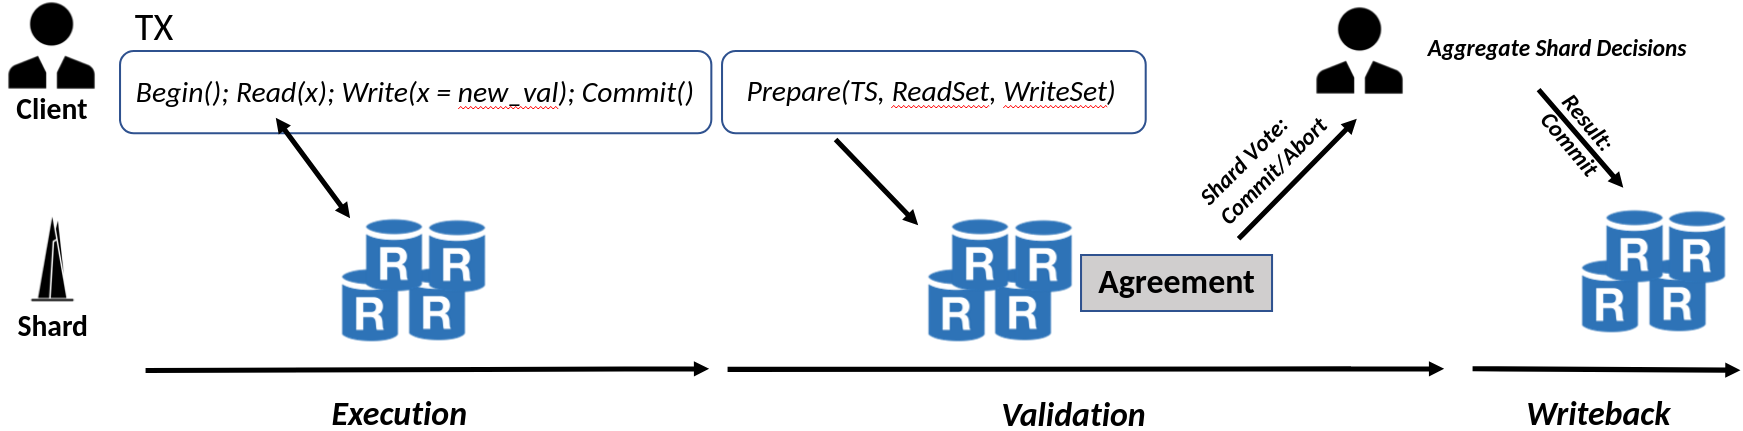
\includegraphics[width= \textwidth]{./figures/LC.png}
\end{center}
\caption{Transaction Lifecycle}
\label{fig:Figure1}
\end{figure*}




%\section{Protocol-Notes}

Structure:\\
0. Preamble what Indicus is and what it is supposed to offer.\\
1. Model., Properties   \\
2. Architecture: Exec, Val, WB, \\

Replica state?\\

3. Exec details: Read/Write Set computation\\
4. Concurrency Control check. Put in relation to Exec details\\
5. Validation Protocol: a) Voting and Decision rule component b) Logging. Explain similarity to other BFT protocols (logging could use anything, in 5f+1 it resembles Q/U because etc.)\\
6. Writeback and Multi-shard TX\\
7. Failures between 5/6\\
8. Optimizations: \\
9. Indicus3: Extra abort phase, different quorums (Validation and View change), Extra proofs\\
10. Correctness proofs: Only for 5f+1?\\
	- ACID: serializable specifically\\
	- Prove recovery maintains same result and consistency\\
	- Prove liveness (i.e. client has all tools necessary: dependency resolution, general aborts/abstains. Fallback live leader election. )\\

\subsection{TX execution}
Goal:\\
- clients should be able to read valid and consistent data from the database\\
- clients should see the most recent data\\


Challenge\\
- Replicas can be out of sync and byzantine\\
- There might be concurrent transactions ongoing that are conflicting\\

Our Design:\\
- Clients speculatively execute their TX: Writes buffered locally, Reads go remote\\
- Reads can read committed and potentially committing values\\
- Necessary quorums sized so validity (and liveness) is maintained

Subtlelties:
- unique TX ID -- avoids equivocation and makes Tx uniquely indexable in efficient data structures
- include dependencies in their TX (f+1 signed copies - Q: Why is this necessary? A: To make replicas believe it exists so that other clients are able to recover that knowledge.)
- 

\subsection{Concurrency control}
Goal: \\(Exceptions, read leases, dependencies: Q: how to store full txid)
- limit aborts\\

challenges:\\
- concurrent read/writes. Maintain isolation: serializability\\
- geo-distributed so execution and validation takes long --> more interleavings\\
- clocks are not perfectly synced\\
- minimize unecessary aborts\\
- byzantine clients can create artificial congestion\\

- Maintain Isolation while replicas out of order. In total order protocols (SMR), deviation from the "common" vote signals misbehavior, whereas for us that is not the case. \\

Our Design:\\
- TSO based concurrency control: Assign optimistic timestamps that define serialization order\\
- Enforce loose bound on the timestamps. This is fine for safety, but necessary to restrict progress damage. Alternative way is to have a TS gen phase, but this induces a RTT and certificate to attach so it is undesirable. Instead we ignore Transactions that are too far in the future, as such reads could make a lot of writes abort. Reads are not affected by writes with large timestamps, since we allow to read from RTS time.\\
- Reads and Writes are tested on Conflicts with previously committed or possibly committing Transactions. Evaluation happens based on TS and whether serialization order would be violated.\\
- MVTSO: 3 techniques to reduce the number of aborts:\\
	- Read from TS, and not newest. This allows reads (especially long reads, which can happen in a WAN network) to avoid aborting due to later writes. This requires a multi version store.\\
	- Read possibly committing writes. This is to avoid missing writes that should have been seen. Effectively minimizes the "lockout window" that the latency of validation-writeback phases incur.\\
	- Reads issue RTS in order to acquire "locks" on concurrent writes that would cause reads to abort. This requires the Timestamp to be known in advance. \\
	
Subtlelties:\\
- concurrent read and dependency validation could make own dependencies abort. This can especially be strategically abused by byz clients. To avoid this, add dependency exceptions: Async read exceptions sent by honest clients to minimize this window.\\
- Read leases: Read "locks" could be arbitrarily acquired by byz clients without intention of completing a TX. Thus they are on a timeout. Larger writes are not affected anyways. Application option: decide who to grant read locks, since they are not a safety mechanism, but an additional progress "shield"\\
- Efficient dependency storage: Only claim dependencies on f+1 for several reasons: a) at least one honest believes this could commit, b) allows to only store TXIDS in a TX and not full dependency, because that dep can be recovered when necessary - having info about deps is necessary for client liveness.\\

- how to bound dep depth? Reads return a field that says dep depth. Honest clients will not create deeper deps. Byzantine Clients may try, but cannot, because the f+1 signed dep messages include the full dep tree, and replicas will not accept any TX that have depth > some d. In practice we probably want d = 1, so the fallback starts directly for the immediate depdency.\\
	- in general it was possible to "miss" comittable/prepared tXs, thats okay since reading prepared is just an optimization.\\
	
- Abort decisions need to come with proofs that client can validate: Avoids fake aborts. In 5f+1 the proof is implicit since f+1 abort votes are necessary.\\
- Optimization: Retries for Writes. Comes at a tradeoff for validation phase latency, so we elaborate only later.\\
-
	
Replica datastructures:
- for efficient lookups we have following data structures:
-   Hashmap from TXIDs to protocol state (for easy management of ongoing TX). 
- Key value store for prepared TX, includes Writes, Reads, and RTS
- Committed State: Key value store of the DB. Allows to Read. Allows to lookup for conflicts.
- Commit Log: Set of TXIDS that are committed (maps TXID to TX)  (allows to check if deps have alreaday committed. 
- Abort Log: See Commit Log (allows to check if dependencies have already aborted)
- Dependency set: Map from TXID to waiting dependents (allows to unblock waiting dependencies when a TX finishes)
- (optional: dependant to dependency mapping. Once mapping is empty, this TX is not waiting on anybody anymore)



\subsection{Validation}
Goal:\\
- maintain ACID guarantees: Isolation, Durability, Atomicity\\
- Be client driven, i.e. leaderless and out of order\\
- avoid frontrunning\\
- be scalable\\
- be fast\\


Challenges:\\
- Maintain Isolation while creating highest chance to commit\\
- Tolerate byzantine replicas voting dishonestly\\
- Tolerate Client failures: equivocation, crashes, stalling, replay\\
--> Answer: make final decisions idempotent\\
- enable consistent recovery\\
- minimize state at replicas while still guaranteeing correct agreement. Make sure local knowledge is enough to guarantee global correctness\\
- minimize necessary roundtrips and communication complexity\\


Basic design:\\
- Voting phase:\\
	- Client sends to all, All to CC check, all reply\\
	- Client makes decision based off Quorum and Decision Rule (have figure for it?)\\
	- Metaphor: Instead of a leader serializing and deciding on a decision, the decisin was made jointly by all replicas. Hence, "voting" phase
	- After the voting phase a TX is persistant (? \fs{technically only needs to be at f+1} and some order is finalized (this order can still change with retries), but the TX is ordered AT least at this spot \fs{super weird phrasing rn, maybe useless for intuition anyways}
	
- Decision rule:\\
	- Since votes can be inconsistent (no total order enforced on replicas) we must aggregate them\\
	- Must be designed in a way that maintains Isolation\\
	- 3f+1 commit necessary. Vice versa, 3f+1 abstain necessary. Absense of enough commit votes requires pessimistic decision in abort.\\
	- Wait up to time out for at least 2f+1. If timeout expires and less than 2f+1, keep waiting. \\
	
- Ordering decision is made without a leader (democratically): Fairness is up to the network\\
	
- Persistant Logging. 2pc analogy. (or is 3pc analogy better?)\\
	- Want to make sure, that whatever client decision was made (equivalent to choice of Vote quorum), is going to be persistent and idempotent. I.e. if commit/abort is returned to the application any re-issue of the protocol (which can be necessary under faults) is consistent with the original decision.\\
	- In 2pc decision is logged to persistant storage. That obviously doesnt work in this setting (byz client, even under crash you would like to make progress). So a Client "logs" the decision by replicating it consistently to the replicas.\\
	- Client sends decision, gets back echo\\
	- If enough consistent echos then the result may return. This guarantees that decision can be recovered.\\
	- 4f+1 matching replies required: We will show recovery later.\\
	
- Any "normal" agreement protocol could be used once a "decision" has been cast, at this point it is just for replication. I.e. one could plug in a leader based consensus mechanism here, but its overkill and unecessary. There are no conflicts anymore, so an order isnt necessary either. Just unordered broadcast/receive is enough: This is exactly Q/U basically. "Contention" is a byzantine client equivocating. Q/U makes the observation that with multiple clients it would not be live, thus we introduce the fallback view change mechanism. \\

Subtlelties:\\
- 5f+1 commit fast path: 3f+1 abstain/abort fast path. (Cannot have these with retries). If Abort includes proof, then 1 abort fast path as well.\\
- 


\subsection{Writeback}
Goal: \\
- Finalize commit/aborts\\
- Maintain consistency\\
- Enable garbage collection\\

Challenges:\\
- client failures (crash, equivocation)\\
- 

Basic Design:\\
- Client uses the Logging certificates to proceed. Aggregates these certificates for every shard.\\
- Any Client can fulfill this role, arbitrary amount in parallel or even Replicas because this operation is guaranteed to be idempotent (due to the validation and recovery logic)\\
- Upon Receiving Commit Abort, Replicas update their data structures. Remove from Prepared strucutres, Add to Commit/Abort Logs. \
- Dont need a dedicated append only ledger (?). It would be different for each replica anyways. Can just store these logs as Hashmaps (i.e. reuse our lookup structures)\\
- 

Subtlelties:\\
- Optimization: Single shard logging\\
- The logging phase is redundant if there are multiple voting shards involved. Instead, the votes could be aggregated BEFORE logging to form the decison and then only be logged on a dedicated shard. This saves communication bandwidth and makes recovery simpler, because there is a dedicated single shard where to look.\\

\subsection{Optimizations}
Goals:\\
- reduce write aborts\\
- reduce redundancy in validation\\
- reduce read lock impact (byz clients)\\

Challenges:\\
- defend against byz client abuse\\
- respect all shard results\\
- 

- Pretty much mentioned in other sections already. Seems like its more suitable to have it with the contet right away.?

\subsection{Granting Liveness}
Goals:\\
- be robust to byzantine client\\


challenges:\\
- byzantine clients can stall or equivocate during Validation/Writeback\\
- replicas can diverge due to byzantine clients. Need to reconcile safely\\
- Granting honest clients liveness --> ability to "realiably" finish all Transactions.\\


Design: \\
- Since the system overall has no shared notion of progress, we maintain liveness only on a per client bases. Specifically, view changing is not only unecessary if nobody cares about a TX but also useless, as no "liveness" is maintained.\\
- View change seperately for every single TX, because every single TX is consensus on a binary register\\
- Since liveness is directly coupled to Clients, view changes should naturally be coupled to clients interest. However, if multiple Clients are able to run the protocol at the same time, then there might never be a conclusion. Electing a single client to be in charge would be very difficult and also not bound the view changes necessary for progress, because there is an unbounded fraction of byz clients\\
- Solution: Delegate view change to a dedicated fixed size group.. The replicas! Gives the guarantee, that when the network is synchronous, after at most f view changes it will succeed. Sync needs to be assumed and thats ok according to FLP.\\
- A little more subtle: After at most f view changes IF an honest client is involved, otherwise no guarantee\\

LIVE ELECTION\\
- Protocol (in theory): Clients issue View change requests for a TX they are interested in. Replicas ONLY move to the next view if a client proves to them, that a Quorum existed in the past view. This guarantees, that replicas cannot diverge arbitrily far in their views. More concretely, there is always >=f+1 honest replicas that dont diverge in views by more than 1 and there are < f+1 honest replicas that diverge from other replicas by more than 1.\\


- Protocol (in practice): To avoid byzantine Clients view changing arbitrarily long and driving up timeouts before honest Clients are interested we introduce some all to all forwarding.
Add additional (off critical viewchange path) exchange to the Fallback replica to issue and disseminate certificates. (Technically equivalent to a Writeback if single sharded. If multi-sharded 2 considerations: a) if not optimized single shard logging, then still need to aggregate decisions, b) if single shard logging, then replica needs to be aware of all other shards in order to forward (can still Writeback locally).\\

SAFE RECOVERY:\\
- Protocol: Choose 2f+1 if existing, otherwise f+1, otherwise redo p2 based on p1. (p1 guaranteed to exist since they voted. Replicas only vote if they had the p1. Client gave it to them if they didnt have it before.) (If replica sees 4f+1 matching right away, it can return that to the client and also distribute as certs)\\
- Clients can only use Quorums from matching views to return to the application (simple counterexample: 3 commits 3 aborts and then swap)\\
- FB can use decisions from multiple views for the decision rule (i.e. decision rule is view agnostic). When could this arise? Because newer views subsume older views and FBs might have been byzantine, or been replaced too quickly. \\
- Proof by Induction: If something returned then ... guaranteed to only ever issue that decision\\
- 



Necessary Extras:\\
- A Client first asks all replicas for existing p2 state or potential certificates. An honest client doesnt need the view change in that case - it was in order to get such certificates.\\
- Client acquires current view from all replicas by doing so. Uses this to start a view change. If f+1 matching exist, client uses those to catch up replicas that lag behind proactively. (just speeds things up: dont need to send all 4f+1)\\
- A client simultaneously re-issues a p1 message, in case some replicas have never seen the TX\\
- A client is repsonsible for the Writeback (any client can do this): Any "interested" client receives the p2 decisions made from a fallback and attempts to return. \\


Subtletlties:\\
- (Maybe useless:) Only a client that provides a dep proof (f+1) or abstain proof is allowed to issue fallback. Doesnt make it impossible to start FB, but at least some hurdle (a client could always just receive such a abstain message with the proof from a byz colluder replica\\
- Fallback election is not started if that TX itself has a dependency - wait for all deps to be finished themselves. This is to distinguish whether a Client has been slow, or its blocking itself due to another dependency.\\
- Tx map to different initial fallbacks: I.e. (TXID + view) mod n \\

\subsection{Byzantine Client behaviors}

- Can acquire random read "locks". Problem: Takes external effect without ever committing anything. Solution: Only grant Read timestamps (locks) to timely clients. 

- Can increase congestion by submitting multiple TX concurrently. Solution: Replicas can vote to abstain on concurrent TX. Disincentivized because Replicas processing 2 TX from 1 client before they have received a commit message can be used as Proof of Misbehavior. (Assume messges from a same client are always fifo, simple to maintain with a sequence number: Dont allow clients to skip sequence numbers. Requires a client to finish up his own TXs if he crashed)

- Can fake read sets: Read illegal values OR not include performed reads. Solution: This is ok according to the Byz-I definition. Such reads only have limited external effect: No more than in simple read/write conflict OCC

- Can fake dependencies: Either equivocate or not include them. Solution: Cannot equivocate without it manifesting as 2 different TX. Not including them is fine, then there is no dependency on which replicas block.

- Arbitrary timestamps. Solution: Bound too large TS because they could create a lot of aborts. Small timestamps are fine, they become obsolete. Can disallow them for garbage collection

- can strategically/reactively make concurrent TXs abort, i.e. "artificial congestion". Solution: Only works reliably if network is under adversarial control.

- Submit two different TX with same TS (TS is not part of ID, due to retries. If retries are disallowed, then this phenomena is impossible). Solution: Break ties via ID. Serves as proof of misbehavior and could be voted to abstain.

- go fast path but retry anyways. Solution: Must disallow one of the options

- can equivocate during agreement. Solution: Quorums make sure only one solution can be returned and that this solution can be maintained. Transforms problem into stalling. In traditional SMR protocols this would eventually trigger a view change once replicas time out.

- can stall during agreement. Solution: Fallback mechanism for interested Client liveness


\subsection{Garbage Collection}
Challenge:
- memory footprint grows large due to multi version
- certificates impose large signature overheads

Options:
- Need to bound and remove versions below watermarks
- In 5f+1 can read based on f+1 matching committed. Dont need certs and can still be safe for recovery and robust to replicas "claiming random dependency aborts"


\subsection{Discussion: }
- Explain/Define Client relative liveness. We dont provide liveness if something is async, "liveness" ill defined for this sort of system. What it means: Clients that follow P experience liveness, but there is no system notion because there is no shared total ledger.  Progress is client relative\\
- Several seperate binary consensus instances \\


optional Extras to mention:
-Can use Witnesses instead of replicas to lighten replication burden
- only need to contain key/version and not values


\subsection{Indicus3}



View changes:
- bounding rule works differently: slightly weaker guarantee
- Decision rule: In View change hierarchy!! I.e. higher view beats anything. Implication: If conflicting decision to previous view was made, then previous view vote could not have been final.
	1. 1 p3 commit: use it to return
	2. 1 p3 abort: re-issue p2 abort 
	3. 1 p2 commit: re-issue p2 commit
	4. 1 p2 abort: re-issue p2 abort OR re-do p1, either works
	5. Nothing: re-issue p2 using p1 decisions.
	
Want the same practical all to all between replicas + fallback async certificates 
%-------------------------------------------------------------------------------
\section{Indicus}
%-------------------------------------------------------------------------------

%-------------------------------------------------------------------------------
%\section{Protocol}
%-------------------------------------------------------------------------------
\begin{figure*}[!th]
\begin{center}
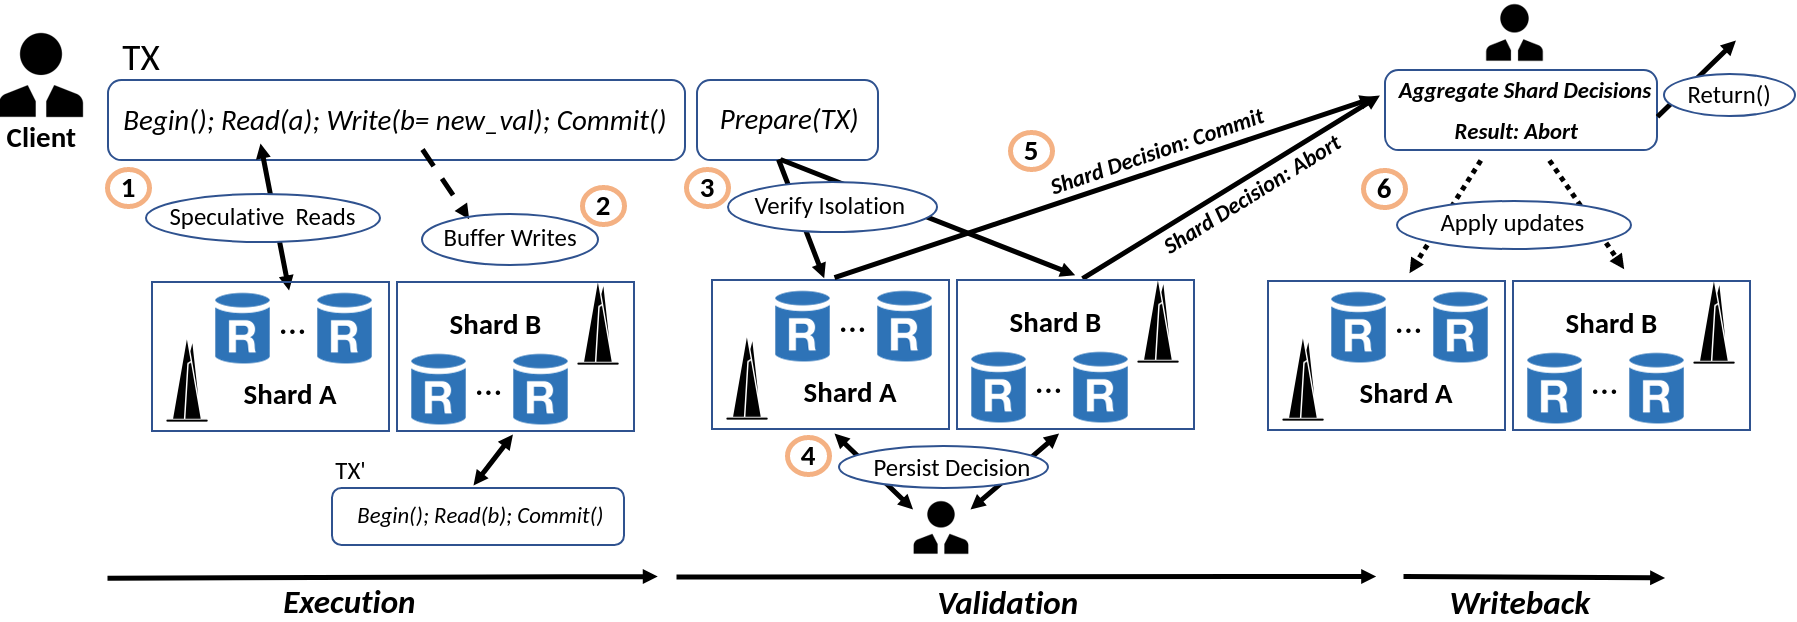
\includegraphics[width= \textwidth]{./figures/Archi.png}
\end{center}
\caption{{\em Transaction Lifecycle}. Clients execute remote reads (1) and buffer writes (2). For Committment, all involved shards verify isolation (3). If there are conflicting transactions (TX'), replicas in a shard (B) vote to Abort. A client persists a decision (4) that serves as Two-Phase-Commit Vote for each shard (5), and Commits a transaction if all shards vote to commit (6).}
\label{fig:Figure1}
\end{figure*}
\fs{cut figure if it is not useful} \nc{I don't figure hurts, but I don't think it helps much either}\la{I would tentatively remove it: we are probably going to need the space}

\sys is is a sharded and replicated transactional key-value store designed to be scalable and leaderless, and our architecture reflects this ethos. \sys{} 

\par \textbf{Transaction Execution} Transaction execution is driven by clients (removing costly all-to-all communications amongst replicas) and consists of three phases. First, in an \textit{execution phase}, clients execute individual transactional operations. As is standard in optimistic databases, reads are submitted to remote replicas while writes are buffered locally. \sys{} supports \textit{interactive} and cross-shard transactions: clients can issue new operations based on the results of past operations to any shard in the system. \sys{} must additionally ensure that these read operations do not violate Byzantine independence. In a second \textit{validation phase}, invidual shards in \sys{} must validate whether committing the transaction would violate serializability. For performance, \sys{} allows invidiual replicas within a shard to process requests out of order. \sys{} must additionally ensure that Byzantine actors cannot cause spurious aborts. Finally, \sys{} aggregates each shard decision in a \textit{commit phase} to determines the outcome of the transaction, notifies both application and replicas in the system of the decision, and, if the decision was to commit, makes the buffered writes persistent int he data store.  Importantly, the decision of whether each transaction commits or aborts must be preserved across failures, reconfigurations, and Byzantine attacks. We describe each of these phases in turn in Section~\ref{}

\par \textbf{Transaction Recovery} A Byzantine actor could begin executing a transaction, start the validation phase, but intentionally never reveal its decision. Without care,
such behavior would prevent the system from making progress, violating Byzantine independence. To ensure progress, \sys{} thus implements a fallback recovery mechanism that can terminate stalled transactions while maintaining serializability. We describe this mechanism in Section~\ref{}.




\nc{Florian's version in comments}
\iffalse
\sys is designed to be scalable and leaderless. Our architecture reflects this ethos. We briefly summarise it here before going into more detail in the later sections. 
In \sys, clients drive the entire transaction life cycle which can be broken down into three stages as shown in Figure \ref{fig:Figure1}: i) Execution, ii) Validation, and iii) Writeback. 
i) Clients \textit{speculatively execute} transactions themselves, invoking only remote read procedure calls (1) and buffering writes locally (2). \two Clients validate initiate a two-phase commit vote to validate speculative execution results for byzantine-serializability (3).
For every involved shard, a client queries potentially inconsistent replicas for their commitment vote, reconciles divergent votes into a single per-shard decision that maintains Isolation, and make this decision durable to avoid replay of contradictory decisions (4). 
iii) Lastly, clients aggregate all shard decisions (5) for atomic commit, return to the application and asynchronously, \textit{writes back} decisions and database updates (6).

Next, we outline the protocols for Execution, Validation and Writeback respectively. 
\fi

\fs{longer version in Architecture.tex }






\iffalse
\fs{since this only affect validation, maybe move it there.}
\sys comes in two different flavors, \sys{}3 and \sys{}5 respectively, that rely on varying replication degrees, but implement the same design. \sys{}3 requires $n=3f+1$ replicas \fs{, the minimum bound necessary for BFT SMR?,} per shard to guarantee consistency in the presence of $\leq f$ byzantine replicas. \sys{}5 reduces both latencies during failure free execution and complexity during recovery. \footnote{We believe that consortiums with high performance requirements or high replication degrees are respectively comfortable with paying for additional replicas or tolerating a lower fraction (1/3 vs 1/5) of failures}
For the simplicity of exposition we discuss \sys{}5 for the remainder of the paper, and defer to section X \fs{and/or TR} to describe differences in \sys{}3. In the following, we outline \sys 's execution (unaffected by replication degree), validation and writeback protocols.

\fi



%\fs{whole section probably needs to fit in max 2 pages}

\sys{}'s execution protocol has three goals: 1) to offer clients an interactive transaction interface \fs{too obvious?}, 2) to be scalable, and 3) to maintain independent operability \fs{and Byzantine independence, Serializability}.

\sys{} achieves these goals by combining optimistic client-side execution with an aggressive, but Byzantine resilient, concurrency control (CC) scheme that maintains Byz-Serializability. 
\iffalse
 \la{We seem to have already made this points in the intro tio the section} \changebars{}{\sys leaves clients responsible for executing the transactions they submit, and allows every client, in parallel, to execute arbitrary interactive transactions using read RPC's, instead of submitting stored procedured that must be ordered and executed by replica servers.}  
 \fi By relying on optimistic rather than pessimistic CC schemes such as 2-phase-locking (2PL), \sys{} forgoes costly coordination to acquire locks, and sidesteps the concern of Byzantine clients refusing to relinquish locks.

\iffalse
\la{I would just remove the following} 
\changebars{}{Before we detail Indicus’s transaction processing and validation mechanism, we first discuss the CC that Indicus imple- ments as the latter are functions of the precise CC requirements.}
\fi

\subsection{\sys{}'s Concurrency Control}

%%% Explain MVTSO itself only briefly. Then explain how we make it for for byz
% 1) bound timestamps, 2) make writes visible late only, 3) only allow f+1 matchin uncommitted writes, 4) read timestamps
%Afterwards: explain execution interface. After that explain validation check. Then have overarching example
\iffalse
% we need to change a few things:
0) timestmap bound
1) Read validity
2) deferred writes
3) read uncommitted
4) byz read timestamps (read lock implies you had access control, at that point it is no different than issuing a tx and completing. But we do not want to give the power to abort for no reason. It should be traceable.
\fi

\fs{fig doesnt make so much sense before reading the whole thing} \fs{cut this preamble?}
Figure \ref{fig:MVTSOEX} shows an example trace of \sys operational behaviors under different request processing orders (assume $f=1$) that we use to guide the remaining outline.

\begin{figure*}
\begin{center}
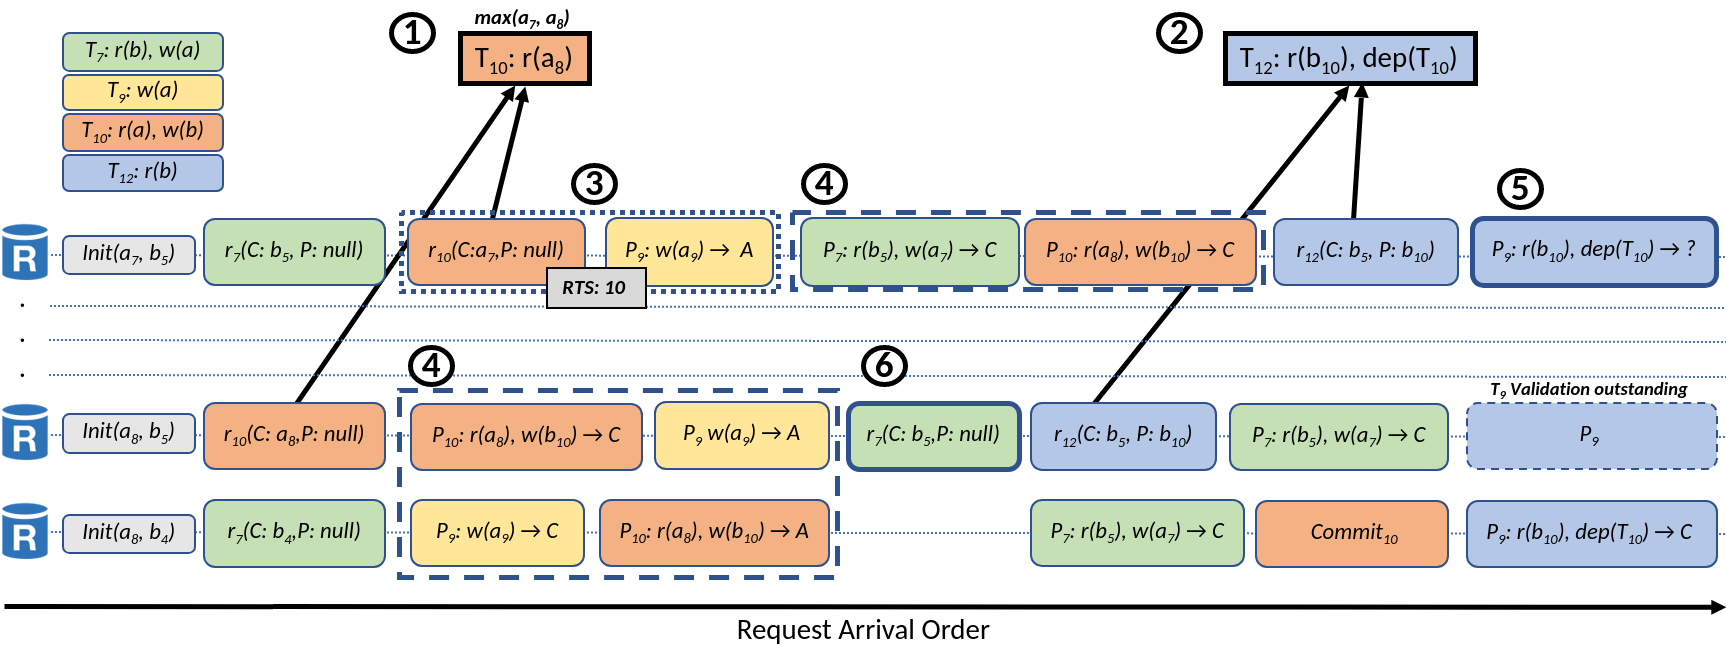
\includegraphics[width= \textwidth]{./figures/MVTSOLargeFont.png}
\end{center}
\caption{\emph{MVTSO behavior for different replica processing orders}. $r_x(C : a_y ,P : a_z)$ denotes that transaction $T_x$ (x being the timestamp of a transaction in this example) reads the version $y$ of object a written by committed transaction $T_y$ and version $z$ from tentative prepared transaction $T_z$. $P_x(RS,WS,DEP)$ denotes a transaction $T_x$'s prepare request (i.e. the validation check) for respective ReadSet (RS), WriteSet (WS) and Dependenc Set (DEP), and $\rightarrow C / A$ denotes the local replica validation outcome (Commit/Abort).} 
\label{fig:MVTSOEX}
\end{figure*}

\par \textbf{MVTSO.} Our starting point is Multiversioned Timestamp Ordering (MVTSO), a concurrency control scheme which prescribes a serialization order by assigning a speculative timestamp \textit{before} execution \cite{bernstein1983multiversion, reed1983implementing, su2017tebaldi}. In MVTSO, read operations return the latest written version smaller than the readers' timestamps. Respectively, writers attempt to create new versions at their timestamp, but must abort if a higher timestamped read would have "missed the write" by reading a prior version. A transaction may commit only, if all read-write dependencies have committed.

\iffalse
\fs{cut the whole following paragraph?} \la{Yes, I would cut it} This allows us to a) only classify concurent read/write operations as conflicting if their execution results violate the timestamp order (Fig. \ref{fig:MVTSOEX}: 4 bottom), and b) avoid write/write conflicts alltogether. 
When speculative execution results match the pre-defined timestamp order, no aborts are necessary (Fig. \ref{fig:MVTSOEX}: 4 top). \sys{}'s challenge is therefore to a) assign appropriate timestamps and b) coordinate execution in a way that maximizes such coherence; the presence of Byzantine participants (clients/replicas) complicates this.

In MVTSO, reads operations return the latest written version smaller than the readers' timestamps, while writers attempt to create new versions at their timestamp, but must abort if a higher timestamped read would have "missed the write" by reading a prior version. A transaction may commit only, if all read-write dependencies have committed.
\fi

When \sys{}'s speculative execution results match the pre-defined timestamp order, no aborts are necessary (Fig. \ref{fig:MVTSOEX}: 4). \sys{}'s challenge is therefore to a) assign appropriate timestamps and b) coordinate execution in a way that maximizes such coherence; the presence of Byzantine participants (clients/replicas) complicates this.

\par \textbf{Byzantine resilience.} Read operations in \sys have the following sub-goals: \one Correct clients should read valid data, i.e. experience read integrity, \two Correct clients should read fresh data, i.e. minimize staleness and hence maximize commit chance, and \three Reads must provide the context necessary to potentially complete observed write state. 
Clients validate the integrity of reads by requiring replicas to provide a proof of validity, which consists of a set of signatures confirming committment, or if not yet existant, a set of  $f+1$ replica's tentative commit endorsements \fs{maybe cut this second part, since it will become redundant}. Moreover, to guarantee that clients do not read maliciously stale data from their local replica, \sys encourages clients to read the latest version across $\geq f+1$ replicas (Fig. \ref{fig:MVTSOEX}: 1,2).
Avoiding Byzantine influence comes at a cost: Read operations require a synchronous, potentially WAN \fs{or just remote - i.e. not local}, rountrip. 

MVTSO intuitively synergizes well with \sys{}'s potenially WAN remote reads as reading from a fixed timestamp helps speculative readers observe consistent snapshots, even when execution is long and consequently interleavings are frequent (Fig. \ref{fig:MVTSOEX}: 6). \fs{at the price of experiencing serializability instead of strict serializability - that is only the case if your timestamps are outdated}.

While we assume that clocks are loosely synchronized across correct participants, Byzantine participants may diverge arbitrarily and propose excessively high timestamps. A simple solution is to bound time-stamps by querying the median time from a Quorum of replicas and including replies as proof \cite{bazzi2004non, bazzi2018clairvoyant}. To side-step the additional overheadd that a dedicated timestamping phase incurs, we compromise by allowing clients to optimistically select their own timestamps, but reject request timestamps above a threshold at all correct replicas, thus incentivising clients to select bounded, close to real-time, timestamps. 

In traditional MVTSO, writes become visible to successive, higher timestamped, reads immediately. However, in the presence of Byzantine clients this is undesirable, as it allows clients to issue write operations without the intention of ever committing a transaction. Thus, any correct clients' read that observes, and consequently depends on a Byzantine clients write may be blocked indefinitely.
%Allowing other clients to preemtively commit outstanding write operations is infeasible, as the remaining transaction procedure is known only to the issuing client, while conceiding pessimistic abort permission empowers Byzantine participants to obstruct any correct clients' writes. 
\sys reconciles this dilemma by deferring all database updates until execution is complete and the client prepares the transaction for commitment. 
% Concretely, \sys clients buffer all write operations, and submit them only when attempting to commit the transaction, thereby enabling other \sys client to orderly complete Validation and Writeback steps.\\
\la{This needs to be better explained} \fs{took a pass:}
Clients in \sys distinguish explicitly between writes \textit{committed} across all involved shards and tentative writes \textit{prepared} at a single shard: While clients accept all verifiable \textit{committed} version from a single replica, they accept \textit{prepared} versions only when endorsed by $f+1$ replicas. This ensures that a) at least one correct replica believes that the write can commit, and hence is worth observing, and b) that Byzantine replicas and clients cannot collude to violate Byzantine independence by reactively inventing versions. \fs{such invented transactions could be designed to be guaranteed to abort: I.e. by claiming to have read an out-dated version. The write versions could be engineered to be perfectly at the bound of the read timestamp, such that it is guaranteed to be chosen}\\
Finally, \sys replicas evaluate writes for conflicts by maintaining a Read Timestamps (RTS) for each locally processed read (Fig. \ref{fig:MVTSOEX}: 3). While this allows un-prepared reads to elicit external effects, these affect only concurrent transactions with smaller timestamps and can be bypassed by re-trying a transaction. To nonetheless limit recurrent abuse, we discuss a personalized lease mechanism to limit Byzantine influence in section Y.z (Optional Modifc). \fs{or just do it here in 1-2 sentences. We do not implement this though.}



\subsection{Execution interface}
Client applications execute transactions via the following interface. A TX object \textit{TXObj $\coloneqq$ (SeqNo, ClientID, InvolvedShards, ReadSet, WriteSet, Dependencies)}, records the state necessary for Validation.

\iffalse
\begin{figure}
\begin{center}
\includegraphics[width= 0.5\textwidth]{./figures/TxState.png}
\end{center}
\caption{Transaction execution state}
\label{fig:Txstate}
\end{figure}
\fi

\textbf{Begin()} A client begins a transaction by optimistically choosing a timestamp \textit{TS $\coloneqq$ (Time, ClientID)} that defines a total serialization order across all clients.  \\
\textbf{Write(key, value)}. A client buffers the write: \textit{WriteSet = WriteSet $\cup$ (key, value)}\\
%%%%%%%%%Read protocol%%%%%%%%%%%
\textbf{Read(key, TS, RQS)} 
If \textit{key $\in$ WriteSet} a client returns the buffered write value. Otherwise, the client conducts a remote read for given hyperparameter Read Quorum Size (RQS):

\fbox{\begin{minipage}{23em}

\textbf{1: C} $\rightarrow$ \textbf{R}: Client sends read request to Replicas
\end{minipage}}\\
%Improve RQS formulation
A client broadcasts a read request  $m = (Read, key, TS)_c$.
\iffalse
 to $RQS$ different replicas. Note, that in order to guarantee $\geq RQS$ replies a client might need to send up to $f$ additional requests to compensate for unresponsive/faulty participants ($max(|Replies|) \leq n-f$). 
\fi
\fs{Optimization: A client sends only to RQS+f to receive RQS many replies}

\fbox{\begin{minipage}{23em}
\textbf{2: R} $\rightarrow$ \textbf{C}: Replica processes client read and replies
\end{minipage}}\\
A replica authenticates the client\footnote{Byzantine replica may ignore read access control. Solving this problem is beyond the scope of this work; we defer to existing solutions \cite{basu2019efficient}.}, and enforces a local timestamp threshold. \fs{this can probably be shortened:} It returns a signed message \text{$\langle \textit{ReadReply, Committed, Prepared} \rangle _R$}, where $Committed \coloneqq (value, version, proof)$ represents the value-version pair with largest committed write version smaller than TS and a proof of commitment,  and $Prepared \coloneqq (value, version, TxID', deps)$ the respective largest uncommitted value-version pair, the associated transaction ID, and the latter transactions potentially uncommitted read-write dependencies. Moreover, a Replica stores a new read timestamp (RTS) for the key: $RTS(key) = RTS(key) \cup TS$ (Fig. \ref{fig:MVTSOEX}: 3). 
\fs{a replica may include a set of prepared values to increase likelihood of client receiving f+1 matching}

\fbox{\begin{minipage}{23em}
\textbf{3: C} ($\rightarrow$ \textbf{R}): Client receives read replies 
\end{minipage}}\\
A client waits for $\geq RQS$ read replies and chooses the biggest valid result \textit{(value, version) $= max_{valid}$(\{Committed\},\{Prepared\}} (Figure \ref{fig:MVTSOEX}: 1,2). A \textit{Committed} tuple is valid, if the proof confirms commitment, wheras a \textit{Prepared} is valid iff there exist $f+1$ matching \textit{Prepared$_r$}. The client adds the version to its read set \textit{ReadSet = ReadSet $\cup$ (key, version)} and additionally claims a dependency if it was a \textit{Prepared} version: \textit{Dep = Dep $\cup$ \{f+1 $\times$ Prepared$_r$ \}} . 

\fs{la: finds the use of commit in both exec and validation confusing. Is it unclear that this refers to application here?}
\textbf{Commit()} A Client terminates its execution, and computes a unique transaction identifier based on final execution object and its timestamp: $TxID \coloneqq (H(TxObj, TS)$, thus preculding Byzantine participants from equivocating transaction contents. It then initiates the Validation Phase by issuing a 2PC-Prepare requests to each involved shard.
%What if a byz doesnt send to all involved shards? It will be visible on some shard and hence an correct client can obtain the full TX. See Hierarchical IDS in Protocol.tex

\textbf{Abort()} A client terminates execution, and broadcasts a request to release all acquired Read Timestamps (RTS). Since writes in \sys are deferred, no other rollback action is necessary.


We briefly discuss some implications of the choice of Read Quorum Size (RQS). Following cases may be distinguished: \one \textbf{$RQS = 1$} A client may read committed data from just \textit{trusted} replica (at the risk of reading stale data) to reduce execution latency and consequently minimize conflicting interleavings. \two \textbf{$RQS \geq f+1$} \sys{}'s recommended minimal mode of operation. While side-stepping maliciously stale reads, it is still possible to read (arbitrarily) stale data due to replica inconsistency, caused by either asynchrony or partial transaction replication by a Byzantine client.
\three \textbf{$RQS \geq \frac{n+f+1}{2}$} When reading from a Quorum of sufficient size to overlap with any Validation Quorum (ref section Validation) in at least one correct replica, a client guarantees, that no more \textbf{additional} (beyond previously observed) conflicting writes can be admitted, since such a Quorum of acquired RTS acts as a read-lock. 

\iffalse
Trusting only $f+1$ matching prepared writes has the beneficiary side effect of allowing us to include only transaction identifiers as dependencies, rather than the full transaction, since it is guaranteed that at least one correct replica has stored the transaction. Thus, in the failure free scenario, where clients need not complete transactions $in Dep$, \sys minimizes the meta-data overhead that the recovery protocol imposes.
\fi

We remark that, consistent with Byz-Isolation, \sys allows Byzantine clients to fabricate and (permissibly) submit arbitrary reads; Byzantine clients may \textit{choose} whether to read legal, or even real data.  \sys does, however, enforce that Byzantine clients cannot (undetectably) fabricate dependencies by requiring a proof of $f+1$ matching prepared writes. This precludes Byzantine clients from indetectibly stalling their own transactions and consequently obstructing liveness for consecutive descendant (second degree...) dependencies.
Furthermore, this allows \sys to include only transaction identifiers as dependencies, rather than the full transaction, thereby minimizing the common path overhead. The full transaction can be acquired from an correct replica when necessary. We discuss how to complete stalled or slow transactions in section Y (Granting Liveness).





%
\subsection{Validation Check}

Algorithm \ref{mvtso} shows the necessary validation check to preserve Byzantine-Serializability. 
Given a transactions prepare request the validation check returns an Abort vote if a conflict has been detected, and Commit otherwise. 
When execution results match the timestamp order, there are no conflicts (Fig. \ref{fig:MVTSOEX}: 4 top). For each read, a replica verifies that it has not voted to commit a conflicting write (Algorithm \ref{mvtso}, line 3-7). Conversely, for each write, a replica confirms that there exist no previously accepted reads (line 8-10), and no ongoing read transactions (line 11-12) that conflict. Fig. \ref{fig:MVTSOEX}: 4 shows both non-conflicting and conflicting interleavings.
If there are no conflicts, a replica tentatively \textit{prepares} a transaction, making its writes visible and evaluating future transactions against it for conflicts. Regardless of the outcome, a replica garbage collects all Read Timestmaps (RTS) associated with the transactions reads.
It then waits for necessary dependencies (uncommited writes that were read) to be resolved (Figure \ref{fig:MVTSOEX}: 5). We remark, that the concurrency control check is serialized and executed atomically for each transaction.

\begin{theorem}
The set of transactions for which the MVTSO-Check returns Commit is Byzantine-Serializable. 
\end{theorem}
\begin{proof}
See TR.
\end{proof}

\begin{algorithm}
\caption{MVTSO-Check(TX, TS)}\label{mvtso}
\begin{algorithmic}[1]
\If{\textit{$TS > localClock + \delta$}} %  || $TS < lowWM$ || $\exists d \in dep: d.TS < lowWM$} } dont mention garbage collection part here, it only confuses
\State \Return Abort
\EndIf

\For{\textit{$\forall key,version \in \textit{TX.RS}$}}
        \If{$ \exists TX2 \in Committed \cup Prepared: key \in \textit{TX2.WS} $ \newline
        \hspace*{2em} $\land \, version < \textit{TX2.TS} < TS$}  
          \State  \Return Abort, \textit{TX2, (TX2.CommitProof)}  
         \EndIf  
\EndFor

\For{\textit{$\forall key \in \textit{TX.WS}$}}
        \If{$\exists TX2 \in Committed \cup Prepared:$ \newline 
        \hspace*{2em} $\textit{TX2.RS[key].version} < TS < TX2.TS$} 
          \State  \Return Abort, \textit{TX2, (TX2.CommitProof)}
         
        \EndIf
        \If{$\exists RTS \in key.RTS: RTS > TS$} 
          \State  \Return Abort
       \EndIf
\EndFor
\State Prepared.add(TX) 

\While{$\exists d \in dep: d \notin CommitLog \cup AbortLog $)}
\State Suspend
\EndWhile

%structure it in a way that is better
\For{\textit{$\forall d \in dep$}}
		\If{$ d \in AbortLog $}
		\State	Prepare.remove(TX)
		\State \Return Abort, \textit{(TX2.AbortProof)}
		\EndIf
\EndFor
\State \Return Commit
\end{algorithmic}

\end{algorithm}

In order to perform the MVTSO-check, a replica maintains several data strucutres: \one It stores read timestamps, read versions alongside the multiversioned write stores for committed and tenative transactions respectively, to provide efficient evaluation of conflicts.
\two In order to confirm dependency outcomes, replicas log proofs for completed transactions in respective Commit and Abort Log sets, that together induce the ledger of all processed transactions. 
\three To avoid busy waiting when dependencies are not yet resolved, a replica temporarily suspends the MVTSO-check for the current transaction, allowing it to process other transactions pending validation. To facilitate this, it keeps track of an additonal transaction to dependents mapping that allows to identify and resume all suspended MVTSO-checks associated with dependents of a completing transaction.

\iffalse

\textit{Aside:} Consistent with our definition of Byzantine-Isolation, byzantine clients may issue ficticious Read-Sets comprised of arbitrary read versions and values. However, these have only limited external effect on concurrent writes. We distinguish two extreme cases: 1) $read.version \rightarrow 0$: This case is equivalent to simply reading stale data, and effectively reduces MVTSO to TSO as conlflicts are evaluated only on basis of the transaction timestamps (i.e. Abort write if: write.TS < read.TS). 2) $read.version \rightarrow read.TS$: In this case there are no conflicts as a write is never "missed" by a previous read.
\fi

In the following section we will show how to design a replicated validation scheme that upholds Isolation guarantees and reaches a single shard decision, even when replicas within a shard validate in different orders.


%%-------------------------------------------------------------------------------
\subsection{Validation Phase}
%-------------------------------------------------------------------------------

In order to facilitate atomic committment across all shards involved in a transaction \sys clients invoke a Prepare request, inquiring each shard to validate the transaction for conflicts and cast a 2PC vote. Shards in \sys are replicated for fault tolerance.

\fs{idk where to put this and whether to mention at all - but we do want to state that there exists a version with 3f+1 (minimal replication degree) that implements the same ethos }
\sys comes in two different flavors, \sys{}3 and \sys{}5 respectively, that rely on varying replication degrees, but implement the same design. \sys{}3 requires $n=3f+1$ replicas \fs{, the minimum bound necessary for BFT SMR?,} per shard to guarantee consistency in the presence of $\leq f$ byzantine replicas. \sys{}5 reduces both latencies during failure free execution and complexity during recovery. \footnote{We believe that consortiums with high performance requirements or high replication degrees are respectively comfortable with paying for additional replicas or tolerating a lower fraction (1/3 vs 1/5) of failures}
For the simplicity of exposition we discuss \sys{}5 for the remainder of the paper, and defer to section X \fs{and/or TR} to describe differences in \sys{}3. In the following, we outline \sys 's execution (unaffected by replication degree), validation and writeback protocols.

The goals of the Validation phase are threefold: \one It must decide on a single, durable vote per-shard that maintains Byzantine Serializability (henceforth we refer to this as a \textit{shard-decision}), \two It should be leaderless, and not enforce unecessary ordering for commutative, non-conflicting transactions, and \three It must preserve independent operability. \fs{needs to refer to the fallback}

Satisfying these goals requires ovecoming several challenges. In order to maximize parallelism and embrace partial ordering, \sys allows replicas to process requests out of order. Consequently, replicas may temporarily diverge, and hence return different validation results. Such divergence must be reconciled in a way that maintains Isolation, but not overly conservatively in order to bound the impact of byzantine participants and maximize likehlihood to commit. \sys designates clients as validation coordinator for its own transactions, thus omitting a dedicated replica leader. %The respective protocol must tolerate client failures such as crashes, omission/stalling, equivocation, or replays and allow for consistent recovery. 

The Validation protocol can be broken down into two functionalities: Voting and Logging.
Since \sys replicas may process requests in different order, they must reach consensus on a joint  decision. To do so, they cast a vote for their local validation result, which are subsequently democratically aggregated into a decision. In the case of Indicus, the client acts as the transaction coordinator who aggregates and relays results (along with necessary evidence).
In order to maintain consistency in the presence of failures (no two honest replicas finalize different Commit/Abort decisions), this decision must be durable and unique, guaranteeing that a replay of any Writeback is idempotent. However, since a byzantine coordinator cannot be trusted to durably store a decision, nor could we retain liveness during a crash or partition, \sys demands clients to \textit{log} the decision at replicas before returning.
 

The voting step requires a single round-trip to all replicas, whereas the logging phase requires at most one round-trip \fs{in Indicus5 and at most two round-trips in Indicus3.}. When execution is fault- and contention free transactions can be committed on the \textit{Fast-Path} in a single-round trip as an explicit logging round is not necessary.


%%%%%%%%%% protocol
To describe how the protocol operates in detail we follow a single-shard transaction through the system:

\fbox{\begin{minipage}{23em}
\textbf{(1: C $\rightarrow$ R)}: Client sends Prepare request to all Replicas within the Shard.
\end{minipage}}\\
Upon deciding to Commit in the Execution phase, a Client initiates Validation by sending a message $Phase1 \coloneqq \langle Prepare, TxID, TX \rangle_{\sigma_c}$ to all Replicas.

\fbox{\begin{minipage}{23em}
\textbf{(2: R $\rightarrow$ C)}: Replica receives validation request, processes it and returns vote to Client.
\end{minipage}}\\
A replica validates Timestamp and Dependency integrity of the request. It then evaluates Read and Write Sets for Isolation conflicts against its local state using the MVTSO Concurrency Control Check (CCC), as shown in algorithm 1. It returns a message $Phase1R \coloneqq \langle TxID, vote \rangle_r$, and optionally evidence in case it voted to Abort.

\underline{Additional subtlelties}: 
A replica never changes its Voting decision, because re-execution could leave to different results. Once the MVTSO-Ceck completes (i.e. there are no blocking dependencies), a replica starts a timer to monitor the clients progress.

\fbox{\begin{minipage}{23em}
\textbf{(3: C)}: Client waits for vote replies.
\end{minipage}}\\
A client waits for at least $n-f$ ($4f+1$ in Indicus5) distinct replica votes, or more, up to a system specified timeout. 

\fbox{\begin{minipage}{23em}
\textbf{(3a: C)}: Client receives Threshold of matching votes and returns to application. Proceeds to Writeback
\end{minipage}}\\
In any of the following 3 cases, a client may short-circuit waiting for additional votes and omit a dedicated Logging round:
\begin{enumerate}
\item \textbf{$1$ Abort vote w/ Conflicting TX \& CommitCertificate}: A conflict with a commited transaction. The client validates the integrity of the CommitCertificate and returns the shard decision $(TxID, Abort, \langle ConflTX \rangle_{CC})$. 
\item \textbf{$3f+1$ Abort votes w/ Conflicting TX}: A conflict with a prepared, but not yet committed transaction. The client returns the shard decision $(TxID, Abort, \{\langle AbstainVote\rangle_r\})$. 
\item \textbf{$5f+1$ Commit votes}: No conflicts. The client returns the shard decision $(TxID, Commit, \{\langle CommitVote \rangle_r\}$
\end{enumerate}
Any of such Quorums forms a \textit{Shard-Certificate} and proves the decision. A client uses this Certificate to return to its application and issue the Writeback.

\fbox{\begin{minipage}{23em}
\textbf{(3b: C $\rightarrow$ R)}: Client receives divergent results and suggests a consistent decision to Replicas for Logging
\end{minipage}}\\
If a client does not receive the necessary thresholds of votes to return, it must continue on the \textit{Slow-Path}. To do so, it aggregates the votes according to following decison rule:
If there exists a $CommitQuorum \coloneqq \frac{n+f+1}{2}$ of Commit Votes, the Slow-Path decision is Commit, otherwise it is Abort.
A client broadcasts a message $Phase2 \coloneqq (TxID, decision)_c, \{\langle votes \rangle_r\}$.

\underline{Additional subtlelties}: A client forwards a Quorum of $\geq n-f$ votes to the replicas in order to prove the Slow-Path decision is consistent with Isolation guarantees. Note, that a byzantine client may equivocate the decision by relaying different Quorums.

\fbox{\begin{minipage}{23em}
\textbf{(4: R $\rightarrow$ C)}: Replicas receive, validate and echo decision
\end{minipage}}\\
A replica confirms that the Decision matches the Quorum by evaluating the decision rule itself and adopting the decision. It then returns the decision to the client by sending $Phase2R \coloneqq \langle TxID, decision \rangle_r$. Importantly, a replica never changes its decision.

\fbox{\begin{minipage}{23em}
\textbf{(5: C)}: Client returns shard-decision to application and proceeds to Writeback
\end{minipage}}\\
A client waits for a Quorum of $n-f$ matching $Phase2R$ messages. Such a Quorum forms a \textit{Shard-Certificate} and proves the decision. A client uses this Certificate to return to its application and issue the Writeback.

\underline{Additional subtlelties}: If a client equivocated, it will never receive a Shard-Certificate. An honest client however, is guaranteed to receive matching Phase2 replies. 

We consider a decision (Commit, Abort) to be \textit{logged} when it is possible for some Shard-Certificate to exist, i.e. as soon as the necessary certificate Quorums exists at some Replicas.
Figure \ref{fig:FigureSP} summarizes the relevant nomenclature.

\begin{figure}
\begin{center}
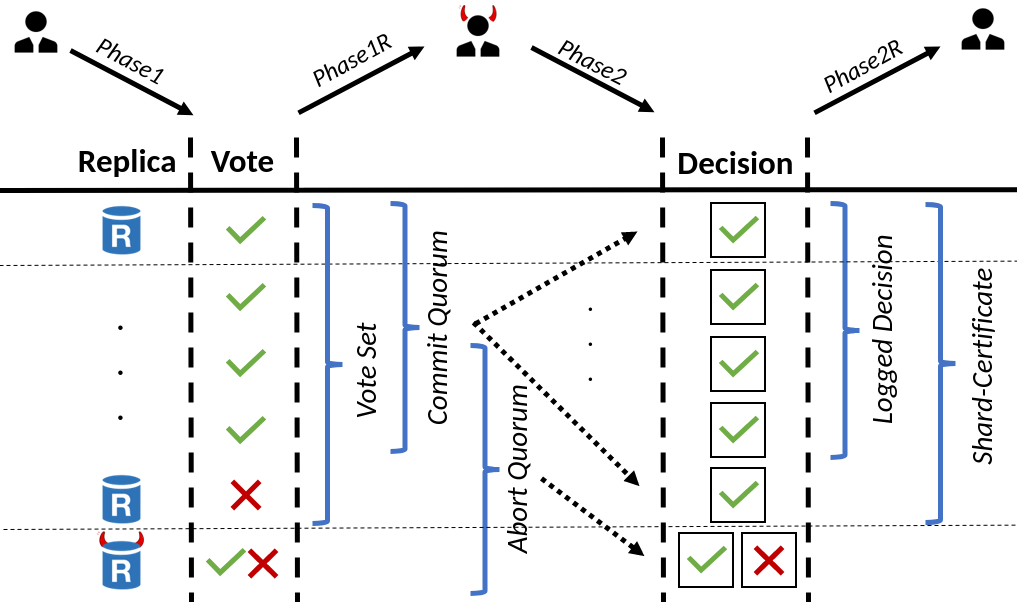
\includegraphics[width= 0.5\textwidth]{./figures/Nom2.png}
\end{center}
\caption{Validation Nomenclature, Slow-Path. Note, that a byzantine client may equivocate Phase2 decisions by including Commit and Abort Quorums respectively. Byantine replicas may store multiple votes and decisions.}
\label{fig:FigureSP}
\end{figure}

\subsubsection{Correctness}
We show, that a \textit{logged} decision is final:
\begin{theorem}[Saf]
A logged decision is durable, and there can ever exist \textbf{at most one} logged decision.
\end{theorem}
\begin{proof}
See TR.
\end{proof} 

Note, that since replicas never change their decision, it is possible for there to never be any logged decision if a byzantine client equivocated its Slow-Path Quorums. In order to reconcile this, we design and discuss a recovery mechanism in section X which relaxes the requirement on persisting a decision.  


\begin{theorem} 
Indicus maintains \textit{Byzantine-Serializability}.
\end{theorem}
To prove that this is the case, we show that for any two conflicting transactions, at most one can be committed.
\begin{proof}
See TR.
\end{proof}

\begin{theorem} 
Indicus maintains Byzantine Independence in the absence of network adversary.
\end{theorem}

We show, that once a Client submits a transaction for validation, the result cannot be unilaterally decided by any byzantine participant, be it client or replica.
\begin{proof}
See TR.
\end{proof}

%%-------------------------------------------------------------------------------
\subsection{Writeback}
%-------------------------------------------------------------------------------



%\subsection{Multi-sharding}

and Multi-shard 2pc

- Optimization: Single shard logging


%%-------------------------------------------------------------------------------
\subsection{Failures}
%-------------------------------------------------------------------------------
- Fallback: election (only starts if not waiting on another dep to avoid early eviction), views, resolution, subtelties with mvtso (block because of dep), necessity even without dependencies. Interested clients, write-back multishard. garbage collection
- Fallback requires an extra round in order to learn about current views to start viewchange, but thats ok: Its co-function with learning about full TX, and checking for existing certificates. Timeout invocation is concurrent with p1 message.



%%-------------------------------------------------------------------------------
\section{Further optimizations}
%-------------------------------------------------------------------------------


\fs{the current writeback might be unecessary to explain, since we implement the below anyways... Perhaps merge writeback and this subsection}
\par \textbf{Shard Logging} When transaction execution touches multiple shards validation can incur redundant explicit logging overhead. When a Slow-Path is necessary to arrive at a logged decision on S different shards, bandwith is wasted. Consider an example in which $S-1$ shards attempt to log the decision Commit, while a single shard attempts to log an Abort decision. If the latter shard succeeds, the effort of the remaining shards was in vain. \fs{Moreover, logging is always bottlenecked by the slowest shard. }
The culprit of this phenomenon is the delayal of Two-Phase-Commit (2PC) until the Writeback phase. By preemptively making a 2PC decision \textbf{before} logging we can avoid this redundancy. We remark, that even when when all shards agree on a decision, this saves redundant coordination. \fs{This does not work for Atomic Broadcast! In AB, the voting only happens AFTER the tx has already been logged (i.e. the order has been durably replicated)}

Concretely, we designate \textbf{one} involved shard as \textit{logging Shard} $=$ \textit{involvedShards[TxID \% |involvedShard|]}, while all other shards remain responsible only for Voting. \changebars{}{The logging Shard can be determin via a determinsitic function over the \textit{involved Shards}. A simple load balanced solution may select $loggingS = involvedShards[TxID \% |involvedShard|]$}. \changebars{}{Figure \ref{fig:SingleShardOpt} shows a comparison and the revised structure. dont use this figure in actual paper} In order to log a decision, Phase1R Quorums \fs{aka shard votes} from all involved shards are required. We modify step 3 of the Validation protocol accordingly:

\fbox{\begin{minipage}{21em}
\textbf{Validation (3: C)}: Client waits for vote replies from all involved Shards.
\end{minipage}}
A client aggregates a per-shard decision for each shard according to the \textit{CommitQuorum} rule. If all shard-decisions are Commit, it attempts to log a Commit decision by sending $Phase2 \coloneqq (TxID, Commit, S \times \{CommitQuorum\}$ to all replicas in the designated logging Shard. If a single shard-decision is Abort, it stops waiting for other shard-decisions and attempts to log an Abort decision by instead sending $Phase2 \coloneqq (TxID, Abort, AbortQuorum)$. 

\underline{Additional subtlelties:} A client can go Fast-Path and return to the Writeback phase immediately only if Fast-Path Quorums were received for all shards. 

The remaining Validation protocol proceeds identically to the multi-shard version. Notice, that when only a single shard is involved, no adjustments were made. The Writeback phase instead, may proceed with just the single certificate from the logging Shard


The Fallback protocol is adjusted accordingly: A fallback replica need (and can) only be elected on the logging Shard, simplifying reconciliation and reducing the cost for interested clients. 
To further reduce unecessary load, a client may attempt to first inquire whether decisions exists at the logging shard (Fallback protocol step 1 \& 2), before sending $Rec-Phase1$ messages to all shards in order to gather votes itself (Fallback protocol step 1). 

\iffalse
\begin{figure*}
\begin{center}
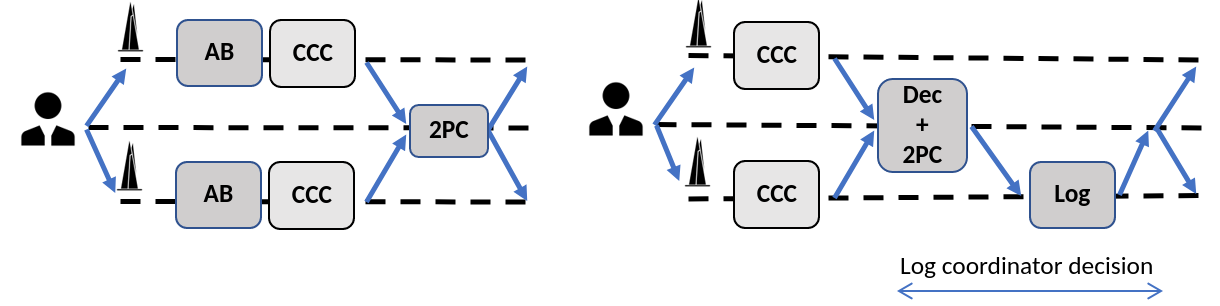
\includegraphics[width= \textwidth]{./figures/SingleShard.png}
\end{center}
\caption{Single Shard Optimization}
\label{fig:SingleShardOpt}
\end{figure*}
\fi

\par \textbf{Batching}
To amortize cryptographic overheads we introduce message batching. However, unlike leader based systems, in \sys there exists no central sequencer that may batch request. Instead, \sys implements message batching at the replicas by batching $b$ messages, generating a merkle tree \cite{merkle1987digital}, and signing only the root hash, thus reducing signing overheads from $O(b)$ to $O(1)$ per batch. The merkle hash tree allows replicas to respond to individual clients by including only the single client-addressed message and $log(b)$ additional hashes. We note, that since replicas receive requests out of order, their batches are not consistent. Consequently, a client must aggregate hashes and signatures from different merkle trees to forward as proofs (Phase2 and Writeback messages include $O(n)$ signatures and hashes) .
In order to reduce verification overheads from $O(n*b)$ to $O(n)$, replicas cache previously verified signatures by storing a mapping from signature to merkle hash roots. For following message verifications, a replica can omit de-computing the signature, and must only re-compute and compare the merkle root based on the hashes included in the proof.

\iffalse
- amortize signature cost
- unlike leader based, there is not an obvious sequencer to batch
- instead we batch signature generation at replica. Because they can be out of order these batches are different. Also do not want to send the whole batch (b* hashes) to every client. Instead we use a merkle tree and send only the root sig + log(b) hashes. (this means that we had to do 2*b hashes during signature gen, but we only do b*log(b) hashes at generation instead of b*b. OR: could send whole batch of  messages --> huge message + hashing cost..
- Cache already validated signatures at replicas and only recompute the hash to see whether it matches. This reduces verification by a factor of b (effectively only verifying for the first message from the batch).
\fi

\par Other non impelmented opts: in TR.

 

\fs{whole section probably needs to fit in max 2 pages}

\sys{}'s execution protocol has three goals: 1) to offer clients an interactive transaction interface \fs{too obvious?}, 2) to be scalable, and 3) to maintain independent operability \fs{and Byzantine independence, Serializability}.

\sys{} achieves these goals by combining optimistic client-side execution with an aggressive, but Byzantine resilient, concurrency control (CC) scheme that maintains Byz-Serializability. 
\iffalse
 \la{We seem to have already made this points in the intro tio the section} \changebars{}{\sys leaves clients responsible for executing the transactions they submit, and allows every client, in parallel, to execute arbitrary interactive transactions using read RPC's, instead of submitting stored procedured that must be ordered and executed by replica servers.}  
 \fi By relying on optimistic rather than pessimistic CC schemes such as 2-phase-locking (2PL), \sys{} forgoes costly coordination to acquire locks, and sidesteps the concern of Byzantine clients refusing to relinquish locks.

\iffalse
\la{I would just remove the following} 
\changebars{}{Before we detail Indicus’s transaction processing and validation mechanism, we first discuss the CC that Indicus imple- ments as the latter are functions of the precise CC requirements.}
\fi

\subsection{\sys{}'s Concurrency Control}

%%% Explain MVTSO itself only briefly. Then explain how we make it for for byz
% 1) bound timestamps, 2) make writes visible late only, 3) only allow f+1 matchin uncommitted writes, 4) read timestamps
%Afterwards: explain execution interface. After that explain validation check. Then have overarching example
\iffalse
% we need to change a few things:
0) timestmap bound
1) Read validity
2) deferred writes
3) read uncommitted
4) byz read timestamps (read lock implies you had access control, at that point it is no different than issuing a tx and completing. But we do not want to give the power to abort for no reason. It should be traceable.
\fi

\fs{fig doesnt make so much sense before reading the whole thing} \fs{cut this preamble?}
Figure \ref{fig:MVTSOEX} shows an example trace of \sys operational behaviors under different request processing orders (assume $f=1$) that we use to guide the remaining outline.

\begin{figure*}
\begin{center}
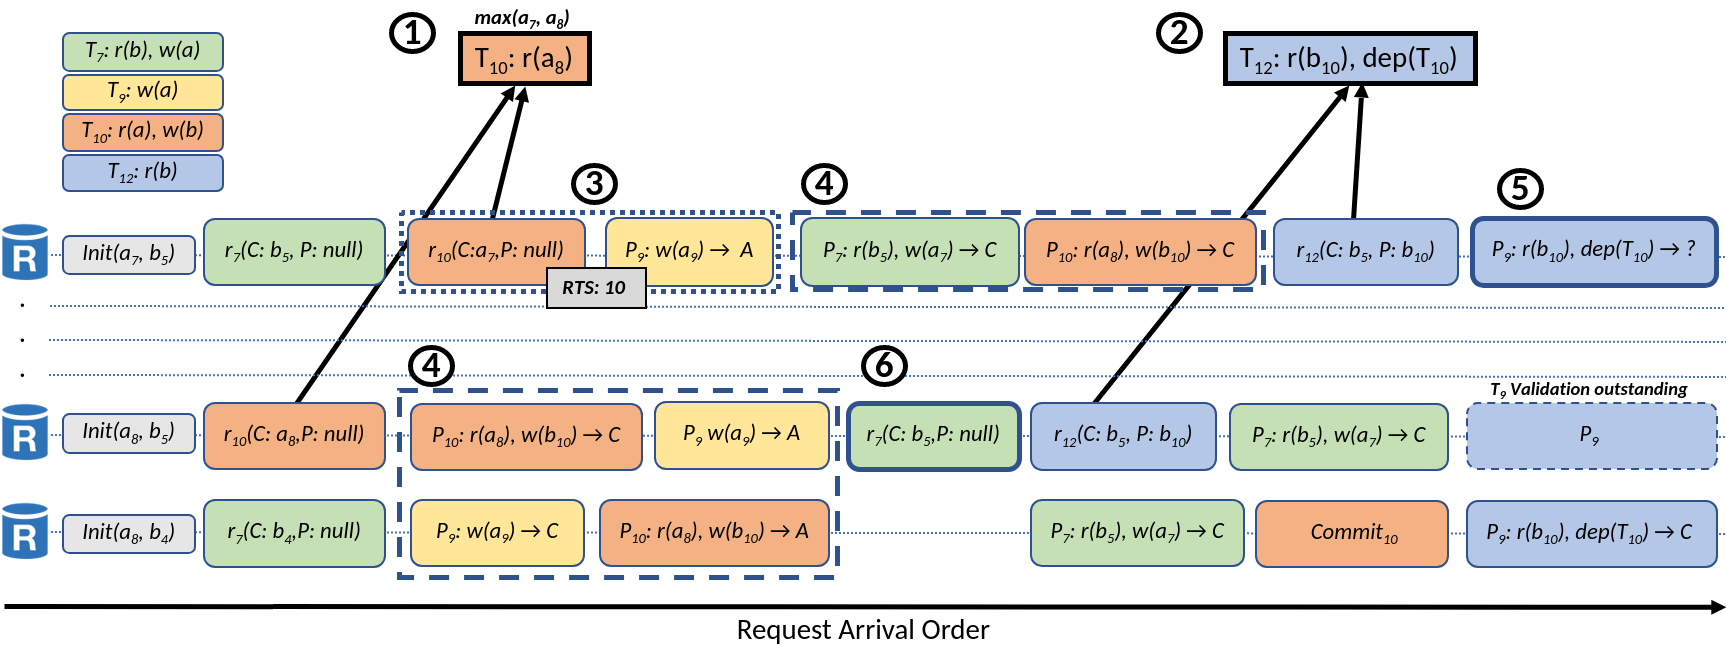
\includegraphics[width= \textwidth]{./figures/MVTSOLargeFont.png}
\end{center}
\caption{\emph{MVTSO behavior for different replica processing orders}. $r_x(C : a_y ,P : a_z)$ denotes that transaction $T_x$ (x being the timestamp of a transaction in this example) reads the version $y$ of object a written by committed transaction $T_y$ and version $z$ from tentative prepared transaction $T_z$. $P_x(RS,WS,DEP)$ denotes a transaction $T_x$'s prepare request (i.e. the validation check) for respective ReadSet (RS), WriteSet (WS) and Dependenc Set (DEP), and $\rightarrow C / A$ denotes the local replica validation outcome (Commit/Abort).} 
\label{fig:MVTSOEX}
\end{figure*}

\par \textbf{MVTSO.} Our starting point is Multiversioned Timestamp Ordering (MVTSO), a concurrency control scheme which prescribes a serialization order by assigning a speculative timestamp \textit{before} execution \cite{bernstein1983multiversion, reed1983implementing, su2017tebaldi}. In MVTSO, read operations return the latest written version smaller than the readers' timestamps. Respectively, writers attempt to create new versions at their timestamp, but must abort if a higher timestamped read would have "missed the write" by reading a prior version. A transaction may commit only, if all read-write dependencies have committed.

\iffalse
\fs{cut the whole following paragraph?} \la{Yes, I would cut it} This allows us to a) only classify concurent read/write operations as conflicting if their execution results violate the timestamp order (Fig. \ref{fig:MVTSOEX}: 4 bottom), and b) avoid write/write conflicts alltogether. 
When speculative execution results match the pre-defined timestamp order, no aborts are necessary (Fig. \ref{fig:MVTSOEX}: 4 top). \sys{}'s challenge is therefore to a) assign appropriate timestamps and b) coordinate execution in a way that maximizes such coherence; the presence of Byzantine participants (clients/replicas) complicates this.

In MVTSO, reads operations return the latest written version smaller than the readers' timestamps, while writers attempt to create new versions at their timestamp, but must abort if a higher timestamped read would have "missed the write" by reading a prior version. A transaction may commit only, if all read-write dependencies have committed.
\fi

When \sys{}'s speculative execution results match the pre-defined timestamp order, no aborts are necessary (Fig. \ref{fig:MVTSOEX}: 4). \sys{}'s challenge is therefore to a) assign appropriate timestamps and b) coordinate execution in a way that maximizes such coherence; the presence of Byzantine participants (clients/replicas) complicates this.

\par \textbf{Byzantine resilience.} Read operations in \sys have the following sub-goals: \one Correct clients should read valid data, i.e. experience read integrity, \two Correct clients should read fresh data, i.e. minimize staleness and hence maximize commit chance, and \three Reads must provide the context necessary to potentially complete observed write state. 
Clients validate the integrity of reads by requiring replicas to provide a proof of validity, which consists of a set of signatures confirming committment, or if not yet existant, a set of  $f+1$ replica's tentative commit endorsements \fs{maybe cut this second part, since it will become redundant}. Moreover, to guarantee that clients do not read maliciously stale data from their local replica, \sys encourages clients to read the latest version across $\geq f+1$ replicas (Fig. \ref{fig:MVTSOEX}: 1,2).
Avoiding Byzantine influence comes at a cost: Read operations require a synchronous, potentially WAN \fs{or just remote - i.e. not local}, rountrip. 

MVTSO intuitively synergizes well with \sys{}'s potenially WAN remote reads as reading from a fixed timestamp helps speculative readers observe consistent snapshots, even when execution is long and consequently interleavings are frequent (Fig. \ref{fig:MVTSOEX}: 6). \fs{at the price of experiencing serializability instead of strict serializability - that is only the case if your timestamps are outdated}.

While we assume that clocks are loosely synchronized across correct participants, Byzantine participants may diverge arbitrarily and propose excessively high timestamps. A simple solution is to bound time-stamps by querying the median time from a Quorum of replicas and including replies as proof \cite{bazzi2004non, bazzi2018clairvoyant}. To side-step the additional overheadd that a dedicated timestamping phase incurs, we compromise by allowing clients to optimistically select their own timestamps, but reject request timestamps above a threshold at all correct replicas, thus incentivising clients to select bounded, close to real-time, timestamps. 

In traditional MVTSO, writes become visible to successive, higher timestamped, reads immediately. However, in the presence of Byzantine clients this is undesirable, as it allows clients to issue write operations without the intention of ever committing a transaction. Thus, any correct clients' read that observes, and consequently depends on a Byzantine clients write may be blocked indefinitely.
%Allowing other clients to preemtively commit outstanding write operations is infeasible, as the remaining transaction procedure is known only to the issuing client, while conceiding pessimistic abort permission empowers Byzantine participants to obstruct any correct clients' writes. 
\sys reconciles this dilemma by deferring all database updates until execution is complete and the client prepares the transaction for commitment. 
% Concretely, \sys clients buffer all write operations, and submit them only when attempting to commit the transaction, thereby enabling other \sys client to orderly complete Validation and Writeback steps.\\
\la{This needs to be better explained} \fs{took a pass:}
Clients in \sys distinguish explicitly between writes \textit{committed} across all involved shards and tentative writes \textit{prepared} at a single shard: While clients accept all verifiable \textit{committed} version from a single replica, they accept \textit{prepared} versions only when endorsed by $f+1$ replicas. This ensures that a) at least one correct replica believes that the write can commit, and hence is worth observing, and b) that Byzantine replicas and clients cannot collude to violate Byzantine independence by reactively inventing versions. \fs{such invented transactions could be designed to be guaranteed to abort: I.e. by claiming to have read an out-dated version. The write versions could be engineered to be perfectly at the bound of the read timestamp, such that it is guaranteed to be chosen}\\
Finally, \sys replicas evaluate writes for conflicts by maintaining a Read Timestamps (RTS) for each locally processed read (Fig. \ref{fig:MVTSOEX}: 3). While this allows un-prepared reads to elicit external effects, these affect only concurrent transactions with smaller timestamps and can be bypassed by re-trying a transaction. To nonetheless limit recurrent abuse, we discuss a personalized lease mechanism to limit Byzantine influence in section Y.z (Optional Modifc). \fs{or just do it here in 1-2 sentences. We do not implement this though.}



\subsection{Execution interface}
Client applications execute transactions via the following interface. A TX object \textit{TXObj $\coloneqq$ (SeqNo, ClientID, InvolvedShards, ReadSet, WriteSet, Dependencies)}, records the state necessary for Validation.

\iffalse
\begin{figure}
\begin{center}
\includegraphics[width= 0.5\textwidth]{./figures/TxState.png}
\end{center}
\caption{Transaction execution state}
\label{fig:Txstate}
\end{figure}
\fi

\textbf{Begin()} A client begins a transaction by optimistically choosing a timestamp \textit{TS $\coloneqq$ (Time, ClientID)} that defines a total serialization order across all clients.  \\
\textbf{Write(key, value)}. A client buffers the write: \textit{WriteSet = WriteSet $\cup$ (key, value)}\\
%%%%%%%%%Read protocol%%%%%%%%%%%
\textbf{Read(key, TS, RQS)} 
If \textit{key $\in$ WriteSet} a client returns the buffered write value. Otherwise, the client conducts a remote read for given hyperparameter Read Quorum Size (RQS):

\fbox{\begin{minipage}{23em}

\textbf{1: C} $\rightarrow$ \textbf{R}: Client sends read request to Replicas
\end{minipage}}\\
%Improve RQS formulation
A client broadcasts a read request  $m = (Read, key, TS)_c$.
\iffalse
 to $RQS$ different replicas. Note, that in order to guarantee $\geq RQS$ replies a client might need to send up to $f$ additional requests to compensate for unresponsive/faulty participants ($max(|Replies|) \leq n-f$). 
\fi
\fs{Optimization: A client sends only to RQS+f to receive RQS many replies}

\fbox{\begin{minipage}{23em}
\textbf{2: R} $\rightarrow$ \textbf{C}: Replica processes client read and replies
\end{minipage}}\\
A replica authenticates the client\footnote{Byzantine replica may ignore read access control. Solving this problem is beyond the scope of this work; we defer to existing solutions \cite{basu2019efficient}.}, and enforces a local timestamp threshold. \fs{this can probably be shortened:} It returns a signed message \text{$\langle \textit{ReadReply, Committed, Prepared} \rangle _R$}, where $Committed \coloneqq (value, version, proof)$ represents the value-version pair with largest committed write version smaller than TS and a proof of commitment,  and $Prepared \coloneqq (value, version, TxID', deps)$ the respective largest uncommitted value-version pair, the associated transaction ID, and the latter transactions potentially uncommitted read-write dependencies. Moreover, a Replica stores a new read timestamp (RTS) for the key: $RTS(key) = RTS(key) \cup TS$ (Fig. \ref{fig:MVTSOEX}: 3). 
\fs{a replica may include a set of prepared values to increase likelihood of client receiving f+1 matching}

\fbox{\begin{minipage}{23em}
\textbf{3: C} ($\rightarrow$ \textbf{R}): Client receives read replies 
\end{minipage}}\\
A client waits for $\geq RQS$ read replies and chooses the biggest valid result \textit{(value, version) $= max_{valid}$(\{Committed\},\{Prepared\}} (Figure \ref{fig:MVTSOEX}: 1,2). A \textit{Committed} tuple is valid, if the proof confirms commitment, wheras a \textit{Prepared} is valid iff there exist $f+1$ matching \textit{Prepared$_r$}. The client adds the version to its read set \textit{ReadSet = ReadSet $\cup$ (key, version)} and additionally claims a dependency if it was a \textit{Prepared} version: \textit{Dep = Dep $\cup$ \{f+1 $\times$ Prepared$_r$ \}} . 

\fs{la: finds the use of commit in both exec and validation confusing. Is it unclear that this refers to application here?}
\textbf{Commit()} A Client terminates its execution, and computes a unique transaction identifier based on final execution object and its timestamp: $TxID \coloneqq (H(TxObj, TS)$, thus preculding Byzantine participants from equivocating transaction contents. It then initiates the Validation Phase by issuing a 2PC-Prepare requests to each involved shard.
%What if a byz doesnt send to all involved shards? It will be visible on some shard and hence an correct client can obtain the full TX. See Hierarchical IDS in Protocol.tex

\textbf{Abort()} A client terminates execution, and broadcasts a request to release all acquired Read Timestamps (RTS). Since writes in \sys are deferred, no other rollback action is necessary.


We briefly discuss some implications of the choice of Read Quorum Size (RQS). Following cases may be distinguished: \one \textbf{$RQS = 1$} A client may read committed data from just \textit{trusted} replica (at the risk of reading stale data) to reduce execution latency and consequently minimize conflicting interleavings. \two \textbf{$RQS \geq f+1$} \sys{}'s recommended minimal mode of operation. While side-stepping maliciously stale reads, it is still possible to read (arbitrarily) stale data due to replica inconsistency, caused by either asynchrony or partial transaction replication by a Byzantine client.
\three \textbf{$RQS \geq \frac{n+f+1}{2}$} When reading from a Quorum of sufficient size to overlap with any Validation Quorum (ref section Validation) in at least one correct replica, a client guarantees, that no more \textbf{additional} (beyond previously observed) conflicting writes can be admitted, since such a Quorum of acquired RTS acts as a read-lock. 

\iffalse
Trusting only $f+1$ matching prepared writes has the beneficiary side effect of allowing us to include only transaction identifiers as dependencies, rather than the full transaction, since it is guaranteed that at least one correct replica has stored the transaction. Thus, in the failure free scenario, where clients need not complete transactions $in Dep$, \sys minimizes the meta-data overhead that the recovery protocol imposes.
\fi

We remark that, consistent with Byz-Isolation, \sys allows Byzantine clients to fabricate and (permissibly) submit arbitrary reads; Byzantine clients may \textit{choose} whether to read legal, or even real data.  \sys does, however, enforce that Byzantine clients cannot (undetectably) fabricate dependencies by requiring a proof of $f+1$ matching prepared writes. This precludes Byzantine clients from indetectibly stalling their own transactions and consequently obstructing liveness for consecutive descendant (second degree...) dependencies.
Furthermore, this allows \sys to include only transaction identifiers as dependencies, rather than the full transaction, thereby minimizing the common path overhead. The full transaction can be acquired from an correct replica when necessary. We discuss how to complete stalled or slow transactions in section Y (Granting Liveness).






\subsection{Validation Check}

Algorithm \ref{mvtso} shows the necessary validation check to preserve Byzantine-Serializability. 
Given a transactions prepare request the validation check returns an Abort vote if a conflict has been detected, and Commit otherwise. 
When execution results match the timestamp order, there are no conflicts (Fig. \ref{fig:MVTSOEX}: 4 top). For each read, a replica verifies that it has not voted to commit a conflicting write (Algorithm \ref{mvtso}, line 3-7). Conversely, for each write, a replica confirms that there exist no previously accepted reads (line 8-10), and no ongoing read transactions (line 11-12) that conflict. Fig. \ref{fig:MVTSOEX}: 4 shows both non-conflicting and conflicting interleavings.
If there are no conflicts, a replica tentatively \textit{prepares} a transaction, making its writes visible and evaluating future transactions against it for conflicts. Regardless of the outcome, a replica garbage collects all Read Timestmaps (RTS) associated with the transactions reads.
It then waits for necessary dependencies (uncommited writes that were read) to be resolved (Figure \ref{fig:MVTSOEX}: 5). We remark, that the concurrency control check is serialized and executed atomically for each transaction.

\begin{theorem}
The set of transactions for which the MVTSO-Check returns Commit is Byzantine-Serializable. 
\end{theorem}
\begin{proof}
See TR.
\end{proof}

\begin{algorithm}
\caption{MVTSO-Check(TX, TS)}\label{mvtso}
\begin{algorithmic}[1]
\If{\textit{$TS > localClock + \delta$}} %  || $TS < lowWM$ || $\exists d \in dep: d.TS < lowWM$} } dont mention garbage collection part here, it only confuses
\State \Return Abort
\EndIf

\For{\textit{$\forall key,version \in \textit{TX.RS}$}}
        \If{$ \exists TX2 \in Committed \cup Prepared: key \in \textit{TX2.WS} $ \newline
        \hspace*{2em} $\land \, version < \textit{TX2.TS} < TS$}  
          \State  \Return Abort, \textit{TX2, (TX2.CommitProof)}  
         \EndIf  
\EndFor

\For{\textit{$\forall key \in \textit{TX.WS}$}}
        \If{$\exists TX2 \in Committed \cup Prepared:$ \newline 
        \hspace*{2em} $\textit{TX2.RS[key].version} < TS < TX2.TS$} 
          \State  \Return Abort, \textit{TX2, (TX2.CommitProof)}
         
        \EndIf
        \If{$\exists RTS \in key.RTS: RTS > TS$} 
          \State  \Return Abort
       \EndIf
\EndFor
\State Prepared.add(TX) 

\While{$\exists d \in dep: d \notin CommitLog \cup AbortLog $)}
\State Suspend
\EndWhile

%structure it in a way that is better
\For{\textit{$\forall d \in dep$}}
		\If{$ d \in AbortLog $}
		\State	Prepare.remove(TX)
		\State \Return Abort, \textit{(TX2.AbortProof)}
		\EndIf
\EndFor
\State \Return Commit
\end{algorithmic}

\end{algorithm}

In order to perform the MVTSO-check, a replica maintains several data strucutres: \one It stores read timestamps, read versions alongside the multiversioned write stores for committed and tenative transactions respectively, to provide efficient evaluation of conflicts.
\two In order to confirm dependency outcomes, replicas log proofs for completed transactions in respective Commit and Abort Log sets, that together induce the ledger of all processed transactions. 
\three To avoid busy waiting when dependencies are not yet resolved, a replica temporarily suspends the MVTSO-check for the current transaction, allowing it to process other transactions pending validation. To facilitate this, it keeps track of an additonal transaction to dependents mapping that allows to identify and resume all suspended MVTSO-checks associated with dependents of a completing transaction.

\iffalse

\textit{Aside:} Consistent with our definition of Byzantine-Isolation, byzantine clients may issue ficticious Read-Sets comprised of arbitrary read versions and values. However, these have only limited external effect on concurrent writes. We distinguish two extreme cases: 1) $read.version \rightarrow 0$: This case is equivalent to simply reading stale data, and effectively reduces MVTSO to TSO as conlflicts are evaluated only on basis of the transaction timestamps (i.e. Abort write if: write.TS < read.TS). 2) $read.version \rightarrow read.TS$: In this case there are no conflicts as a write is never "missed" by a previous read.
\fi

In the following section we will show how to design a replicated validation scheme that upholds Isolation guarantees and reaches a single shard decision, even when replicas within a shard validate in different orders.

%-------------------------------------------------------------------------------
\subsection{Validation Phase}
%-------------------------------------------------------------------------------

In order to facilitate atomic committment across all shards involved in a transaction \sys clients invoke a Prepare request, inquiring each shard to validate the transaction for conflicts and cast a 2PC vote. Shards in \sys are replicated for fault tolerance.

\fs{idk where to put this and whether to mention at all - but we do want to state that there exists a version with 3f+1 (minimal replication degree) that implements the same ethos }
\sys comes in two different flavors, \sys{}3 and \sys{}5 respectively, that rely on varying replication degrees, but implement the same design. \sys{}3 requires $n=3f+1$ replicas \fs{, the minimum bound necessary for BFT SMR?,} per shard to guarantee consistency in the presence of $\leq f$ byzantine replicas. \sys{}5 reduces both latencies during failure free execution and complexity during recovery. \footnote{We believe that consortiums with high performance requirements or high replication degrees are respectively comfortable with paying for additional replicas or tolerating a lower fraction (1/3 vs 1/5) of failures}
For the simplicity of exposition we discuss \sys{}5 for the remainder of the paper, and defer to section X \fs{and/or TR} to describe differences in \sys{}3. In the following, we outline \sys 's execution (unaffected by replication degree), validation and writeback protocols.

The goals of the Validation phase are threefold: \one It must decide on a single, durable vote per-shard that maintains Byzantine Serializability (henceforth we refer to this as a \textit{shard-decision}), \two It should be leaderless, and not enforce unecessary ordering for commutative, non-conflicting transactions, and \three It must preserve independent operability. \fs{needs to refer to the fallback}

Satisfying these goals requires ovecoming several challenges. In order to maximize parallelism and embrace partial ordering, \sys allows replicas to process requests out of order. Consequently, replicas may temporarily diverge, and hence return different validation results. Such divergence must be reconciled in a way that maintains Isolation, but not overly conservatively in order to bound the impact of byzantine participants and maximize likehlihood to commit. \sys designates clients as validation coordinator for its own transactions, thus omitting a dedicated replica leader. %The respective protocol must tolerate client failures such as crashes, omission/stalling, equivocation, or replays and allow for consistent recovery. 

The Validation protocol can be broken down into two functionalities: Voting and Logging.
Since \sys replicas may process requests in different order, they must reach consensus on a joint  decision. To do so, they cast a vote for their local validation result, which are subsequently democratically aggregated into a decision. In the case of Indicus, the client acts as the transaction coordinator who aggregates and relays results (along with necessary evidence).
In order to maintain consistency in the presence of failures (no two honest replicas finalize different Commit/Abort decisions), this decision must be durable and unique, guaranteeing that a replay of any Writeback is idempotent. However, since a byzantine coordinator cannot be trusted to durably store a decision, nor could we retain liveness during a crash or partition, \sys demands clients to \textit{log} the decision at replicas before returning.
 

The voting step requires a single round-trip to all replicas, whereas the logging phase requires at most one round-trip \fs{in Indicus5 and at most two round-trips in Indicus3.}. When execution is fault- and contention free transactions can be committed on the \textit{Fast-Path} in a single-round trip as an explicit logging round is not necessary.


%%%%%%%%%% protocol
To describe how the protocol operates in detail we follow a single-shard transaction through the system:

\fbox{\begin{minipage}{23em}
\textbf{(1: C $\rightarrow$ R)}: Client sends Prepare request to all Replicas within the Shard.
\end{minipage}}\\
Upon deciding to Commit in the Execution phase, a Client initiates Validation by sending a message $Phase1 \coloneqq \langle Prepare, TxID, TX \rangle_{\sigma_c}$ to all Replicas.

\fbox{\begin{minipage}{23em}
\textbf{(2: R $\rightarrow$ C)}: Replica receives validation request, processes it and returns vote to Client.
\end{minipage}}\\
A replica validates Timestamp and Dependency integrity of the request. It then evaluates Read and Write Sets for Isolation conflicts against its local state using the MVTSO Concurrency Control Check (CCC), as shown in algorithm 1. It returns a message $Phase1R \coloneqq \langle TxID, vote \rangle_r$, and optionally evidence in case it voted to Abort.

\underline{Additional subtlelties}: 
A replica never changes its Voting decision, because re-execution could leave to different results. Once the MVTSO-Ceck completes (i.e. there are no blocking dependencies), a replica starts a timer to monitor the clients progress.

\fbox{\begin{minipage}{23em}
\textbf{(3: C)}: Client waits for vote replies.
\end{minipage}}\\
A client waits for at least $n-f$ ($4f+1$ in Indicus5) distinct replica votes, or more, up to a system specified timeout. 

\fbox{\begin{minipage}{23em}
\textbf{(3a: C)}: Client receives Threshold of matching votes and returns to application. Proceeds to Writeback
\end{minipage}}\\
In any of the following 3 cases, a client may short-circuit waiting for additional votes and omit a dedicated Logging round:
\begin{enumerate}
\item \textbf{$1$ Abort vote w/ Conflicting TX \& CommitCertificate}: A conflict with a commited transaction. The client validates the integrity of the CommitCertificate and returns the shard decision $(TxID, Abort, \langle ConflTX \rangle_{CC})$. 
\item \textbf{$3f+1$ Abort votes w/ Conflicting TX}: A conflict with a prepared, but not yet committed transaction. The client returns the shard decision $(TxID, Abort, \{\langle AbstainVote\rangle_r\})$. 
\item \textbf{$5f+1$ Commit votes}: No conflicts. The client returns the shard decision $(TxID, Commit, \{\langle CommitVote \rangle_r\}$
\end{enumerate}
Any of such Quorums forms a \textit{Shard-Certificate} and proves the decision. A client uses this Certificate to return to its application and issue the Writeback.

\fbox{\begin{minipage}{23em}
\textbf{(3b: C $\rightarrow$ R)}: Client receives divergent results and suggests a consistent decision to Replicas for Logging
\end{minipage}}\\
If a client does not receive the necessary thresholds of votes to return, it must continue on the \textit{Slow-Path}. To do so, it aggregates the votes according to following decison rule:
If there exists a $CommitQuorum \coloneqq \frac{n+f+1}{2}$ of Commit Votes, the Slow-Path decision is Commit, otherwise it is Abort.
A client broadcasts a message $Phase2 \coloneqq (TxID, decision)_c, \{\langle votes \rangle_r\}$.

\underline{Additional subtlelties}: A client forwards a Quorum of $\geq n-f$ votes to the replicas in order to prove the Slow-Path decision is consistent with Isolation guarantees. Note, that a byzantine client may equivocate the decision by relaying different Quorums.

\fbox{\begin{minipage}{23em}
\textbf{(4: R $\rightarrow$ C)}: Replicas receive, validate and echo decision
\end{minipage}}\\
A replica confirms that the Decision matches the Quorum by evaluating the decision rule itself and adopting the decision. It then returns the decision to the client by sending $Phase2R \coloneqq \langle TxID, decision \rangle_r$. Importantly, a replica never changes its decision.

\fbox{\begin{minipage}{23em}
\textbf{(5: C)}: Client returns shard-decision to application and proceeds to Writeback
\end{minipage}}\\
A client waits for a Quorum of $n-f$ matching $Phase2R$ messages. Such a Quorum forms a \textit{Shard-Certificate} and proves the decision. A client uses this Certificate to return to its application and issue the Writeback.

\underline{Additional subtlelties}: If a client equivocated, it will never receive a Shard-Certificate. An honest client however, is guaranteed to receive matching Phase2 replies. 

We consider a decision (Commit, Abort) to be \textit{logged} when it is possible for some Shard-Certificate to exist, i.e. as soon as the necessary certificate Quorums exists at some Replicas.
Figure \ref{fig:FigureSP} summarizes the relevant nomenclature.

\begin{figure}
\begin{center}
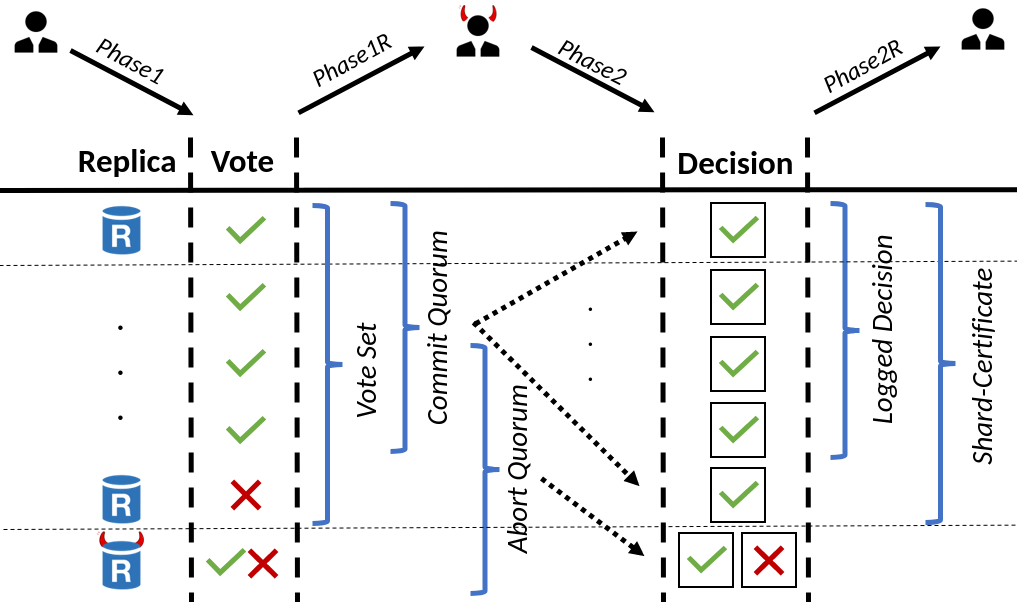
\includegraphics[width= 0.5\textwidth]{./figures/Nom2.png}
\end{center}
\caption{Validation Nomenclature, Slow-Path. Note, that a byzantine client may equivocate Phase2 decisions by including Commit and Abort Quorums respectively. Byantine replicas may store multiple votes and decisions.}
\label{fig:FigureSP}
\end{figure}

\subsubsection{Correctness}
We show, that a \textit{logged} decision is final:
\begin{theorem}[Saf]
A logged decision is durable, and there can ever exist \textbf{at most one} logged decision.
\end{theorem}
\begin{proof}
See TR.
\end{proof} 

Note, that since replicas never change their decision, it is possible for there to never be any logged decision if a byzantine client equivocated its Slow-Path Quorums. In order to reconcile this, we design and discuss a recovery mechanism in section X which relaxes the requirement on persisting a decision.  


\begin{theorem} 
Indicus maintains \textit{Byzantine-Serializability}.
\end{theorem}
To prove that this is the case, we show that for any two conflicting transactions, at most one can be committed.
\begin{proof}
See TR.
\end{proof}

\begin{theorem} 
Indicus maintains Byzantine Independence in the absence of network adversary.
\end{theorem}

We show, that once a Client submits a transaction for validation, the result cannot be unilaterally decided by any byzantine participant, be it client or replica.
\begin{proof}
See TR.
\end{proof}
%-------------------------------------------------------------------------------
\subsection{Writeback}
%-------------------------------------------------------------------------------



%-------------------------------------------------------------------------------
%\subsection{Granting Liveness}
%-------------------------------------------------------------------------------
\sys operates under the premise that clients experience progress indepentently - there exists no shared notion of system progress. Byzantine clients, may bring execution, validation or writeback to a halt for their own transactions: they may stall during all phases, or equivocate during validation logging, causing replicas to diverge on decision values (Commit/Abort) and thus prohibiting the generation of shard-certificates. When all transactions are commutative this phenomenon requires no action: Any client \textit{chooses} whether to adhere to the protocol and experience progress, or not. However, when transactions depend on each other, either explicitly by claiming dependencies on uncommitted write), or implicitly through read-write conflicts, liveness is no longer independent. For instance, a dependency that does not progress may cause the dependent to block indefinetely, while an uncommited, but insufficiently replicated, write might cause consecutive read transactions to abort.
In order to allow clients to safely intertwine their fate with concurrent transactions, \sys must provide clients the tools reclaim their own liveness. We define Liv: 
\begin{theorem}[Liv] 
Every transaction that a correct client is \textit{interested} in eventually completes.
\end{theorem}

Intuitively, correct clients may enjoy this progress property if they can reliably obtain shard-certificates as any client can conduct the writeback phase. To achieve this, we must relax the requirement that replicas may never alter their decision, while preserving Theorem Saf.

A naive solution that allows any client to drive another clients protocol is problematic, since \textit{interested} clients could concurrently make inconsistent decisions, thus inhibiting progress. Likewise, coordinator election across client is undesirable as there may exist an unbounded number of electable byzantine clients that may not constructively aid in reconciliation. In \sys we circumvents this by letting concurrent clients replay non critical sections of the protcol, while delegating critical responsibility to the bounded replica set. Concretely, we design a mechanism to endorse a dedicated \textit{Fallback} replica responsible for reconciling diverged replica decisions. Since the number of faulty replicas is bounded, at most $f+1$ leader elections are necessary to make progress when the network is synchronous. \sys challenge is to guarantee a live round-robin election while keeping clients responsible for their own progress. We remark, that in an asynchronous network, deterministic leader election might not be possible  \cite{fischer1985impossibility}.  \fs{no non-randomized protocol can reach agreement in an async setting. (randomized exceptions: BenOr, Honeybadger, BEAT)}.

On a high level, the recovery mechanism operates as follows: \textit{Interested} clients attempt to run the validation protocol themselves. If a client suspects decision divergence, it issues a \textit{Fallback invocation} request, electing a \textit{Fallback} replica that reconcile decisions. Such recovery protocol is reminiscent of \textit{view-changes} in traditional BFT SMR protocols, but differs in two core aspects: a) While control changes between fallback replicas (leaders), the protocol is still client driven and linear in complexity, and b) The fallback mechanism impacts only the ongoing transaction. Independent concurrent transactions are unaffected. Figure \ref{fig:FigureFBnom} shows an example scenario requiring reconciliation, and gives on overview of the  Fallback protocol message pattern.

\begin{figure}
\begin{center}
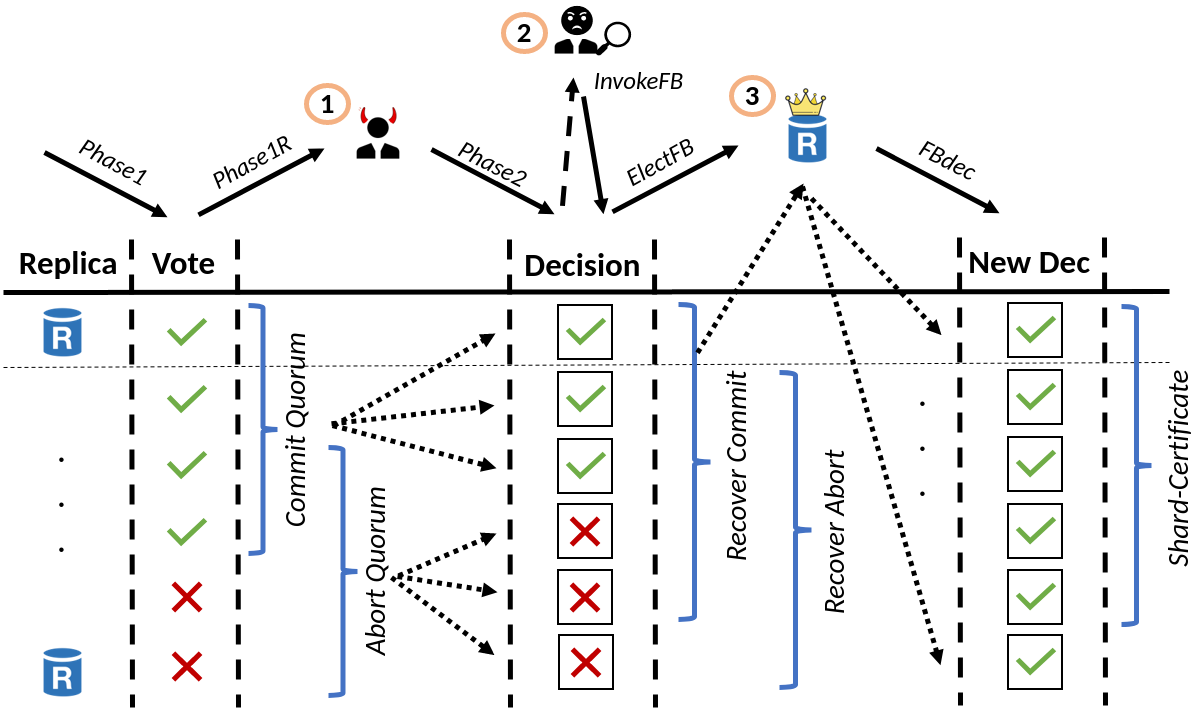
\includegraphics[width= 0.5\textwidth]{./figures/FBNom.png}
\end{center}
\caption{Fallback Scenario. 1. A byzantine client equivocates decisions. 2. An interested client invokes a Fallback Replica (FB) election. 3. A correct FB reconciles a single decision.}
\label{fig:FigureFBnom}
\end{figure}


Below, we detail the protocol by following a transactions life cycle. To start the protocol we assume an \textit{interested} client is in possession of the respective transactions $Prepare$ request, signed by the orignial issuer. This information may be obtained during the validation of the clients own transaction, either as full dependency or conflict. 
%%%%%%%%%%%%%%%%%%%%%%%%%%%%%%%%%%%% WRITEBACK HAS ALREADY HAPPENED


%%Cut the protocol re-iterations?

\fbox{\begin{minipage}{23em}
\textbf{(1: C $\rightarrow$ R)}: Client issues Prepare request and inquires current protocol state.
\end{minipage}}\\
An interested client broadcast a message $Backup-Phase1 \coloneqq (TX.Phase1, CID)$ to all replicas in \textit{InvolvedShards} of the transaction. \\
\fbox{\begin{minipage}{23em}
\textbf{(2: R $\rightarrow$ C)}: Replica marks Client as interested and returns its state.
\end{minipage}}\\
Replicas execute an un-seen $Phase1$ (see Validation, step 2), and reply with its vote. Otherwise, a replica replies with its current decision value and the corresponding view ($Phase2R$), or, if not existant, with its origninal vote ($Phase1R$), and lastly, its current view.\\
\underline{Finalized decisions:} If a replica has already received a Writeback message for a transaction it ignores all Fallback related client requests and simply returns the decision and corresponding certificate. An intersted client can return to the Writeback phase immediately and forward the response.\\
\fbox{\begin{minipage}{23em}
\textbf{(3a: C $\rightarrow$ R)}: A client receives the necessary information to proceed to Writeback.
\end{minipage}}\\
A client either a) receives a Fast-Path threshold of $Phase1R$ messages, or b) receives sufficiently many matching (in decision and view) $Phase2R$ messages to assemble a shard-certificate. \\
\fbox{\begin{minipage}{23em}
\textbf{(3b: C $\rightarrow$ R)}: A client needs to go Slow-Path or observes inconsistency and requires assistance for resolution.
\end{minipage}}\\
If a client receives insufficient $Phase2R$ replies to return, the client itself broadcasts $Phase2$ messages using the received $Phase1R$ or $Phase2R$ responses as proof in order to log a decision. If instead, a client receives inconsistent $Phase2R$ replies (either decision or view), it invokes a fallback election, broadcasting a message $InvokeFB \coloneqq (TxID, CID, \{view\}_R$ that includes a Quorum of replicas' current views.
Inconsistent replies from the same view $v$ additionally constitute a Proof of Misbehavior (PoM) for the issuing client or replica. \\
\fbox{\begin{minipage}{23em}
\textbf{(4a: R $\rightarrow$ C)}:  Replicas receive $Phase2$ messages and replies with decision
\end{minipage}}\\
A replica buffers requests until the orginial client timer expires, and, upon expiration, adopts the decision if it has stored none. It returns a corresponding $Phase2R$ message. \\
\fbox{\begin{minipage}{21em}
\textbf{(4b: R $\rightarrow$ R(FB))}: Replicas receives Fallback invocation and starts election
\end{minipage}}\\
If a replica receives an $InvokeFB$ message and the original client has timed-out it attempts to elect a new \textit{Fallback replica}. To do so, it follows the \textbf{View Change Rules} and adopts new view $current.view = v+1$ if $v \geq current.view$. 
Replicas send an $ElectFB \coloneqq (TxID, decision, current.view)_R$ to replica $current.view + TxID \% n$. \\
\underline{\textbf{View Change Rules:}} \one Replicas only adopt a view $v+1$ if the view set includes $3f+1$ votes from view $v$. \textit{Vote subsumtion:} A view $v$ may count as a vote for all $v' \leq v$. \two Replicas that lag behind, may safely skip ahead to the maximum view $v$ present $f+1$ times, since, by induction, $\geq 3f+1$ replicas must have claimed to be in a view $\geq v-1$. Thus, any possible divergence can be reconciled in a single step, as there must exist a view $v' \geq max(correct.views) -1 $ for which at least $f+1$ correct votes exist in any Quorum of $4f+1$ votes.\\
\underline{Additional subtlelties:} Replicas enforce exponential time-outs for new elections. In absence of correct interested clients, byzantine clients may invoke fallback elections at a subset of replicas, thus inhibiting true election and skipping select replicas' terms. To avoid artificially increased timeouts and non-skipping candidates, replicas may forward the $ElectFB$ message to all other replicas. Replicas that receive $f+1$ forwarded messages, adopt larger views, and forward the $ElectFB$ message themselves, thus ensuring election for each view.
\footnote{This optimization is not necessary for "theoretical" liveness. To avoid unecessary all-to-all communication, it may only be enforced for views $v > T$, where T is a system hyperparameter }\\
\fbox{\begin{minipage}{21em}
\textbf{(5: R(FB) $\rightarrow$ R)}:  Fallback aggregates and echos election messages.
\end{minipage}}
The Fallback replica considers itself elected upon receiving a Quorum of $4f+1$ ElectFB messages. It then uses this set of messages to reconcile a decision. It broadcasts a message $FBdec \coloneqq \langle RID, dec, view, \{ElectFB_r\} \rangle_R$, including proof for the new decision. \\
\textbf{Decision Reconciliation Rule:} \textit{$dec_{new}$ $=$ maj(\{Elect.decision\})}. If a logged decision exists (implies that a shard-decision might exist), any Quorum of $4f+1$ Elect messages is guaranteed to contain $2f+1$ matching decisions (a majority). Otherwise, an arbitrary decision qualifies since at least one correct replica must have agreed to it.\\
\underline{Additional subtlelties:} The attentive reader may notice that Elect messages do not include a corresponding view. Decisions need not match in views: By the Decision Reconciliation Rule, if there ever existed a logged decision $d$ with matching views, then all future $dec_{new} = d$.\\
\fbox{\begin{minipage}{21em}
\textbf{(6: R $\rightarrow$ C)}:  Replicas echo decision to interested clients
\end{minipage}}
Replicas receive a $FBdec$ message, adopt $decision = (FBdec.dec, FBdec.view)$ and $current.view = FBdec.view$ if $FBdec.view \geq current.view$, and forward the respective decision to all interested clients. Replicas that time out waiting for a $FBdec$ message proactively forward their current view to all interested clients. \\
\fbox{\begin{minipage}{21em}
\textbf{(7: C}: A client starts Writeback phase or restarts Fallback invocation
\end{minipage}}
An interested client returns to the Writeback phase upon receiving sufficiently matching decisions. If it times out, or receives inconsistent decisions it inquires a new set of current views and re-starts Fallback starts a new broadcast $InvokeFB \coloneqq (TxID, CID, \{view\}_R$.\\
\underline{Additional subtlelties:} A correct client \textit{expects} to receive $4f+1$ matching decisions and will continue to wait for decisions from the same view up to a timeout. Eventually a logged decision must exist and time-outs grow enough to guarantee a client will receive a shard-certificate. \fs{In section X (optimization) we discuss a practical optimization: Async extra phase.}\\
%%%%%%%
Given synchrony, any correct client that follows the Fallback protocol experiences \textit{Liv}. This follows straightforward from the eventual existance of a correct Fallback replica (at most $f+1$ elections) that reconciles all correct replicas. For any transaction, an interested correct client will eventually receive a shard-decision, and hence the transaction will complete.

We point out that steps 1, 2a, 3 and 4a simply correspond to the normal validation protocol. In order to avoid (multiple) \textit{interested} clients interfering too soon and causing unecessary divergence, we grant the original client an initial window of immunity.\footnote{Note, that it is irrelevant which client issues the $Phase1$ message. Therefore, we enforce the timeout window only for explicit logging ($Phase2$).} The orignial client is an interested client by default - a correct client that loses autonomy will, if necessary, elect a \textit{Fallback} itself. 

When depending on slow or byzantine transactions, clients may have to incur addtional latency in order to maintain liveness. On the flipside, when a clients fate is independent from other transactions, it is unaffected by concurrent slowdowns. 

%-------------------------------------------------------------------------------
\section{Further optimizations}
%-------------------------------------------------------------------------------


\fs{the current writeback might be unecessary to explain, since we implement the below anyways... Perhaps merge writeback and this subsection}
\par \textbf{Shard Logging} When transaction execution touches multiple shards validation can incur redundant explicit logging overhead. When a Slow-Path is necessary to arrive at a logged decision on S different shards, bandwith is wasted. Consider an example in which $S-1$ shards attempt to log the decision Commit, while a single shard attempts to log an Abort decision. If the latter shard succeeds, the effort of the remaining shards was in vain. \fs{Moreover, logging is always bottlenecked by the slowest shard. }
The culprit of this phenomenon is the delayal of Two-Phase-Commit (2PC) until the Writeback phase. By preemptively making a 2PC decision \textbf{before} logging we can avoid this redundancy. We remark, that even when when all shards agree on a decision, this saves redundant coordination. \fs{This does not work for Atomic Broadcast! In AB, the voting only happens AFTER the tx has already been logged (i.e. the order has been durably replicated)}

Concretely, we designate \textbf{one} involved shard as \textit{logging Shard} $=$ \textit{involvedShards[TxID \% |involvedShard|]}, while all other shards remain responsible only for Voting. \changebars{}{The logging Shard can be determin via a determinsitic function over the \textit{involved Shards}. A simple load balanced solution may select $loggingS = involvedShards[TxID \% |involvedShard|]$}. \changebars{}{Figure \ref{fig:SingleShardOpt} shows a comparison and the revised structure. dont use this figure in actual paper} In order to log a decision, Phase1R Quorums \fs{aka shard votes} from all involved shards are required. We modify step 3 of the Validation protocol accordingly:

\fbox{\begin{minipage}{21em}
\textbf{Validation (3: C)}: Client waits for vote replies from all involved Shards.
\end{minipage}}
A client aggregates a per-shard decision for each shard according to the \textit{CommitQuorum} rule. If all shard-decisions are Commit, it attempts to log a Commit decision by sending $Phase2 \coloneqq (TxID, Commit, S \times \{CommitQuorum\}$ to all replicas in the designated logging Shard. If a single shard-decision is Abort, it stops waiting for other shard-decisions and attempts to log an Abort decision by instead sending $Phase2 \coloneqq (TxID, Abort, AbortQuorum)$. 

\underline{Additional subtlelties:} A client can go Fast-Path and return to the Writeback phase immediately only if Fast-Path Quorums were received for all shards. 

The remaining Validation protocol proceeds identically to the multi-shard version. Notice, that when only a single shard is involved, no adjustments were made. The Writeback phase instead, may proceed with just the single certificate from the logging Shard


The Fallback protocol is adjusted accordingly: A fallback replica need (and can) only be elected on the logging Shard, simplifying reconciliation and reducing the cost for interested clients. 
To further reduce unecessary load, a client may attempt to first inquire whether decisions exists at the logging shard (Fallback protocol step 1 \& 2), before sending $Rec-Phase1$ messages to all shards in order to gather votes itself (Fallback protocol step 1). 

\iffalse
\begin{figure*}
\begin{center}
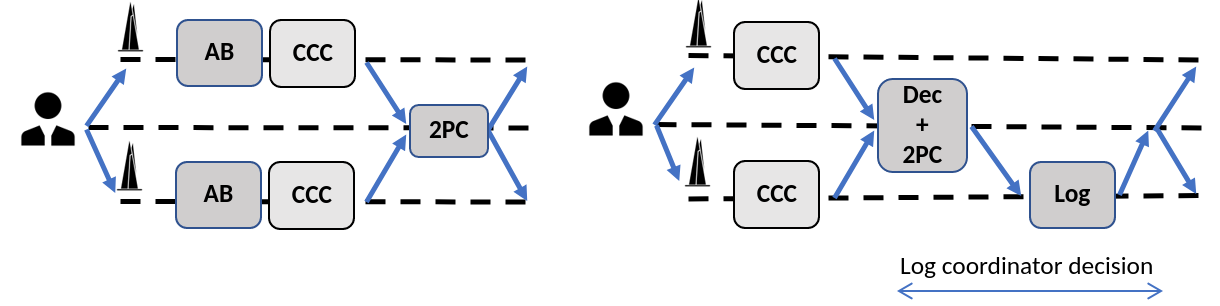
\includegraphics[width= \textwidth]{./figures/SingleShard.png}
\end{center}
\caption{Single Shard Optimization}
\label{fig:SingleShardOpt}
\end{figure*}
\fi

\par \textbf{Batching}
To amortize cryptographic overheads we introduce message batching. However, unlike leader based systems, in \sys there exists no central sequencer that may batch request. Instead, \sys implements message batching at the replicas by batching $b$ messages, generating a merkle tree \cite{merkle1987digital}, and signing only the root hash, thus reducing signing overheads from $O(b)$ to $O(1)$ per batch. The merkle hash tree allows replicas to respond to individual clients by including only the single client-addressed message and $log(b)$ additional hashes. We note, that since replicas receive requests out of order, their batches are not consistent. Consequently, a client must aggregate hashes and signatures from different merkle trees to forward as proofs (Phase2 and Writeback messages include $O(n)$ signatures and hashes) .
In order to reduce verification overheads from $O(n*b)$ to $O(n)$, replicas cache previously verified signatures by storing a mapping from signature to merkle hash roots. For following message verifications, a replica can omit de-computing the signature, and must only re-compute and compare the merkle root based on the hashes included in the proof.

\iffalse
- amortize signature cost
- unlike leader based, there is not an obvious sequencer to batch
- instead we batch signature generation at replica. Because they can be out of order these batches are different. Also do not want to send the whole batch (b* hashes) to every client. Instead we use a merkle tree and send only the root sig + log(b) hashes. (this means that we had to do 2*b hashes during signature gen, but we only do b*log(b) hashes at generation instead of b*b. OR: could send whole batch of  messages --> huge message + hashing cost..
- Cache already validated signatures at replicas and only recompute the hash to see whether it matches. This reduces verification by a factor of b (effectively only verifying for the first message from the batch).
\fi

\par Other non impelmented opts: in TR.

%
%\fs{whole section probably needs to fit in max 2 pages}

\sys{}'s execution protocol has three goals: 1) to offer clients an interactive transaction interface \fs{too obvious?}, 2) to be scalable, and 3) to maintain independent operability \fs{and Byzantine independence, Serializability}.

\sys{} achieves these goals by combining optimistic client-side execution with an aggressive, but Byzantine resilient, concurrency control (CC) scheme that maintains Byz-Serializability. 
\iffalse
 \la{We seem to have already made this points in the intro tio the section} \changebars{}{\sys leaves clients responsible for executing the transactions they submit, and allows every client, in parallel, to execute arbitrary interactive transactions using read RPC's, instead of submitting stored procedured that must be ordered and executed by replica servers.}  
 \fi By relying on optimistic rather than pessimistic CC schemes such as 2-phase-locking (2PL), \sys{} forgoes costly coordination to acquire locks, and sidesteps the concern of Byzantine clients refusing to relinquish locks.

\iffalse
\la{I would just remove the following} 
\changebars{}{Before we detail Indicus’s transaction processing and validation mechanism, we first discuss the CC that Indicus imple- ments as the latter are functions of the precise CC requirements.}
\fi

\subsection{\sys{}'s Concurrency Control}

%%% Explain MVTSO itself only briefly. Then explain how we make it for for byz
% 1) bound timestamps, 2) make writes visible late only, 3) only allow f+1 matchin uncommitted writes, 4) read timestamps
%Afterwards: explain execution interface. After that explain validation check. Then have overarching example
\iffalse
% we need to change a few things:
0) timestmap bound
1) Read validity
2) deferred writes
3) read uncommitted
4) byz read timestamps (read lock implies you had access control, at that point it is no different than issuing a tx and completing. But we do not want to give the power to abort for no reason. It should be traceable.
\fi

\fs{fig doesnt make so much sense before reading the whole thing} \fs{cut this preamble?}
Figure \ref{fig:MVTSOEX} shows an example trace of \sys operational behaviors under different request processing orders (assume $f=1$) that we use to guide the remaining outline.

\begin{figure*}
\begin{center}
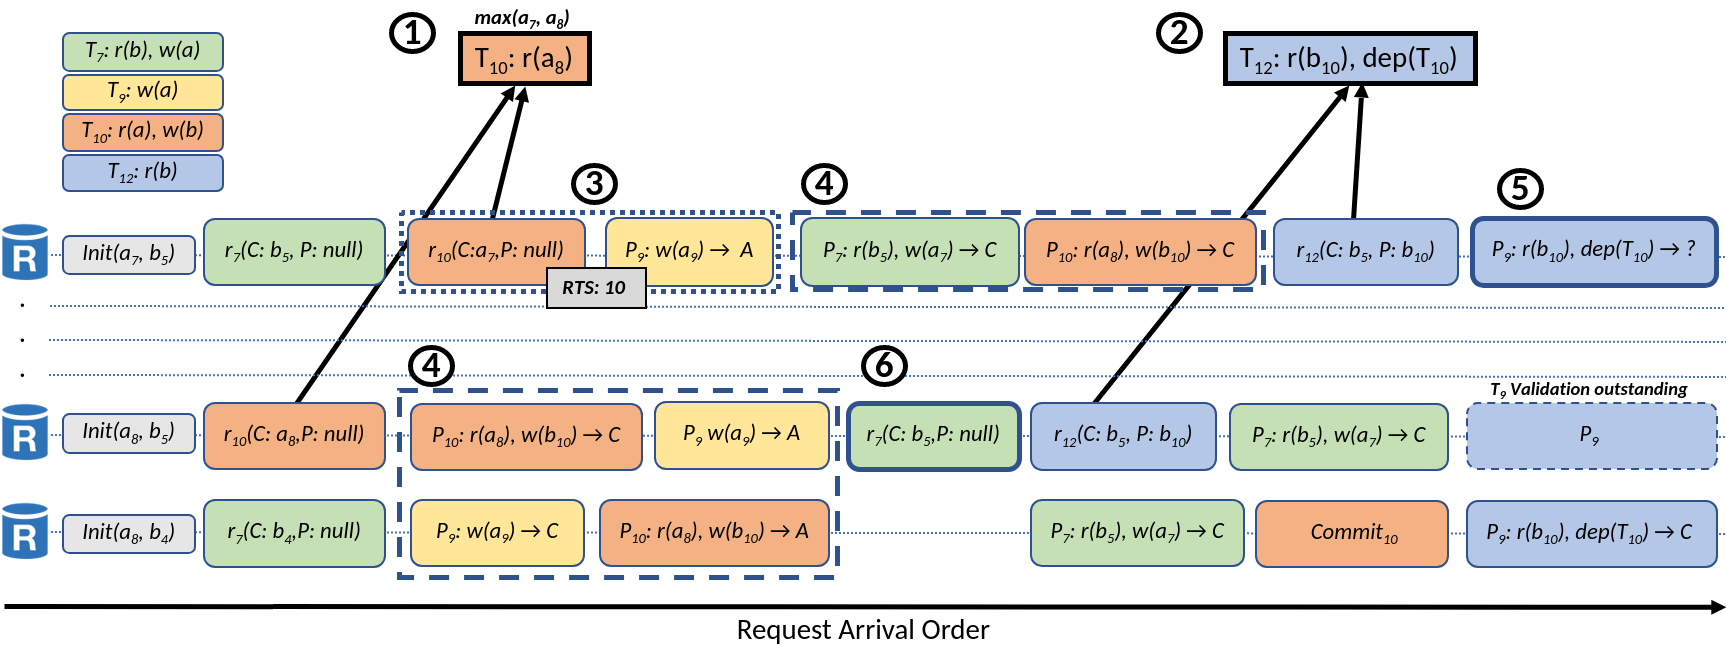
\includegraphics[width= \textwidth]{./figures/MVTSOLargeFont.png}
\end{center}
\caption{\emph{MVTSO behavior for different replica processing orders}. $r_x(C : a_y ,P : a_z)$ denotes that transaction $T_x$ (x being the timestamp of a transaction in this example) reads the version $y$ of object a written by committed transaction $T_y$ and version $z$ from tentative prepared transaction $T_z$. $P_x(RS,WS,DEP)$ denotes a transaction $T_x$'s prepare request (i.e. the validation check) for respective ReadSet (RS), WriteSet (WS) and Dependenc Set (DEP), and $\rightarrow C / A$ denotes the local replica validation outcome (Commit/Abort).} 
\label{fig:MVTSOEX}
\end{figure*}

\par \textbf{MVTSO.} Our starting point is Multiversioned Timestamp Ordering (MVTSO), a concurrency control scheme which prescribes a serialization order by assigning a speculative timestamp \textit{before} execution \cite{bernstein1983multiversion, reed1983implementing, su2017tebaldi}. In MVTSO, read operations return the latest written version smaller than the readers' timestamps. Respectively, writers attempt to create new versions at their timestamp, but must abort if a higher timestamped read would have "missed the write" by reading a prior version. A transaction may commit only, if all read-write dependencies have committed.

\iffalse
\fs{cut the whole following paragraph?} \la{Yes, I would cut it} This allows us to a) only classify concurent read/write operations as conflicting if their execution results violate the timestamp order (Fig. \ref{fig:MVTSOEX}: 4 bottom), and b) avoid write/write conflicts alltogether. 
When speculative execution results match the pre-defined timestamp order, no aborts are necessary (Fig. \ref{fig:MVTSOEX}: 4 top). \sys{}'s challenge is therefore to a) assign appropriate timestamps and b) coordinate execution in a way that maximizes such coherence; the presence of Byzantine participants (clients/replicas) complicates this.

In MVTSO, reads operations return the latest written version smaller than the readers' timestamps, while writers attempt to create new versions at their timestamp, but must abort if a higher timestamped read would have "missed the write" by reading a prior version. A transaction may commit only, if all read-write dependencies have committed.
\fi

When \sys{}'s speculative execution results match the pre-defined timestamp order, no aborts are necessary (Fig. \ref{fig:MVTSOEX}: 4). \sys{}'s challenge is therefore to a) assign appropriate timestamps and b) coordinate execution in a way that maximizes such coherence; the presence of Byzantine participants (clients/replicas) complicates this.

\par \textbf{Byzantine resilience.} Read operations in \sys have the following sub-goals: \one Correct clients should read valid data, i.e. experience read integrity, \two Correct clients should read fresh data, i.e. minimize staleness and hence maximize commit chance, and \three Reads must provide the context necessary to potentially complete observed write state. 
Clients validate the integrity of reads by requiring replicas to provide a proof of validity, which consists of a set of signatures confirming committment, or if not yet existant, a set of  $f+1$ replica's tentative commit endorsements \fs{maybe cut this second part, since it will become redundant}. Moreover, to guarantee that clients do not read maliciously stale data from their local replica, \sys encourages clients to read the latest version across $\geq f+1$ replicas (Fig. \ref{fig:MVTSOEX}: 1,2).
Avoiding Byzantine influence comes at a cost: Read operations require a synchronous, potentially WAN \fs{or just remote - i.e. not local}, rountrip. 

MVTSO intuitively synergizes well with \sys{}'s potenially WAN remote reads as reading from a fixed timestamp helps speculative readers observe consistent snapshots, even when execution is long and consequently interleavings are frequent (Fig. \ref{fig:MVTSOEX}: 6). \fs{at the price of experiencing serializability instead of strict serializability - that is only the case if your timestamps are outdated}.

While we assume that clocks are loosely synchronized across correct participants, Byzantine participants may diverge arbitrarily and propose excessively high timestamps. A simple solution is to bound time-stamps by querying the median time from a Quorum of replicas and including replies as proof \cite{bazzi2004non, bazzi2018clairvoyant}. To side-step the additional overheadd that a dedicated timestamping phase incurs, we compromise by allowing clients to optimistically select their own timestamps, but reject request timestamps above a threshold at all correct replicas, thus incentivising clients to select bounded, close to real-time, timestamps. 

In traditional MVTSO, writes become visible to successive, higher timestamped, reads immediately. However, in the presence of Byzantine clients this is undesirable, as it allows clients to issue write operations without the intention of ever committing a transaction. Thus, any correct clients' read that observes, and consequently depends on a Byzantine clients write may be blocked indefinitely.
%Allowing other clients to preemtively commit outstanding write operations is infeasible, as the remaining transaction procedure is known only to the issuing client, while conceiding pessimistic abort permission empowers Byzantine participants to obstruct any correct clients' writes. 
\sys reconciles this dilemma by deferring all database updates until execution is complete and the client prepares the transaction for commitment. 
% Concretely, \sys clients buffer all write operations, and submit them only when attempting to commit the transaction, thereby enabling other \sys client to orderly complete Validation and Writeback steps.\\
\la{This needs to be better explained} \fs{took a pass:}
Clients in \sys distinguish explicitly between writes \textit{committed} across all involved shards and tentative writes \textit{prepared} at a single shard: While clients accept all verifiable \textit{committed} version from a single replica, they accept \textit{prepared} versions only when endorsed by $f+1$ replicas. This ensures that a) at least one correct replica believes that the write can commit, and hence is worth observing, and b) that Byzantine replicas and clients cannot collude to violate Byzantine independence by reactively inventing versions. \fs{such invented transactions could be designed to be guaranteed to abort: I.e. by claiming to have read an out-dated version. The write versions could be engineered to be perfectly at the bound of the read timestamp, such that it is guaranteed to be chosen}\\
Finally, \sys replicas evaluate writes for conflicts by maintaining a Read Timestamps (RTS) for each locally processed read (Fig. \ref{fig:MVTSOEX}: 3). While this allows un-prepared reads to elicit external effects, these affect only concurrent transactions with smaller timestamps and can be bypassed by re-trying a transaction. To nonetheless limit recurrent abuse, we discuss a personalized lease mechanism to limit Byzantine influence in section Y.z (Optional Modifc). \fs{or just do it here in 1-2 sentences. We do not implement this though.}



\subsection{Execution interface}
Client applications execute transactions via the following interface. A TX object \textit{TXObj $\coloneqq$ (SeqNo, ClientID, InvolvedShards, ReadSet, WriteSet, Dependencies)}, records the state necessary for Validation.

\iffalse
\begin{figure}
\begin{center}
\includegraphics[width= 0.5\textwidth]{./figures/TxState.png}
\end{center}
\caption{Transaction execution state}
\label{fig:Txstate}
\end{figure}
\fi

\textbf{Begin()} A client begins a transaction by optimistically choosing a timestamp \textit{TS $\coloneqq$ (Time, ClientID)} that defines a total serialization order across all clients.  \\
\textbf{Write(key, value)}. A client buffers the write: \textit{WriteSet = WriteSet $\cup$ (key, value)}\\
%%%%%%%%%Read protocol%%%%%%%%%%%
\textbf{Read(key, TS, RQS)} 
If \textit{key $\in$ WriteSet} a client returns the buffered write value. Otherwise, the client conducts a remote read for given hyperparameter Read Quorum Size (RQS):

\fbox{\begin{minipage}{23em}

\textbf{1: C} $\rightarrow$ \textbf{R}: Client sends read request to Replicas
\end{minipage}}\\
%Improve RQS formulation
A client broadcasts a read request  $m = (Read, key, TS)_c$.
\iffalse
 to $RQS$ different replicas. Note, that in order to guarantee $\geq RQS$ replies a client might need to send up to $f$ additional requests to compensate for unresponsive/faulty participants ($max(|Replies|) \leq n-f$). 
\fi
\fs{Optimization: A client sends only to RQS+f to receive RQS many replies}

\fbox{\begin{minipage}{23em}
\textbf{2: R} $\rightarrow$ \textbf{C}: Replica processes client read and replies
\end{minipage}}\\
A replica authenticates the client\footnote{Byzantine replica may ignore read access control. Solving this problem is beyond the scope of this work; we defer to existing solutions \cite{basu2019efficient}.}, and enforces a local timestamp threshold. \fs{this can probably be shortened:} It returns a signed message \text{$\langle \textit{ReadReply, Committed, Prepared} \rangle _R$}, where $Committed \coloneqq (value, version, proof)$ represents the value-version pair with largest committed write version smaller than TS and a proof of commitment,  and $Prepared \coloneqq (value, version, TxID', deps)$ the respective largest uncommitted value-version pair, the associated transaction ID, and the latter transactions potentially uncommitted read-write dependencies. Moreover, a Replica stores a new read timestamp (RTS) for the key: $RTS(key) = RTS(key) \cup TS$ (Fig. \ref{fig:MVTSOEX}: 3). 
\fs{a replica may include a set of prepared values to increase likelihood of client receiving f+1 matching}

\fbox{\begin{minipage}{23em}
\textbf{3: C} ($\rightarrow$ \textbf{R}): Client receives read replies 
\end{minipage}}\\
A client waits for $\geq RQS$ read replies and chooses the biggest valid result \textit{(value, version) $= max_{valid}$(\{Committed\},\{Prepared\}} (Figure \ref{fig:MVTSOEX}: 1,2). A \textit{Committed} tuple is valid, if the proof confirms commitment, wheras a \textit{Prepared} is valid iff there exist $f+1$ matching \textit{Prepared$_r$}. The client adds the version to its read set \textit{ReadSet = ReadSet $\cup$ (key, version)} and additionally claims a dependency if it was a \textit{Prepared} version: \textit{Dep = Dep $\cup$ \{f+1 $\times$ Prepared$_r$ \}} . 

\fs{la: finds the use of commit in both exec and validation confusing. Is it unclear that this refers to application here?}
\textbf{Commit()} A Client terminates its execution, and computes a unique transaction identifier based on final execution object and its timestamp: $TxID \coloneqq (H(TxObj, TS)$, thus preculding Byzantine participants from equivocating transaction contents. It then initiates the Validation Phase by issuing a 2PC-Prepare requests to each involved shard.
%What if a byz doesnt send to all involved shards? It will be visible on some shard and hence an correct client can obtain the full TX. See Hierarchical IDS in Protocol.tex

\textbf{Abort()} A client terminates execution, and broadcasts a request to release all acquired Read Timestamps (RTS). Since writes in \sys are deferred, no other rollback action is necessary.


We briefly discuss some implications of the choice of Read Quorum Size (RQS). Following cases may be distinguished: \one \textbf{$RQS = 1$} A client may read committed data from just \textit{trusted} replica (at the risk of reading stale data) to reduce execution latency and consequently minimize conflicting interleavings. \two \textbf{$RQS \geq f+1$} \sys{}'s recommended minimal mode of operation. While side-stepping maliciously stale reads, it is still possible to read (arbitrarily) stale data due to replica inconsistency, caused by either asynchrony or partial transaction replication by a Byzantine client.
\three \textbf{$RQS \geq \frac{n+f+1}{2}$} When reading from a Quorum of sufficient size to overlap with any Validation Quorum (ref section Validation) in at least one correct replica, a client guarantees, that no more \textbf{additional} (beyond previously observed) conflicting writes can be admitted, since such a Quorum of acquired RTS acts as a read-lock. 

\iffalse
Trusting only $f+1$ matching prepared writes has the beneficiary side effect of allowing us to include only transaction identifiers as dependencies, rather than the full transaction, since it is guaranteed that at least one correct replica has stored the transaction. Thus, in the failure free scenario, where clients need not complete transactions $in Dep$, \sys minimizes the meta-data overhead that the recovery protocol imposes.
\fi

We remark that, consistent with Byz-Isolation, \sys allows Byzantine clients to fabricate and (permissibly) submit arbitrary reads; Byzantine clients may \textit{choose} whether to read legal, or even real data.  \sys does, however, enforce that Byzantine clients cannot (undetectably) fabricate dependencies by requiring a proof of $f+1$ matching prepared writes. This precludes Byzantine clients from indetectibly stalling their own transactions and consequently obstructing liveness for consecutive descendant (second degree...) dependencies.
Furthermore, this allows \sys to include only transaction identifiers as dependencies, rather than the full transaction, thereby minimizing the common path overhead. The full transaction can be acquired from an correct replica when necessary. We discuss how to complete stalled or slow transactions in section Y (Granting Liveness).





%%-------------------------------------------------------------------------------
\subsection{Validation Phase}
%-------------------------------------------------------------------------------

In order to facilitate atomic committment across all shards involved in a transaction \sys clients invoke a Prepare request, inquiring each shard to validate the transaction for conflicts and cast a 2PC vote. Shards in \sys are replicated for fault tolerance.

\fs{idk where to put this and whether to mention at all - but we do want to state that there exists a version with 3f+1 (minimal replication degree) that implements the same ethos }
\sys comes in two different flavors, \sys{}3 and \sys{}5 respectively, that rely on varying replication degrees, but implement the same design. \sys{}3 requires $n=3f+1$ replicas \fs{, the minimum bound necessary for BFT SMR?,} per shard to guarantee consistency in the presence of $\leq f$ byzantine replicas. \sys{}5 reduces both latencies during failure free execution and complexity during recovery. \footnote{We believe that consortiums with high performance requirements or high replication degrees are respectively comfortable with paying for additional replicas or tolerating a lower fraction (1/3 vs 1/5) of failures}
For the simplicity of exposition we discuss \sys{}5 for the remainder of the paper, and defer to section X \fs{and/or TR} to describe differences in \sys{}3. In the following, we outline \sys 's execution (unaffected by replication degree), validation and writeback protocols.

The goals of the Validation phase are threefold: \one It must decide on a single, durable vote per-shard that maintains Byzantine Serializability (henceforth we refer to this as a \textit{shard-decision}), \two It should be leaderless, and not enforce unecessary ordering for commutative, non-conflicting transactions, and \three It must preserve independent operability. \fs{needs to refer to the fallback}

Satisfying these goals requires ovecoming several challenges. In order to maximize parallelism and embrace partial ordering, \sys allows replicas to process requests out of order. Consequently, replicas may temporarily diverge, and hence return different validation results. Such divergence must be reconciled in a way that maintains Isolation, but not overly conservatively in order to bound the impact of byzantine participants and maximize likehlihood to commit. \sys designates clients as validation coordinator for its own transactions, thus omitting a dedicated replica leader. %The respective protocol must tolerate client failures such as crashes, omission/stalling, equivocation, or replays and allow for consistent recovery. 

The Validation protocol can be broken down into two functionalities: Voting and Logging.
Since \sys replicas may process requests in different order, they must reach consensus on a joint  decision. To do so, they cast a vote for their local validation result, which are subsequently democratically aggregated into a decision. In the case of Indicus, the client acts as the transaction coordinator who aggregates and relays results (along with necessary evidence).
In order to maintain consistency in the presence of failures (no two honest replicas finalize different Commit/Abort decisions), this decision must be durable and unique, guaranteeing that a replay of any Writeback is idempotent. However, since a byzantine coordinator cannot be trusted to durably store a decision, nor could we retain liveness during a crash or partition, \sys demands clients to \textit{log} the decision at replicas before returning.
 

The voting step requires a single round-trip to all replicas, whereas the logging phase requires at most one round-trip \fs{in Indicus5 and at most two round-trips in Indicus3.}. When execution is fault- and contention free transactions can be committed on the \textit{Fast-Path} in a single-round trip as an explicit logging round is not necessary.


%%%%%%%%%% protocol
To describe how the protocol operates in detail we follow a single-shard transaction through the system:

\fbox{\begin{minipage}{23em}
\textbf{(1: C $\rightarrow$ R)}: Client sends Prepare request to all Replicas within the Shard.
\end{minipage}}\\
Upon deciding to Commit in the Execution phase, a Client initiates Validation by sending a message $Phase1 \coloneqq \langle Prepare, TxID, TX \rangle_{\sigma_c}$ to all Replicas.

\fbox{\begin{minipage}{23em}
\textbf{(2: R $\rightarrow$ C)}: Replica receives validation request, processes it and returns vote to Client.
\end{minipage}}\\
A replica validates Timestamp and Dependency integrity of the request. It then evaluates Read and Write Sets for Isolation conflicts against its local state using the MVTSO Concurrency Control Check (CCC), as shown in algorithm 1. It returns a message $Phase1R \coloneqq \langle TxID, vote \rangle_r$, and optionally evidence in case it voted to Abort.

\underline{Additional subtlelties}: 
A replica never changes its Voting decision, because re-execution could leave to different results. Once the MVTSO-Ceck completes (i.e. there are no blocking dependencies), a replica starts a timer to monitor the clients progress.

\fbox{\begin{minipage}{23em}
\textbf{(3: C)}: Client waits for vote replies.
\end{minipage}}\\
A client waits for at least $n-f$ ($4f+1$ in Indicus5) distinct replica votes, or more, up to a system specified timeout. 

\fbox{\begin{minipage}{23em}
\textbf{(3a: C)}: Client receives Threshold of matching votes and returns to application. Proceeds to Writeback
\end{minipage}}\\
In any of the following 3 cases, a client may short-circuit waiting for additional votes and omit a dedicated Logging round:
\begin{enumerate}
\item \textbf{$1$ Abort vote w/ Conflicting TX \& CommitCertificate}: A conflict with a commited transaction. The client validates the integrity of the CommitCertificate and returns the shard decision $(TxID, Abort, \langle ConflTX \rangle_{CC})$. 
\item \textbf{$3f+1$ Abort votes w/ Conflicting TX}: A conflict with a prepared, but not yet committed transaction. The client returns the shard decision $(TxID, Abort, \{\langle AbstainVote\rangle_r\})$. 
\item \textbf{$5f+1$ Commit votes}: No conflicts. The client returns the shard decision $(TxID, Commit, \{\langle CommitVote \rangle_r\}$
\end{enumerate}
Any of such Quorums forms a \textit{Shard-Certificate} and proves the decision. A client uses this Certificate to return to its application and issue the Writeback.

\fbox{\begin{minipage}{23em}
\textbf{(3b: C $\rightarrow$ R)}: Client receives divergent results and suggests a consistent decision to Replicas for Logging
\end{minipage}}\\
If a client does not receive the necessary thresholds of votes to return, it must continue on the \textit{Slow-Path}. To do so, it aggregates the votes according to following decison rule:
If there exists a $CommitQuorum \coloneqq \frac{n+f+1}{2}$ of Commit Votes, the Slow-Path decision is Commit, otherwise it is Abort.
A client broadcasts a message $Phase2 \coloneqq (TxID, decision)_c, \{\langle votes \rangle_r\}$.

\underline{Additional subtlelties}: A client forwards a Quorum of $\geq n-f$ votes to the replicas in order to prove the Slow-Path decision is consistent with Isolation guarantees. Note, that a byzantine client may equivocate the decision by relaying different Quorums.

\fbox{\begin{minipage}{23em}
\textbf{(4: R $\rightarrow$ C)}: Replicas receive, validate and echo decision
\end{minipage}}\\
A replica confirms that the Decision matches the Quorum by evaluating the decision rule itself and adopting the decision. It then returns the decision to the client by sending $Phase2R \coloneqq \langle TxID, decision \rangle_r$. Importantly, a replica never changes its decision.

\fbox{\begin{minipage}{23em}
\textbf{(5: C)}: Client returns shard-decision to application and proceeds to Writeback
\end{minipage}}\\
A client waits for a Quorum of $n-f$ matching $Phase2R$ messages. Such a Quorum forms a \textit{Shard-Certificate} and proves the decision. A client uses this Certificate to return to its application and issue the Writeback.

\underline{Additional subtlelties}: If a client equivocated, it will never receive a Shard-Certificate. An honest client however, is guaranteed to receive matching Phase2 replies. 

We consider a decision (Commit, Abort) to be \textit{logged} when it is possible for some Shard-Certificate to exist, i.e. as soon as the necessary certificate Quorums exists at some Replicas.
Figure \ref{fig:FigureSP} summarizes the relevant nomenclature.

\begin{figure}
\begin{center}
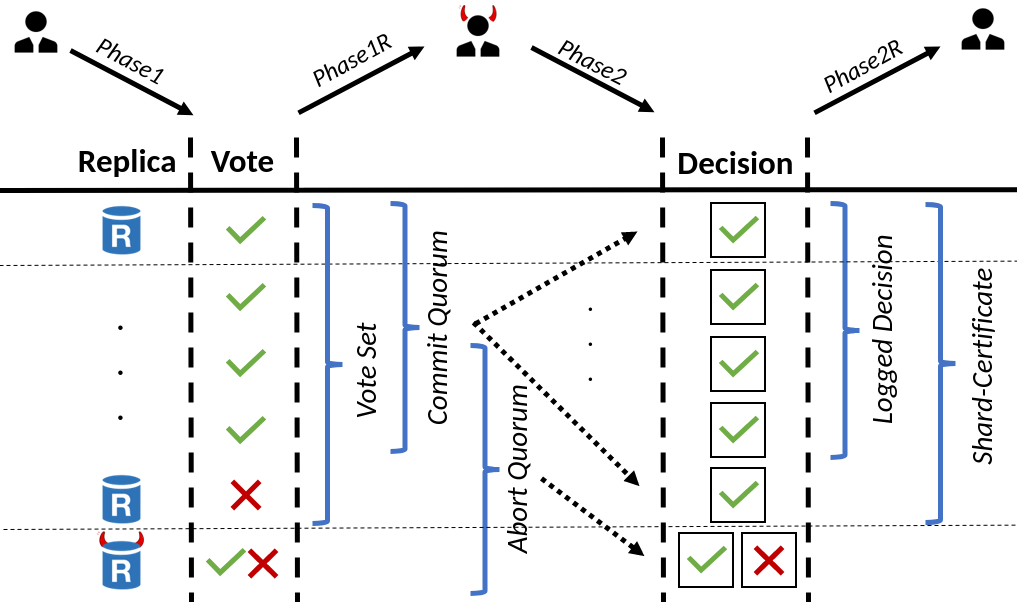
\includegraphics[width= 0.5\textwidth]{./figures/Nom2.png}
\end{center}
\caption{Validation Nomenclature, Slow-Path. Note, that a byzantine client may equivocate Phase2 decisions by including Commit and Abort Quorums respectively. Byantine replicas may store multiple votes and decisions.}
\label{fig:FigureSP}
\end{figure}

\subsubsection{Correctness}
We show, that a \textit{logged} decision is final:
\begin{theorem}[Saf]
A logged decision is durable, and there can ever exist \textbf{at most one} logged decision.
\end{theorem}
\begin{proof}
See TR.
\end{proof} 

Note, that since replicas never change their decision, it is possible for there to never be any logged decision if a byzantine client equivocated its Slow-Path Quorums. In order to reconcile this, we design and discuss a recovery mechanism in section X which relaxes the requirement on persisting a decision.  


\begin{theorem} 
Indicus maintains \textit{Byzantine-Serializability}.
\end{theorem}
To prove that this is the case, we show that for any two conflicting transactions, at most one can be committed.
\begin{proof}
See TR.
\end{proof}

\begin{theorem} 
Indicus maintains Byzantine Independence in the absence of network adversary.
\end{theorem}

We show, that once a Client submits a transaction for validation, the result cannot be unilaterally decided by any byzantine participant, be it client or replica.
\begin{proof}
See TR.
\end{proof}
%
\subsection{Validation Check}

Algorithm \ref{mvtso} shows the necessary validation check to preserve Byzantine-Serializability. 
Given a transactions prepare request the validation check returns an Abort vote if a conflict has been detected, and Commit otherwise. 
When execution results match the timestamp order, there are no conflicts (Fig. \ref{fig:MVTSOEX}: 4 top). For each read, a replica verifies that it has not voted to commit a conflicting write (Algorithm \ref{mvtso}, line 3-7). Conversely, for each write, a replica confirms that there exist no previously accepted reads (line 8-10), and no ongoing read transactions (line 11-12) that conflict. Fig. \ref{fig:MVTSOEX}: 4 shows both non-conflicting and conflicting interleavings.
If there are no conflicts, a replica tentatively \textit{prepares} a transaction, making its writes visible and evaluating future transactions against it for conflicts. Regardless of the outcome, a replica garbage collects all Read Timestmaps (RTS) associated with the transactions reads.
It then waits for necessary dependencies (uncommited writes that were read) to be resolved (Figure \ref{fig:MVTSOEX}: 5). We remark, that the concurrency control check is serialized and executed atomically for each transaction.

\begin{theorem}
The set of transactions for which the MVTSO-Check returns Commit is Byzantine-Serializable. 
\end{theorem}
\begin{proof}
See TR.
\end{proof}

\begin{algorithm}
\caption{MVTSO-Check(TX, TS)}\label{mvtso}
\begin{algorithmic}[1]
\If{\textit{$TS > localClock + \delta$}} %  || $TS < lowWM$ || $\exists d \in dep: d.TS < lowWM$} } dont mention garbage collection part here, it only confuses
\State \Return Abort
\EndIf

\For{\textit{$\forall key,version \in \textit{TX.RS}$}}
        \If{$ \exists TX2 \in Committed \cup Prepared: key \in \textit{TX2.WS} $ \newline
        \hspace*{2em} $\land \, version < \textit{TX2.TS} < TS$}  
          \State  \Return Abort, \textit{TX2, (TX2.CommitProof)}  
         \EndIf  
\EndFor

\For{\textit{$\forall key \in \textit{TX.WS}$}}
        \If{$\exists TX2 \in Committed \cup Prepared:$ \newline 
        \hspace*{2em} $\textit{TX2.RS[key].version} < TS < TX2.TS$} 
          \State  \Return Abort, \textit{TX2, (TX2.CommitProof)}
         
        \EndIf
        \If{$\exists RTS \in key.RTS: RTS > TS$} 
          \State  \Return Abort
       \EndIf
\EndFor
\State Prepared.add(TX) 

\While{$\exists d \in dep: d \notin CommitLog \cup AbortLog $)}
\State Suspend
\EndWhile

%structure it in a way that is better
\For{\textit{$\forall d \in dep$}}
		\If{$ d \in AbortLog $}
		\State	Prepare.remove(TX)
		\State \Return Abort, \textit{(TX2.AbortProof)}
		\EndIf
\EndFor
\State \Return Commit
\end{algorithmic}

\end{algorithm}

In order to perform the MVTSO-check, a replica maintains several data strucutres: \one It stores read timestamps, read versions alongside the multiversioned write stores for committed and tenative transactions respectively, to provide efficient evaluation of conflicts.
\two In order to confirm dependency outcomes, replicas log proofs for completed transactions in respective Commit and Abort Log sets, that together induce the ledger of all processed transactions. 
\three To avoid busy waiting when dependencies are not yet resolved, a replica temporarily suspends the MVTSO-check for the current transaction, allowing it to process other transactions pending validation. To facilitate this, it keeps track of an additonal transaction to dependents mapping that allows to identify and resume all suspended MVTSO-checks associated with dependents of a completing transaction.

\iffalse

\textit{Aside:} Consistent with our definition of Byzantine-Isolation, byzantine clients may issue ficticious Read-Sets comprised of arbitrary read versions and values. However, these have only limited external effect on concurrent writes. We distinguish two extreme cases: 1) $read.version \rightarrow 0$: This case is equivalent to simply reading stale data, and effectively reduces MVTSO to TSO as conlflicts are evaluated only on basis of the transaction timestamps (i.e. Abort write if: write.TS < read.TS). 2) $read.version \rightarrow read.TS$: In this case there are no conflicts as a write is never "missed" by a previous read.
\fi

In the following section we will show how to design a replicated validation scheme that upholds Isolation guarantees and reaches a single shard decision, even when replicas within a shard validate in different orders.

%%-------------------------------------------------------------------------------
\subsection{Consistent logging.}
%-------------------------------------------------------------------------------
Principles and challenges

protocol overview: pic

%%-------------------------------------------------------------------------------
\subsection{Writeback}
%-------------------------------------------------------------------------------



%\subsection{Multi-sharding}

and Multi-shard 2pc

- Optimization: Single shard logging

%%-------------------------------------------------------------------------------
\subsection{Failures}
%-------------------------------------------------------------------------------
- Fallback: election (only starts if not waiting on another dep to avoid early eviction), views, resolution, subtelties with mvtso (block because of dep), necessity even without dependencies. Interested clients, write-back multishard. garbage collection
- Fallback requires an extra round in order to learn about current views to start viewchange, but thats ok: Its co-function with learning about full TX, and checking for existing certificates. Timeout invocation is concurrent with p1 message.

%%-------------------------------------------------------------------------------
\subsection{Low Cost mode}
%-------------------------------------------------------------------------------
3f+1 if not defending against byz colluders
OCC if not worried about reads aborting


%-------------------------------------------------------------------------------
\section{Protocol}
%-------------------------------------------------------------------------------
Indicus comes in two different flavors, Indicus3 and Indicus5 respectively, relying on varying replication degrees. Indicus3 requires 3f+1 replicas per shard to guarantee consistency, the minimum bound necessary for BFT SMR. Indicus5 uses a higher replication degree of 5f+1 replicas, but in return brings down both gracious execution latency and complexity during uncivil executions. We argue, that unlike past system settings where a single authority strives to maintain the fewest amount of replicas necessary for cost considerations, consortium systems with naturally higher replication degree are willing to pay the additional price for performance. Moreover, rather than trying to reach the threshold of replicas to tolerate some number of faults, these settings may start with a fixed number of replicas and consider the ratio of faults to be tolerable. When argueing from this perspective, the perceived difference between tolerating 1/3 and 1/5 of replica failures may be negligible.
For the simplicity of exposition we discuss Indicus5 for the remainder of the paper. In section X we briefly describe the differences in Indicus3.


%%%%%%%%%%%%%%%%%%%%%%%%%%%%%Figs
\begin{figure}[t]
  \begin{mdframed}[roundcorner=10pt]
 	\textbf{TX Exec State}
 	\begin{itemize}
 	\item ClientID
 	\item ClientSeqNo
 	\item InvolvedShards = \{S\}
 	\item ReadSet = \{(key, version)\}
 	\item WriteSet = \{(key, value)\}
 	\item dependencies = \{$\langle (key, version, \{TxID'\})_{f+1 \sigma} \rangle$\}
 	\item TxID = H(TX)
 	\item Timestamp = (Time, ClientID)  optional:, TxID) this is just deterministic tie breaker when a client misbehaves.
 	\end{itemize}
  \end{mdframed}
  \caption{Transaction Execution state}
  \label{fig:TX}
\end{figure}

\newcommand{\SubItem}[1]{
    {\setlength\itemindent{15pt} \item[-] #1}
}

\begin{figure}[t]
  \begin{mdframed}[roundcorner=10pt]
 	\textbf{Replica }
 	\begin{itemize}
 	\item ReplicaID
 	\item ShardNo
 	\item LocalClock
 	\item RTS = \{(key, \{(TS, \{dep\})\})\}
 	\item Ongoing:
 	\subitem OngoingTX = \{(TxID, [TX, val state])\}
 	\subitem PreparedDB = \{(key, [writes:\{(val, version, TxID)\},  reads: \{TS, rversion, dep, TxID\}])\}
 	\subitem Dependents = \{(TxID, dependents\}
 	\subitem WaitingDeps = \{(TxID, dependencies\}
 	\item DB = \{(key, [w: \{(val, ver, TxID)\}, r: \{(TS, rv, TxID)\}])\}
 	\subitem CommitLog = \{(TxID, CommitCert)\}
 	\subitem AbortLog = \{(TxID, AbortCert)\}
	 	
 	
 	\end{itemize}
  \end{mdframed}
  \caption{Replica State and Datastructures}
  \label{fig:RS}
\end{figure}



%-------------------------------------------------------------------------------
\subsection{Execution}
%-------------------------------------------------------------------------------

\fs{At no point do we motivate why we use the deferred write model: It reduces coordination for writes by piggybacking it onto the prepare message. It reduces byzantine client impact by avoiding dangling writes}
Clients in Indicus both execute and submit their own Transactions. As previously defined a Transaction TX is a sequence of read and write requests that is ultimately terminated by a Commit or Abort decision. A TX object, as shown in Figure \ref{fig:TX} records the execution state necessary for Validation. The execution protocol has three goals: 1) Honest Clients should read valid data, i.e. experience read integrity, 2) Honest Clients should read fresh data, i.e. minimize staleness and hence maximize commit chance, and 3) avoid expensive coordination as much as possible. This is complicated by the presence of byzantine replicas as well as concurrent transactions. Byzantine replicas may provide invalid or arbitrarily stale data while honest replicas may be temporarily out of sync.

We avoid invalid reads (read values that were never committed) by requiring replicas to provide a proof of validity, i.e. a Quorum of Writeback signatures \fs{reader doesnt know what this is yet} confirming the committment, or alternatively, trusting only $f+1$ matching replies from discrete replicas. In order to minimize coordination only read requests incur a network rountrip, while writes are buffered locally until Validation. 
\fs{cut the next section and defer it to Concurrency control. Just mention speculative Reads}
Since together Validation and Writeback together incur several Wide Area Network (WAN) message delays, a committing transaction is invisible to concurrent transactions for the time-being, yet results in isolation conflicts that need be resolved. In order to minimize this window, we allow transactions to speculatively read proposed, yet uncommitted values. Similarly, since Execution can span multiple read requests that require WAN message delays, there remains a potentially large period in which reads are vulnerable to conflict. To mitigate aborts due to write conflicts, we a) let reads be sequenced at a pre-defined timestamp (rather than always reading the most recent) and b) let reads acquire implicit read-locks that disallow conflicting writes. We describe these techniques as well as mechanisms to enforce them in more detail in section X (Concurrency control) 
\fs{lead over to MVTSO - what I just described are the three base techniques}


\fs{clarify that it's not the "Indicus client" that is "calling" Begin/Read/Write/Commit, it is the application. The Client is the proxy interface that processes these requests. The application is asking the storage system to commit the transaction, the result of this request may end up being an abort}
Client execution conducts as follows:

\begin{enumerate}
\item \textbf{Begin()} A client begins a Transaction by optimistically choosing a timestamp $TS \coloneqq (Time, Client ID)$. 
\item \textbf{Write(key, value)}. A Client executes a request Write(key, value) by locally buffering (key, value) and returning. Concretely: $WriteSet = WriteSet \cup (key, value)$

%%%%%%%%%Read protocol%%%%%%%%%%%

\item \textbf{Read(key, TS, RQS)} 

\fbox{\begin{minipage}{21em}
\textbf{1: C} $\rightarrow$ \textbf{R}: Client sends read request to Replicas
\end{minipage}}

Given hyperparameter Read Quorum Size (RQS), a Client performs a read on given key at timestamp TS by reading from RQS different replicas. To do so, a Client sends $Read \coloneqq (key, TS)$  to $RQS$ different replicas. Note, that in order to guarantee $\geq RQS$ replies a client might need to send up to $f$ additional requests to compensate for unresponsive/faulty participants ($max(|Replies|) \leq n-f$). \fs{this does not match the rest of the discussion (RQS > n-f), or read locks- say your guaranteed to receive RQS-f} 
\fs{The RQS discussion is currently quite confusing:}
\fs{CID is part of TS, does not need to be signed if not implementing access control}\\

\fbox{\begin{minipage}{21em}
\textbf{2: R} $\rightarrow$ \textbf{C}: Replica processes Client read and returns reply
\end{minipage}}

A replica returns a signed pair \text{$\langle \textit{(Committed, Prepared)} \rangle _{\sigma_r}$} \fs{technically only Prepared needs to be signed - more practical too}, where $Committed$ is the write with largest committed write version prior to the specified Timestamp and $Prepared$ is the respective largest uncommitted write that is pending and would make $Committed$ outdated. 

\underline{Additional subtlelties}: If the timestamp is beyond a Highwater mark ($HW = localClock + \delta$) replicas ignore the requests. If the request is serviced, a Replica adds the timestamp to its Read Timestamp Set (RTSS): $RTSS(key) \cup (TS)$. \text{$Committed \coloneqq (value, version, cert$} such that $ (value, version) \in R.CommitLog$, $version = \{max(q) : (key, val, q) \in R.CommitLog \land v < TS \}$ and $cert$ is a certificate (set of signatures) proving (value, version) was legally committed (see Section Writeback). $cert$ does not need to be signed by the replica, as it aleady consists of replica signatures.
 $Prepared \coloneqq (value, version, dep)$ such that $(value, version) \in R.PreparedSet$, $version = max(q) : (key, val, q) \in R.PreparedSet \land Committed < v < TS \}$ and $dep$ is a DAG of Transaction IDs, starting from the TX that wrote $(value, version)$ and extending to its own dependencies.
\fs{A replica does not return Prepared, if the uncommited transaction producing the write is still waiting on its own respective dependencies. This avoids the potenial for chain existance with multiple byzantine clients which could violate Byzantine Independence and increases the risk of cascading aborts. A replica can limit the depth of dependency chains allowed by only returning a prepared value if all dependencies beyond some level d in the DAG have been resolved. I.e. for d=1, a replica only returns prepared value if all of that TXs dependencies have resolved. In this case one does not need a DAG, because there exist only direct deps}

\fs{A replica only does this, if the client has access control for the value. (limits ability of byz clients to claim dependencies - they can always read from byz replicas if we dont require multi party ocmputation/secret sharing, which is beyond the scope)}



\fbox{\begin{minipage}{21em}
\textbf{3: C} ($\rightarrow$ \textbf{R}): Client receives read replies and asynchronously broadcasts dependencies
\end{minipage}}

A client waits for RQS read replies and validates the integrity of any $Committed$ it receives.  It adds the biggest $Committed$ or $Prepared$ (iff enough matching) version seen to its Read Set, and claims a dependency if it was a $Prepared$ version. If it claims a dependency, it asynchronously forwards this dependency to all replicas. 
\{send dependency set, does not need to be proven.\}


\underline{Additional subtlelties}: If $RQS > n-f$ a Client waits only up to a application set timeout beyond the first $n-f$ received replies. If $f+1$ matching $Committed$ are received they do not need to be validated. If $f+1$ matching $Pepared$ are received from disjoint replicas, and
 $Prepared.version > max(\{Committed.version\}, \{\langle Prepared.versions \rangle_{f+1 \sigma_r}\})$ the client adds Prepared to its Read Set and claims a dependency by including the $f+1$ signatures: $ReadSet += (key, Prepared.version)$ and $dependencies += \langle Prepared.dep \rangle_{f+1 \sigma_r}$. A client then broadcasts a message $Except \coloneqq \langle (key, TS, dep)\rangle_{\sigma_c}$ to all replicas. \fs{Do we want to talk about exceptions? From a purely theoretical perspectives they do not add anything: It is still up to the network. In practice, a byz replica is only strategically aborting a dependency once it knows about it. Exceptions cannot stop a byz client from aborting when the network is in its favor, it only tightens the window: Execution can be long - so the earlier we send the deps the smaller the conflict window.}
\fs{Receiving f+1 matching might not be possible if there are a lot of concurrent writes that have prepared - out of order for example - to reconcile this, replicas could send a set of s latest writes. Then a client needs to match the largest for which it can find f+1 matching in the sets. This increases overhead (this message must also be forwarded in the deps)}
\fs{does the value need to be included?} 
If there exists no such Prepared, it adds the largest valid Committed, i.e. $ReadSet += (key, max(Committed.version)$. 
\fs{waiting for f+1 allows us to Not include the whole TX, as we are guaranteed to "find" it based on the Txid if we need it later, this is a lot more efficient. (especially if dep trees can grow exponentially). Furthermore, it guarantees us that the TX was not reactively forged in a manner that is guaranteed to abort. The TX must have been there "first". Lastly, we dont want byz clients to claim on less than f+1, because then we could not verify in hindsight that the above 2 properties were upheld inductively. Lastly, f+1 gives you some amount of confidence that this is a transaction that "could" commit (no guarantee), at least one  honest replica believes so. Aborts are then due to normal contention, and not due to byzantine misbehavior}


\fbox{\begin{minipage}{21em}
\textbf{(4: R)} : Replica receives dependencies and adds exceptions
\end{minipage}}
Upon reception of $\langle (key, TS, dep)\rangle_{\sigma_c}$ a replica adds an exception to its Read Timestamp Set. Concretely, $RTSS(key)(TS) += dep$. \fs{client message signed in order to avoid other clients from claiming false exceptions; technically not necessary if we assume other clients do not know for keys are being read}

\underline{Additional subtlelties}: \fs{the dep set received does not need to have proofs, since a client is only trying to gain additional protection by allowing dependencies to be committed. If this set is "fake", it will only cause the own read to abort later, because more writes than desired were allowed to pass. "It just weakens the power of the read lock", which is not relevant for safety, but only for commit rate.
(does one need a check in MVTSO that deps are correct? If max depth =1, then one does not need to send deps anyways, because byz can always lie; or is it still necessary to finish with fallback)
A: byz client only includes dependencies to avoid direct fallback eviction. Only by including proof for deps can it be validated, that these deps are real and can be traced in order to induce a fallback on them)}



\item \textbf{Commit() aka Validate} A Client finalizes its execution, computes the final $TxID \coloneqq H(TX)$  and submits the Transaction for validation. \fs{Note, that this is merely a speculative request to commit, the transaction might have to abort if violated Isolation. This signals the termination of execution (client can do no more read/writes for this TX) and the beginning of the Prepare}


\underline{Additonal subtlelties}: Computing the transaction identifier based on a hash of the execution object guarantees that a byzantine client may not equivocate transaction contents. The ID serves both as common identifier for remaining protocol components, and as validation tool for the integrity of a transaction object.

\item \textbf{Abort() aka Withdraw} A client terminates execution, broadcasts a read-release for all potentially acquired Read Timestamps (RTS) and returns.

\underline{Additonal subtlelties}: A byzantine client may never release its RTS. For instance, it may perform reads just for the sake of acquiring RTS without any intention of committing. We discuss mechanisms to sidestep this in section X (Optional Modifications).

\end{enumerate}

\fs{Need to reference MVTSO here first?}
 
We briefly discuss some implications of the choice of Read Quorum Size (RQS).
 
A client may choose to read from any number of replicas. Following cases may be distinguished:
\begin{itemize}
\item \textbf{$RQS = 1$} A replica may read from just 1 replica at the risk of later aborting due to reading maliciously stale data (i.e. replica claiming no write ever existed). Note, that an honest client is still guaranteed to read valid data, as only Committed reads are processed. If a Client trusts a local replica \textbf{and} the replica is not lagging behind, this is a viable option to reduce execution time and hence improve both latency and conflict likelihood.
\fs{Alternatively: Read from f+1 matching always without certificate to reduce proof/memory costs: Could not get matching and hence fail read. Still possible to abort by reading stale data}
\item \textbf{$RQS \geq f+1$} When reading from $f+1$ or more replicas a client is not susceptible to maliciously stale reads, yet it is still possible to read (arbitrarily) stale data, either due to inconsistency caused by asynchrony or a byzantine client not fully replicating its transaction. Furthermore, it is always possible to miss a concurrent TX in the pipeline.
\item \textbf{$RQS \geq \frac{n+f+1}{2}$} When reading from $3f+1$ (in Indicus5, or $2f+1$ respectively in Indicus3), a client guarantees, that no more \textbf{additional} \fs{in addition to the writes observed} conflicting writes can be admitted, since such a Quorum acts as a read-lock \fs{Enough RTS propagated to cause conflicting writes to abort - SUBTLELTY: One only needs to SEND RQS many to make sure this is the case. But only once one has received the replies one knows which are the writes that could abort you}. If a single Prepared write would suffice to form a dependency \fs{this would also require sending the whole TX and not just TXid in order for an honest client to be able to start the fallback if necessary}, then it would be guaranteed, that an honest read cannot abort, since the freshest possible value would have been read \fs{all smaller reads would have either been seen or will abort}. This however, overly empowers byzantine replicas:  Depending on such transactions is undesirable, as there exists neither confidence that this transaction does not violate Isolation, nor would \textit{Byzantine Independence} be upheld as byzantine replicas could reactively fabricate transactions that are guaranteed to abort. Thus, we require a read dependency to only be formed on $f+1$ or more matching replies. Note, that this does \textbf{not} guarantee that a read did not miss concurrent writes, but provides reasonable confidence.
\fs{A client could decide to wait for even more matching replies in order to increase confidence that the TX will commit. However, only if he receives $5f+1$ this would be guaranteed.}

\fs{Also implies that Byz clients cannot fabricate their own dependencies on-demand. need to be clearer on the byz independence violation when single read deps are allowed.  }
\end{itemize}


We remark, that a byzantine client is not required to follow any of the protocol steps, with the exception of claiming dependencies. By our definition of Byzantine-Isolation, read integrity is only required for honest clients; Byzantine clients may \textit{choose} whether to read legal, or even real data. Thus, we need not require for clients to prove the correctness of their reads to replicas during validation. We do, however, require that no client can claim dependencies on uncommitted transactions that have not been observed by at least one honest replica. This allows us to only include only transaction identifiers as dependencies, instead of the entire depending transaction, thereby minimizing the common path overhead. When the full transaction information is required, i.e. to complete potentially stalled transactions, it can be obtained with guarantee from an honest replica. We discuss how to complete stalled or slow transactions in section Y (Granting Liveness).

\textit{Aside:} While we can enforce access control on write transactions, we cannot do so for reads, as any byzantine replica perform this service. Solving this problem is beyond the scope of this work, and we defer the reader to existing solutions relying on multi-party computation and shared secret techniques \cite{basu2019efficient}.

%-------------------------------------------------------------------------------
\subsection{Concurrency Control}
%-------------------------------------------------------------------------------
Next, we discuss the concurrency control necessary to maintain Byzantine-Serializability. Since Indicus clients execute optimistically concurrently, Isolation conflicts might arise. In order to reconcile conflicts we need to design an appropriate Validation check that assures that no two conflicting transactions may commit. In this section we discuss the design of our concurrency control check (CCC). In section X (Validation) we then we discuss how to coordinate this check in a replicated but on-ordered setting.

\fs{this text is a mess and needs to be reworked. How to express concisely why we want our MVTSO design. Avoid redundancy with previous section. Does this need to come inbetween? Need to also explain why our validation structure is "deferred/delayed", i.e. read/writes buffered and validated once at the end, rather than enforcing cc at every operation: would require coordination for writes which we try to avoid.}

\fs{FROM TEBALDI: "Multiversioned Timestamp Ordering (TSO) Multiversioned timestamp ordering \cite{bernstein1983multiversion, reed1983implementing} minimizes snapshot isolation’s high abort rates under heavy write-write conflicts. TSO decides the serialization order by assigning a timestamp to every transaction at their start time. A writer creates a new object version marked with its timestamp, unless a reader with a larger timestamp has read the prior version (i.e., has missed this write), in which case the writer is aborted. A read returns the latest version with a timestamp smaller than the reader’s. To prevent aborted reads, a transaction logs the write-read dependencies, and only commits after all these dependencies have committed."}


The goal of the concurrency control mechanism is to maximize the legal commutativity between transactions (i.e. maximize commit rate for concurrent transactions) while maintaining our desired Isolation level, Byzantine-Serializability. A naive Optimistic Concurrency Control (OCC) mechanism pairwise evaluates any two concurrent transactions and classifies any concurrent read/write, write/read, write/write as a conflict. Aborting every conflict preserves safety but is often overly pessimistic and could be avoided by a simple re-ordering of transactions. Such could either be achieved in hindsight, i.e. by forming and evaluating a DAG of transactions \cite{sharma2018databasify}, or by optimistically pre-defining an order \cite{adya1995efficient, Zhang2015}.
Our starting point is a traditional Timestamp Ordering approach (TSO) \cite{zhang2015tapir, adya1995efficient} in which each transaction is assigned a speculative timestamp \textit{before} Validation. This allows us to a) evaluate read/write conflicts on the basis of their pre-defined order, i.e. only classify them as conflict if their arrival order violates the timestamp order, and b) avoid write/write conflicts alltogether by simply ignoring obsolete writes \cite{thomas1979majority}(Thomas Write Rule). Figure \ref{fig:TSO} depicts a simple TSO decision example for four different cases.

\begin{figure}
\begin{center}
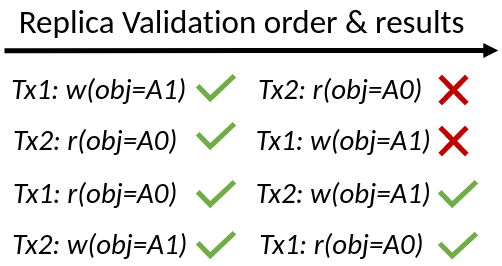
\includegraphics[width= 0.3\textwidth]{./figures/TSO.png}
\end{center}
\caption{TSO validation for a single read/write conflict}
\label{fig:TSO}
\end{figure}
When execution results match the pre-defined timestamp order, no aborts are necessary. Our challenge then becomes to 1) assign appropriate timestamps and 2) coordinate execution in a way that maximizes such coherence; the presence of byzantine participants (clients/replicas) complicates this.

1) First, we require a timestamping service that (accurately) reflects the real-time execution start. While we assume that clocks are loosely synchronized across honest participants, byzantine participants may diverge arbitrarily in undesirable fashion. Read transactions with timestamps that are too far in the future can cause all successive "younger" transactions to abort. 
A straightforward way to bound legal timestamps is to rely on a verifiable timestamping phase: A client may query a Quorum of $\geq 2f+1$ replicas for their local time and choose the median which provably bounds byzantine timestamp divergence. This however, entails an extra WAN Roundtrip, increases observed clock divergence due to different replica latencies and requires attaching a Quorum of signatures. To side-step this additional overhead we compromise by allowing clients to optimistically select their own timestamp, but rejecting timestamps above some Threshold. We point out, that both choosing a timestamp that is too small or too large increases the risk of ones own transaction being ignored, thus incentivising clients to select real-time timestamps. In order to facilitate a total serialization order across all clients, we define Timestamps to be tuples of the form $(Time, CID)$. A byzantine client however, may choose identical timestamps for two different transactions. Such ties can be broken by TxID order. Furthermore, this is an observable misbehavior: A replica can safely dency processing from the second transaction received and report the issuing client.

2) Second, in order to maximize coherence between execution and timestamp we desire to minimize both execution and commit (validation \& writeback) time. The smaller the window for out-of-order interleavings, the higher the rate to commit. As previously alluded to, writes are buffered locally, while reads may require WAN roundtrips to provide integrity. This increases the window for conflicting writes to arrive, thus causing read transactions to abort.
Moreover, achieving replication (Validation/Writeback phase) requires additional roundtrips in order to maintain consistency. Consequently, write transactions become committed only after a long time, resulting in successive concurrent reads arriving out-of-order.
To mititage the frequency of read aborts we add three mechanisms on top of TSO, resulting in and implementation of MVTSO (Multiversion TSO):
\begin{itemize}
\item Multiversioning: We store multiple past write versions and allow read operations to "read in the past". This avoids unecessary aborts when read transactions execute only \textit{after} a write with higher timestamp. Previously, long executing read transactions (i.e. multiple sequential reads) could have suffered from a) reading from inconsistent database snapshots due to concurrent writes and b) from their timestamp growing smaller and smaller relative to concurrent write transactions validating at the same times. \fs{fix these last sentences}
\item Read Uncommitted: We allow read operations to optimistically read locally validated, but not fully committed transactions. By making writes \textit{visible earlier}, unecessary aborts for reads that would have previously missed the newer write are avoided.
\item Read Timestamps: We allow read operations to claim \textit{Read Timestamps} by signaling replicas to abort out-of-order writes (writes with smaller timestamps). This fairness policy implements a bias towards read operations, by aborting writes instead of reads. Since most workloads are read dominated and write-only transactions can re-execute more swiftly, this is an intuitively sensible trade-off. In section Y (Retries) 	we discuss an optional modification to support read-modify-write transactions. \fs{retries}
\end{itemize}


Note, that for write heavy workloads, or workloads without read/write conflicts MVTSO degenerates to TSO.

Algorithm \ref{mvtso} shows the necessary validation check to preserve Byzantine-Serializability. 
Given a transaction TX finalized execution state, i.e. its read-set, write-set and dependencies, and a proposed timestamp, the validation check returns \textit{Abstain/Abort} (we discuss the distinction further in section X (validation)) if a conflict has been detected. Otherwise, a replica tentatively \textit{Prepares} a transaction by adding its reads and writes to the $PreparedDB$, making its writes visible and evaluating future transactions against it for conflicts. Regardless of the outcome, a replica garbage collects all Read Timestmaps (RTS) associated with the transactions reads (indexable by matching TS).
It then waits for necessary dependencies (uncommited writes that were read) to be resolved. \fs{(ADD note: dependency blocking only needs to happen at the shard where the dep came from)} \fs{should unprepare if dep aborts; this avoids more dependencies to be formed unecessarily}
If all dependencies resolve do so successfully the check returns Commit, and otherwise un-prepares the transaction and returns Abstain/Abort. We remark, that the concurrency control check is serialized and executed atomically for each transaction.


 
%%%%%%%%



\fs{cannot move prepare after its own dependencies are resolved, otherwise other transactions could have prepared in the meantime which would not be legal. CC check needs to be atomic, i.e. have locks for all relevant keys and be serialized.  If dep depth max 1, one could technically move the dep wait to the front; but this diminishes the chances for the transactions commit when waiting a long time for deps to be resolved first which is undesirable.}
\fs{cannot return abstain for a TX whose readset is not in the local Database: other replicas might have seen the required writes. (And for byzantine clients we dont care if they fake their reads). need to be able to decide just on local knowledge}


\begin{algorithm}
\caption{MVTSO-Check(TX, TS)}\label{mvtso}
\begin{algorithmic}[1]
\If{\textit{$TS > localClock + \delta$}} %  || $TS < lowWM$ || $\exists d \in dep: d.TS < lowWM$} } dont mention garbage collection part here, it only confuses
\State \Return ABSTAIN
\EndIf


%Should be PreparedDB and DB for lookups: Check: exists read with TS and version. I.e.: Exists (TS) in DB[key][writes] and (TS, rv) in DB[key][reads]
\For{\textit{$\forall key,version \in \textit{TX.read-set}$}}
        \If{$ \exists TX2 \in CommitLog: key \in \textit{TX2.write-set} \land version < \textit{TX2.TS} < TS$}  
          \State  \Return ABORT, \textit{TX2, TX2.CommitCert}
        \EndIf
         \If{$ \exists TX2 \in Prepared: key \in \textit{TX2.write-set} \land version < \textit{TX2.TS} < TS$}   
          \State  \Return ABSTAIN, \textit{TX2}
        \EndIf
          
   %     \If{$ \textit{dep[key]} == null \land version \notin prepared-reads[key] \cup  CommitLog \cup AbortLog $}   
    %      \State  \Return $\textit{Proof-of-Misbehavior}$
    %    \EndIf
		   
        
        
\EndFor

\For{\textit{$\forall key \in \textit{TX.write-set}$}}
        \If{$\exists TX2 \in Prepared/CommitLog : \textit{TX2.read-set[key].version} < TS < TX2.TS$} % \land TX \notin TX2.dep  ..Not necessary: if the read depends on our write for this key then it is implied that the version is not smaller.
          \State  \Return ABSTAIN, \textit{TX2} || ABORT, \textit{TX2, TX2.CommitCert}
          %\State  \Return RETRY, %$\textit{TS_{new} | \forall TS_{new} > TX2.TS}$ // 
        \EndIf
        \If{$\exists RTS \in key.RTS: RTS > TS \land TX \notin RTS.dep$} %Here you do not know about the version, so you must include the exception on the dep
          %\State  \Return RETRY, %$\textit{TS_{new} | \forall TS_{new} > TX2.TS}$ // 
          \State  \Return ABSTAIN
        \EndIf

\EndFor
\State Prepared.add(TX) 


\While{$\exists d \in dep: d \notin CommitLog \cup AbortLog $)}
\State Wait
\EndWhile

%structure it in a way that is better
\For{\textit{$\forall d \in dep$}}
		\If{$ d \in AbortLog $}
			Prepare.remove(TX)
			\State \Return ABORT, d.AbortCert
		\EndIf
		
		%%%%%%%%%%%%Only relevant to retries
        %\If{$ d \in CommitLog $}
        %	\If{$d.TS > TS$}
        %	\State \Return ABORT, d.CommitCert  %% Remove because it is only a Retry optimization
        %  	\EndIf
       
		%\Else 
		%\State \Return ABORT, d.AbortCert
		%\EndIf
\EndFor


\State \Return COMMIT


\end{algorithmic}

\end{algorithm}

\paragraph{Replica State}
\fs{Need to modify MVTSO pseudocode to match the replica strucutres? or is the way it is expressed rn better.}
In order to perform the MVTSO-check (efficiently), a replica maintains several data strucutres as seen in Figure \ref{fig:RS}): It keeps track of its \textit{Database}, of \textit{Ongoing} transactions, and \textit{Completed} transactions. The Database is manifested as multi-versioned key value store. It contains both the writes and reads of all committed transactions.
Further, completed transactions are logged in respective Commit and Abort Logs, that effectively represent the ledger of all processed transactions. Since replicas process transactions out of order, we store this log as a set. This allows us to perform swift lookups for dependencies as transactions can be identified by their TxID. 
Replicas keep track of ongoing transactions and their respective validation protocol state (see section Y). Additionally, it maintains a temporary key-value store $PreparedDB$ of tentatively committing (prepared) transactions to service both optimistic reads and check for conflicts. 
When a transaction performs the MVTSO-check, its dependencies may not yet be present in either Commit or Abort logs. To avoid busy waiting, a replica temporarily suspends the MVTSO-check for the current transaction until all dependencies are resolved, allowing it to process other transactions pending validation. To facilitate this, a replica keeps track of two additional datastrucutres, \textit{Dependents} and \textit{WaitingDeps}. Dependents maps a transaction to all its known dependents, i.e. for a transaction TX1 with dependencies \{TX2, TX3\} Dependents contains two entries (TX2: \{TX1\}) and (TX3: \{TX1\}). Vice versa, WaitingDeps, contains all unresolved dependencies for a given transaction, i.e. (TX1: \{TX2, TX3\} in the given example. When a transaction (e.g. TX2 completes) a replica can search Dependents to find all of its dependents, and update the dependents WaitingDeps set accordingly. A replica may then resume a suspended MVTSO-check for transaction TX by either Abstaining/Aborting if a dependency was added to the AbortLog, or returning Commit if $Deps[TX]$ is empty.
In section X (Writeback) and Y (Garbage Collection) we discuss how to garbage collect ongoing transaction state and completed transaction state respectively. 




\begin{theorem}
The set of transactions for which the MVTSO-Check returns Commit is Byzantine-Serializable. 
\end{theorem}
\begin{proof}
We first show, that the MVTSO-Check never returns Commit for two conflicting transactions TX1 and TX2.
WLOG, assume that TX1 is validated before TX2 and MVTSO-Check(TX1, TX1.TS) returns Commit. This implies that all reads and writes of TX1 are \textit{Prepared}, (i.e. in PreparedDB).
We show by case distinction that TX2's validation cannot return Commit:
\begin{itemize}

\item \textbf{TX1.TS < TX2.TS} By timestamp order, the excution results of TX1 and TX2 should be equivalent to a serial schedule in which TX1 happened \textit{before} TX2. A conflict only arises, if TX2 performed a read that should have seen TX1's write, i.e. if TX2's $read.version < TX1.TS$. By lines 3-7 TX2 must Abstain/Abort since TX1 $\in Prepared$. 

\item \textbf{TX1.TS > TX2.TS:} By timestamp order, the excution results of TX1 and TX2 should be equivalent to a serial schedule in which TX1 happened \textit{after} TX2. A conflict only arises, if TX2 attempts to write a version that TX1 should have observed, i.e. if TX1's $read.version < TX2.TS$. By lines 8-10 TX2 must Abstain/Abort since TX1 $\in Prepared$. 
\end{itemize}

We now show, that every honest clients transaction is \textit{legal}, i.e. its reads are based on committed writes. This follow straightforward from Execution protocol: An honest client only reads values that are either committed, or optimistically reads by claiming a dependency on uncommitted writes. By lines 14-18, a TX with dependencies only Commits if all of its dependencies Commit, implying that it read committed writes.

Consequently, all honest clients experience Serializability, and thus, the MVTSO-check maintains Byzantine-Serializability.
\end{proof}

\textit{Aside:} Consistent with our definition of Byzantine-Isolation, byzantine clients may issue ficticious Read-Sets comprised of arbitrary read versions and values. However, these have only limited external effect on concurrent writes. We distinguish two extreme cases: 1) $read.version \rightarrow 0$: This case is equivalent to simply reading stale data, and effectively reduces MVTSO to TSO as conlflicts are evaluated only on basis of the transaction timestamps (i.e. Abort write if: write.TS < read.TS). 2) $read.version \rightarrow read.TS$: In this case there are no conflicts as a write is never "missed" by a previous read.

In order to empower \textit{Read Timestamps} we add an additional bias in \ref{mvtso} line 11. Writes that conflict with tentative reads are conservatively Abstained. If there exists a read that did not but should have observed the write ($read.TS > writes.TS$), we conservatively decline the write. We discuss possible read timestamp abuse by byzantine participants, and how to avoid it, in section X (Optional Modification). In Indicus, both execution and validation occur out-of-order across replicas. Thus, it is possible for the read timestamp of a read transaction that depends on another write transaction to arrive at a subset of replicas \textit{before} the write transaction validates. This could cause us to conservatively Abstain the write transaction, causing an unecessary cyclic Abort. To avoid this, clients asynchronously disseminate their dependencies to all replicas as soon as they claim them (see execution step 3). Once received, a replica can grant read timestamp \textit{exception} and admit a write if ($write \in read.dep$) (Alg. \ref{mvtso} line 11). Granting exceptions is not necessary in order to maintain safety; It merely implements an additional layer of protection in order to minimize the window of cyclic aborts, in which a client inadvertently aborts its own transaction. \fs{Should not rely on deps beyond depth 1, because those could be both byz and not claim exceptions and abort themselves always if they set up beforehand}

In the following section we will show how to design a replicated validation scheme that upholds Isolation guarantees and maintains consistency even when replicas validate out-of-order.




%-------------------------------------------------------------------------------
\subsection{Validation}
%-------------------------------------------------------------------------------

The goals of the Validation phase design are threefold: i) It needs to preserve Isolation guarantees between transactions, ii) It should embrace partial ordering \fs{weird}, while minimizing commit latency and  maximizing scalability, and iii) it should be \textit{leaderless}. Satisfying these goals requires ovecoming several challenges. In order to maximize parallelism and embrace partial ordering, Indicus allows replicas to process requests out of order. Consequently, replicas may temporarily be out of sync, and hence return different results. Such divergence must be reconciled in a way that maintains Isolation, but not overly conservatively in order to maximize the ability to commit successfully and bound the impact of byzantine participants. Further, Indicus designates clients as validation coordinator for its own transactions. The respective protocol must tolerate client failures such as crashes, omission/stalling, equivocation, or replays and allow for consistent recovery. 

The Validation protocol can be broken down into two functionalities: Voting and Logging.
Since Indicus aims to prescribe a partial order, Replicas need to agree on results, rather than an Ordering. To do so in a leaderless fashion, they vote. As in any democratic decision, these votes are then aggregated into a decision. In the case of Indicus, the client acts as the transaction coordinator who aggregates and relays results (along with necessary evidence).
 In order to maintain consistency in the presence of failures (i.e. no two honest replicas finalize different Commit/Abort decisions), this decision must be logged prior to returning, guaranteeing that a replay of any Writeback is idempotent. \fs{This two step decision protocol resembles Two-Phase Commit.} However, since we cannot trust a byzantine coordinator to persist a decision, nor could we retain liveness during a crash, we delegate the decision logging to the replicas.
 
 \fs{any traditional SMR replication protocol could be used to do Logging. However it would be vastly unecessary as ALL requests are independent at this point, so an order is in fact completely obsolete. Our solution looks basically like Q/U, because unordered broadcast/acknowledgement suffices. Byzantine clients equivocating maps to client "contention" in Q/U. Q/U is not live when that happens however; we build additional fallback view change mechanism.}

The voting phase requires a single round-trip to all replicas, whereas the logging phase requires at most one round-trip \fs{in Indicus5 and at most two round-trips in Indicus3.}. When execution is \textit{gracious} Transactions can be committed on the \textit{Fast-Path} in a single-round trip as an explicit logging round is not necessary. Figure \ref{fig:ValO} gives an overview of the protocol.

\begin{figure}

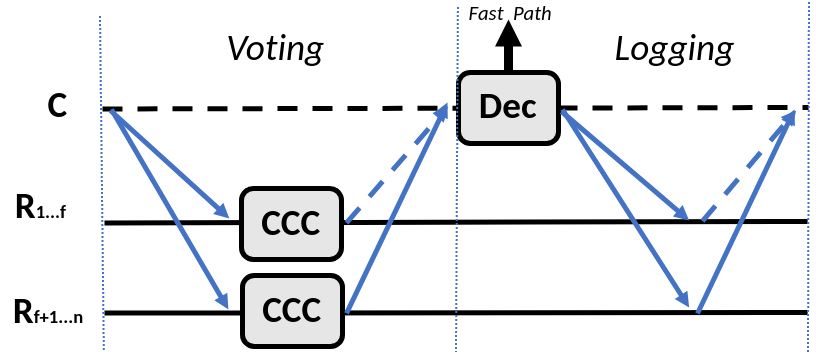
\includegraphics[width= 0.4\textwidth]{./figures/Validation.png}

\caption{Validation Protocol}
\label{fig:ValO}
\end{figure}

\begin{figure}[t]
  \begin{mdframed}[roundcorner=10pt]
 	\textbf{TX Val State}
 	\begin{itemize}
 	\item TxID
 	\item originalClientID
 	\item interestedClients = \{CID\}
 	\item ClientSeqNo
 	\item Transaction = TXExecState
 	\item vote   ~~~~~~~~~~//Prepare1R
 	\item decision = (dec, view.no) ~~~~~~~//Prepare2R
 	\item optional: dec proof = \{$votes_r$ \} ~~~ //Only for Retries and Indicus3
 	\item current.view
 	\end{itemize}
  \end{mdframed}
  \caption{Transaction Validation State at Replicas}
  \label{fig:Val}
\end{figure}

To describe how the protocol operates in detail we follow a single-shard transaction through the system. Figure \ref{fig:Val} shows the protocol state replicas maintain for each ongoing transaction.

\fbox{\begin{minipage}{21em}
\textbf{(1: C $\rightarrow$ R)}: Client sends Prepare request to all Replicas within the Shard.
\end{minipage}}

Upon deciding to Commit in the Execution phase, a Client initiates Validation by sending a message $Phase1 \coloneqq \langle Prepare, TxID, TX \rangle_{\sigma_c}$ to all Replicas.

\underline{Additional subtlelties}: A client may not equivocate this request. Any change to the TX state changes the TXiD and hence is treated as seperate TX. 

\fbox{\begin{minipage}{21em}
\textbf{(2: R $\rightarrow$ C)}: Replica receives validation request, processes it and returns vote to Client.
\end{minipage}}
A replica validates Timestamp and Dependency integrity of the request. It then evaluates Read and Write Sets for Isolation conflicts using the MVTSO Concurrency Control Check (CCC), as shown in algorithm 1. The concurrency check is entirely based on local knowledge of previously committed, and concurrently ongoing transactions. If successful, a replica updates its set of potenially committable transactions (Prepared) and returns a Commit Vote to the client. If unsuccessful, a replica returns an Abort/Abstain Vote to the client, along with evidence justifying the decision. It sends a message $Phase1R \coloneqq \langle TxID, vote \rangle_r$.



\underline{Additional subtlelties}: A replica validates whether all read versions are legal, i.e. whether the $version < TS$, and whether all entries in the dependency set are legal, i.e. whether f+1 matching signatures exist. If this is not the case, a replica rejects the request and submits a Proof of Misbheavior (PoM) to expel the client from the system. A byzantine client may neither match read set and dependency set, nor match read set to the involved shards. This is tolerated, as a byzantine client chooses whether to experience Isolation and Atomicity. Illegal reads, or un-committed writes do not have external effect, but are auditable in the committed ledger to trace misbehavior. \fs{can just make it a PoM too and ignore, probably simpler and for the better}
\fs{ In effect, any claimed deps implies a client did those reads, but he does not necessarily have to include them} 
A replica updates its $OngoingTX$ set by adding a pair $(TxID, state)$, where $state$ is an object containing relevant protocol metadata, such as the Client Phase1 request or the MVTSO Check decision (to service replays and avoid re-execution). Importantly, a replica never changes its Voting decision, because re-execution could leave to different results. In section X we discuss an optimization to allow this behavior. If voting Abort, a replica additionally returns the transaction causing the conflict and a respective CommitCertificate to prove that transactions finality. If voting Abstain, a replica instead returns the signed Phase1 request of the conflicting Transaction. \fs{For the best "progress" guarantee a replica would need to return ALL conflicting TX, in order to allow a client to finish all of them. However, this a) often needlessly costly (check cannot stop on first conflict + sending more message content), and b) does not guarantee that there will be no new conflicts by the time the TX tries again.} \fs{if we dont want to allow to commit a conflicting TX, then they could just reply with the TxID, and the TxID could be used to vote default abstain once the timeout has expired.}
Lastly, a replica starts a timer to monitor the clients progress.
%%%%%%%%%%%%%
Access control is beyond the scope of this work, but a replica would additionally check for all writes whether access control exists and reject the transaction otherwise.


\fbox{\begin{minipage}{21em}
\textbf{(3: C)}: Client waits for vote replies.
\end{minipage}}
A client waits for at least $n-f$ ($4f+1$ in Indicus5) distinct replica votes, or more, up to a system specified timeout. 

\fbox{\begin{minipage}{21em}
\textbf{(3a: C)}: Client receives Threshold of matching votes and returns to application. Proceeds to Writeback
\end{minipage}}
In any of the following 3 cases, a client may short-circuit waiting for additional votes and omit a dedicated Logging round:
\begin{enumerate}
\item \textbf{$1$ Abort vote w/ Conflicting TX \& CommitCertificate}: The client validates the integrity of the CommitCertificate (CC) and returns the shard decision $(TxID, Abort, \langle ConflTX \rangle_{CC})$.  \fs{clients (and replicas during writeback) must validate the legitimacy of the conflict against the certified Transaction - it might be simpler for exposition to not include this case and just always vote abstain - this can be called Abort too then.}
\item \textbf{$3f+1$ Abstain votes w/ Conflicting TX}: The client returns the shard decision $(TxID, Abort, \{\langle AbstainVote\rangle_r\})$. 
\underline{Additional subtlelties}: The client temporarily stores the conflicting TX Phase1 requests, in order to be able to drive that transactions termination if necessary/desired (see Section X - Granting Liveness).
\item \textbf{$5f+1$ Commit votes}: The client returns the shard decision $(TxID, Commit, \{\langle CommitVote \rangle_r\}$
\end{enumerate}
Any of such Quorums forms a \textit{Shard-Certificate} and proves the decision. A client uses this Certificate to return to its application and issue the Writeback.
\fs{need to distinguish with Indicus3: can still abort FP, but not commit.}

\fbox{\begin{minipage}{21em}
\textbf{(3b: C $\rightarrow$ R)}: Client receives inconsistent results and suggests a consistent decision to Replicas for Logging
\end{minipage}}
If a client does not receive the necessary thresholds of votes to return, it must continue on the \textit{Slow-Path}. To do so, it aggregates the votes according to a conservative \fs{not really} decison rule:
If there exists a $CommitQuorum \coloneqq \frac{n+f+1}{2}$ ($3f+1$/$2f+1$ in Indicus5 and Indicus3 respectively) of Commit Votes, the Slow-Path decision is Commit, otherwise it is Abort.
A client broadcasts a message $Phase2 \coloneqq (TxID, decision, \{\langle votes \rangle_r\}$.

\underline{Additional subtlelties}: A client forwards a Quorum of $\geq n-f$ votes to the replicas. This is necessary to prove the Slow-Path decision is consistent with Isolation guarantees. Effectively, replicas make the decision for themselves. Note, that a byzantine client may equivocate the decision by relaying different Quorums.

\fbox{\begin{minipage}{21em}
\textbf{(4: R $\rightarrow$ C)}: Replicas receive, validate and echo decision
\end{minipage}}
A replica confirms that the Decision matches the Quorum, by evaluating the decision rule itself. It then returns the decision to the client by sending $Phase2R \coloneqq \langle TxID, decision \rangle_r$. \fs{with retries this needs to include the timestamp}

\fs{Note: One could think that it could be ok for replicas to un-prepare transactions that have the decision abort. This would be a tempting optimization because it avoids conflicts as early as possible. However, this would not be safe: Consider an example in which 4 out of 6  prepared and voted commit and one of them was byzantine. The client could use a Quorum including 2 abstain votes to decide Abort and send it to a single correct replica that already prepared. Then there may only be 2 replicas out of 6 that have it prepared and a conflicting TX could be committed. But the orginial TX could also be committed, since only 5 commit acknowledgements are necessary. }

\fbox{\begin{minipage}{21em}
\textbf{(5: C)}: Client returns shard-decision to application and proceeds to Writeback
\end{minipage}}
A client waits for a Quorum of $n-f$ matching Phase2 Replies. Such a Quorum forms a \textit{Shard-Certificate} and proves the decision. A client uses this Certificate to return to its application and issue the Writeback.

\underline{Additional subtlelties}: If a client equivocated, it will never receive a Shard-Certificate. An honest client however, is guaranteed to receive matching Phase2 replies. 

%%%Optional for Indicus3
\iffalse
\fbox{\begin{minipage}{21em}
\textbf{(5a: C)}: Client returns Commit to application
\end{minipage}}

\fbox{\begin{minipage}{21em}
\textbf{(5b: C $\rightarrow$ R)}: Client sends consistent echo to Replicas
\end{minipage}}

\fbox{\begin{minipage}{21em}
\textbf{(6 : R $\rightarrow$ C)}: Replicas echo 
\end{minipage}}
\fi

\fs{should perhaps come after Writeback (which is brief) in order to frame the proofs. But then we need to show Atomicity also. Durability. Conistency. }
We now briefly allude to the correctness of respective decision rules and Quorum sizes.



We consider a decision (Commit, Abort) to be \textit{logged} when it is possible for some Shard-Certificate to exist, i.e. as soon as the necessary certificate Quorums exists at some Replicas.
Figure \ref{fig:FigureSP} summarizes the relevant nomenclature.

\begin{figure}
\begin{center}
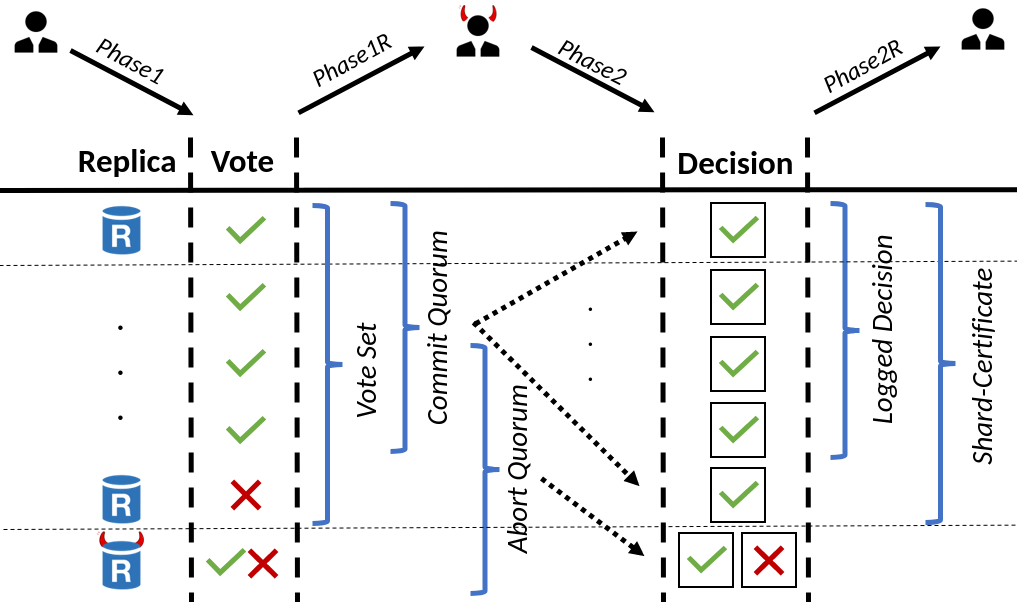
\includegraphics[width= 0.5\textwidth]{./figures/Nom2.png}
\end{center}
\caption{Validation Nomenclature, Slow-Path. Note, that a byzantine client may equivocate Phase2 decisions by including Commit and Abort Quorums respectively. Byantine replicas may store multiple votes and decisions.}
\label{fig:FigureSP}
\end{figure}

\subsubsection{Correctness}
We show, that a \textit{logged} decision is final:
\begin{theorem}[Saf]
A logged decision is durable, and there can ever exist \textbf{at most one} logged decision.
\end{theorem}
\begin{proof}
We show this by case distinction. Slow-Path: A Slow-Path decision is \textit{logged} if $\frac{n+f+1}{2} = 3f+1$ ($LoggedQuorum$) honest replicas have adopted the decision, since $n-f = 4f+1$ votes suffice to form a Shard-Certificate and $f$ byzantine participants may decide arbitrarily. Thus it is impossible for two logged decisions to co-exist, as any two $LoggedQuorums$ must intersect in $f+1$ honest replicas that will only ever accept one decision - a contradiction. Furthermore, honest replicas do not change their decision, and hence a slow-path logged decision persists. Fast-Path: We distinguish three sub-cases. The existance of $4f+1$ Phase1 honest commit votes, implies that any Slow-Path decision must result in a commit decision, since any Quorum ($n-f = 4f+1$) is bound to include $3f+1$ commit votes. Vice versa, the existance of $3f+1$ honest Phase1 abstain votes, implies the impossibility of any Slow-Path commit decision. Moreover, both the above cases mutually exclude each other. Lastly, 1 valid Abort vote implies the existance of a logged decision for the conflicting Transaction. By Induction \fs{that TXs logged decision never changes}, and Quorum intersection, this implies that at least $3f+1$ honest replicas will vote to Abstain the ongoing transaction and hence it is impossible to ever log a commit decision for the ongoing Transaction.
\end{proof} 

Note, that since replicas never change their decision, it is possible for there to never be any logged decision if a byzantine client equivocated its Slow-Path Quorums. In order to reconcile this, we design and discuss a recovery mechanism in section X which relaxes the requirement on persisting a decision.  


\begin{theorem} 
Indicus maintains \textit{Byzantine-Serializability}.
\end{theorem}
To prove that this is the case, we show that for any two conflicting transactions, at most one can be committed.
\begin{proof}
Let TX1 be a transaction with logged decision Commit \fs{, i.e. TX1 has either already committed at or is bound to commit at all honest replicas}. Let TX2 be a conflicting transaction, that if committed, would violate Byzantine-Serializability. Assume TX2 too, managed to log a commit decision. By the protocol (and proof of Theorem Y -the above theorem), at least  $\frac{n+f+1}{2} = 3f+1$ commit votes are required to log a decision, and no honest replica changes its vote. By Quorum intersection, at least one honest replica must have voted commit for both TX1 and TX2. WLOG, this replica received TX1 before TX2, and, by the correctness of the MVTSO-check \fs{Theorem in CC section}, must have voted Abort or Abstain for TX2. A contradiction.
\end{proof}




\begin{theorem} 
Indicus maintains Byzantine Independence in the absence of network adversary.
\end{theorem}

We show, that once a Client submits a transaction for validation, the result cannot be unilaterally decided by any byzantine participant, be it client or replica.
\begin{proof}
First, we observe that a client may never choose a result itself, but only implicitly influence a decision by choice of Slow-Path Quorum. Specifically, a byzantine client cannot single-handedly decide to abort its own transaction and consequently, cannot single-handedly force potentially dependent transactions to abort as well. \fs{this is not quite true, need to expand on it}
Second, any Quorum decision requires at least one honest replicas vote. In particular, a $f$ byzantine replicas may vote to abstain arbitrarily (by always reactively generating a ficticious transaction), but at least one additional honest abort vote is necessary to result in an abort (at least $f+1$ additional honest votes if the network is synchronous with regards to the timeout $\delta$). 
Thus, in order to artificially cause transactions to abort, a conflicting transaction must be generated (artificial congestion). However, to do so strategically and reliably \fs{deterministically}, the adversary must control the network in order to guarantee the artifical transactions arrival at honest replicas \textit{before} the original transaction. 

\fs{likewise 2 byz clients may not abort each other:Consider as a more subtle case the scenario in which two colluding byzantine clients attempt to abort each other by sending 2 tx that either conflict (or the one depends on the other) to different subsets of replicas in different order. In order to do so they need to control the network. If they DO manage to set this up, they could abort any transaction that ends up depending on either of them. However to do so deterministically, they need to set up accordingly BEFORE the honest TX arrives (which requires network control) and KNOW the keys to do so strategically (which we assume they dont: see properties section assumption);  1 byz client could issue two tx that arrive only in fifo order so its fine too (more than some threshold t of concurrent tx will be counted as PoM)}
Thus, when the network is not adversarial, validation decisions are \textit{Byzantine Independent}.

\fs{need to add the case of dependency trying to get aborted by its own dependent. this too is up to the network: A byz replica does not know that there is a dependent until the exceptions or prepares are being issued. needs to have faster connection in order to still abort. if there are multiple levels then the colluders could already pre-abort each other: example: out of order at 3 replicas each. any TX coming after that claims a dep is doomed. But this is not deterministic: it requires preemtive setup, but keys are not known}
\end{proof}
We note, that Indicus3 does not have this property: Byzantine Clients can always abort themselves, which is undesirable when wanting to allow dependencies. \fs{re-iterated in Indicus3 section - can be cut here}



 
 \iffalse
%-------------------------------------------------------------------------------
\subsection{Consistent logging.}
%-------------------------------------------------------------------------------
\begin{figure}
\begin{center}
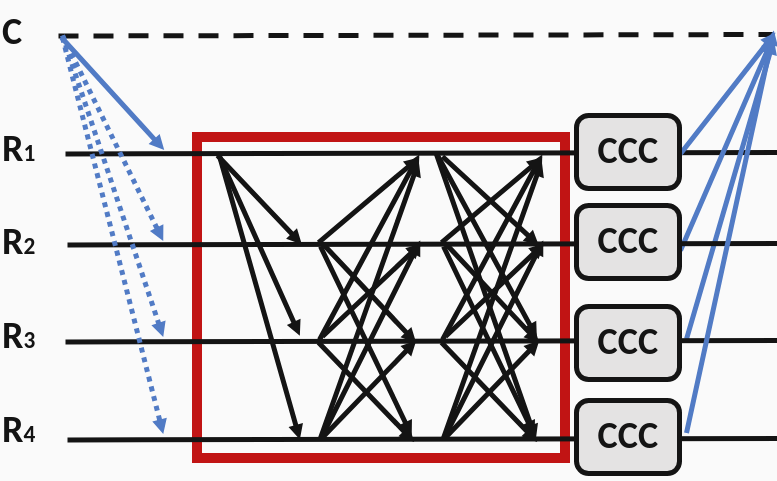
\includegraphics[width= 0.4\textwidth]{./figures/AB.png}
\end{center}
\caption{Atomic Broadcast}
\label{fig:Figure1}
\end{figure}


\begin{figure}
\begin{center}
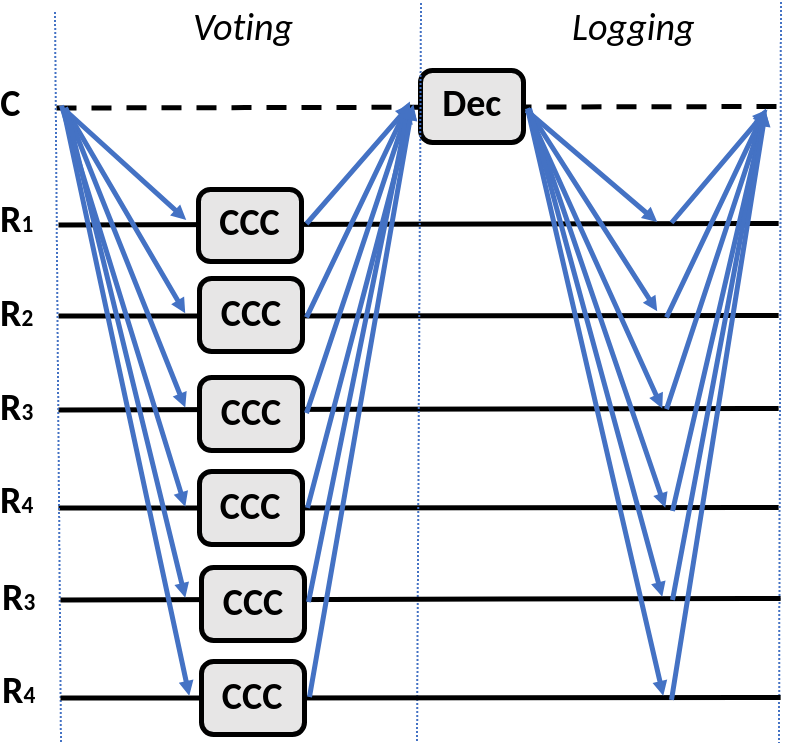
\includegraphics[width= 0.4\textwidth]{./figures/5f+1.png}
\end{center}
\caption{Logging}
\label{fig:Figure1}
\end{figure}

Principles and challenges

protocol overview: pic
\fi

%-------------------------------------------------------------------------------
\subsection{Writeback and Multi-shard 2pc}
%-------------------------------------------------------------------------------

Validation occurs on every Shard that a transaction spans. The goal of the Writeback phase is to aggregate all relevant shard-decisions and to inform replicas of finalized Commit or Abort decisions. This is necessary in order for replicas to be able to garbage collect meta-data of ongoing transactions, and to allow consecutive transactions to reliably observe the updated state. Any finalized decision must respect all shard-decisions relevant to a transaction. Thus, all decisions are aggregated according to standard two-phase commit. Only if all shards agree that a transaction may commit (i.e. there exist commit certificates for every shard), then a transaction may commit. The protocol is simple:

\textbf{1. A coordinator waits for all shard decisions, including certificates}\\
\textbf{2. The coordinator broadcasts a $Writeback \coloneqq (TX, decision, \{certificates_S \} )$ message to all replicas in all relevant shards}.\\

\fbox{
\begin{minipage}{21em}
\textbf{(1 : Coord $\rightarrow$ S)}: A coordinator aggregates decisions and forwards them to all relevant shards.
\end{minipage}
}

A coordinator waits for all shard decisions, including certificates. The coordinator aggregates the decisions and broadcasts a $Writeback \coloneqq (TX, decision, \{certificates_S \} )$ message to all replicas in all relevant shards.
\underline{Additional subtlelties:} A transaction includes a set \textit{InvolvedShards} of relevant shards . A \textit{Writeback} message is only valid if there exists a shard-certificate for every involved shard. The Writeback message does not need to be signed. A single Abort certificate may short-circuit the coordinator wait as it suffices to Abort.\\





\fbox{\begin{minipage}{21em}
\textbf{(2 :  S)}: Replicas in a shard validate and finalize the writeback decision.
\end{minipage}}
Upon reception of a \textit{Writeback} messgage, a replica validates whether its own shard is involved, and if so whether a) there exist a single Abort shard-certificate, or b) Commit shard-certificates for all involved shards. If not, a replica rejects the request. If the request is valid a replica does the following:\\

\textbf{Abort:} A replica removes the transaction from its OngoingTX set and PreparedDB, and adds the transaction, along with the shard-certificates to its AbortLog. Furthermore, if a set of dependents existed in the Dependents set, the replica resumes the blocked MVTSO checks for the dependents and votes Abort. It clears the WaitingDeps set and all corresponding WaitingDeps[dependent] entries in the WaitingDeps set.
\fs{this abort log somehow needs to be able to be garbage collected. abort certs are necessary to prove a dependency abort is legitimate - could be replaced by voting abstain}\\


\textbf{Commit:}
Analogous to Abort, a replica updates OngoingTX set and Prepared DB, but adds the transaction, along with certficates to the CommitLog. It additionally updates the key-value Database by creating entries for each read and write. \fs{optional notifiy for early abort:} Furthermore, for all write keys, it removes all existing Read Timestamps (RTS) that are smaller than the committed TXs Timestamp and notifies the clients that issued them. \fs{this allows those clients to abort and restart execution early - requires the commit proof to be accepted by clients}. 
Lastly, if a set of dependents existed in the WaitingDeps set, the replica updates the respective dependencies set for all dependents in Deps (i.e. $Deps[dependent] \setminus TX$). If for any dependent $Deps[dependent] = \emptyset$ then the replica resumes the blocked MVTSO check for the dependent.



\underline{Additional subtlelties:}
\fs{Cut this if we go back to normal Atomicity def. In this case: The involved shards need to match the read/write sets. This requires replicas to know which keys exist in the DB. This is necessary anyways to maintain Invariants across shards} A byzantine clients transaction might include reads and writes for a shard, yet not include the shard in the \textit{InvolvedShards} set. This is consistent with the definition of Byzantine-Atomicity. Moreover, a replica would have never processed a Prepare message if InvolvedShards does not include its ownShard, and hence no garbage collection is necessary.\\

We point out, that the Writeback coordinator need not be the client issuing the transaction, but can in fact be an arbitrary party (client or replica) that is interested in completing the Writeback. This follows straightforwardly from Theorem Y: Any certified shard-decision implies the existence of a logged decision, and hence the Writeback phase is idempotent.
We utilize this to drive the recovery protocol outlined next. 



%-------------------------------------------------------------------------------
\subsection{Granting Liveness}
%-------------------------------------------------------------------------------
\fs{This needs to come out more clearly: shard decision implies logged decision, but there may not be any shard decision. We want logged decision to imply that any honest client can generate a shard-decision. There may neither exist a logged decision, nor enough replicas voting for a shard-decision.
}
Indicus operates under the premise that clients experience progress indepentently. Since agreement occurs on a per Transaction basis (each client drives its own validation) and replicas may process requests out of order, there exists no shared notion of system progress. When all participants are honest progress is trivially guaranteed for every client. Byzantine clients however, may bring execution, validation or writeback to a halt for their own transactions. For example, a byzantine client may either stall during all phases, or equivocate during validation logging. The latter case lets replicas diverge on the decision value (Commit/Abort), making impossible to arrive at a shard-decision, and hence degenerates to a form of stalling too. When all transactions are commutative this phenomenon requires no action: Any client \textit{chooses} whether to adhere to the protocol and experience progress, or not. However, when this is not the case, and transactions depend on each other, either explicitly (through reading anothers transactions uncommitted write), or implicitly (through read-write conflicts), liveness is no longer independent. For instance, a claimed dependency might be of byzantine origin (explicit dependency) and never terminate, causing the dependent to stall helplessly itself. Alternatively, an uncommited write, yet unclaimed dependency, (implicit dependency) might forever cause all consecutive read transactions to abort  \fs{since we only return the max uncommitted as prepare it might not be possible to get enough matching..}.
Thus, in order to allow clients to intertwine their fate with concurrent transactions, we must strengthen Theorem X. We define Liv:

\begin{theorem}[Liv] \fs{change to: there should exist a shard-decision?}
For any transaction, there exists \textbf{exactly one} logged decision, if desired by an honest client.
\fs{Any request that an honest client is interested in (broader than just "issued by an honest client") eventually completes}
\end{theorem}
Intuitively, this property allows honest clients to experience progress, if they desire to. To achieve this, we must relax the requirement that replicas may never their decision, while preserving Theorem X (rename to Safety).


A naive solution would be to allow any client to drive another clients protocol. This is problematic, since \textit{interested} clients could concurrently make inconsistent decisions and consequently never make progress \fs{an all to all between replicas has the same behavior as multiple clients potentially, need single leader to guarantee that all agree on Quorum}. Electing a single client is similarily not live, as there is an unbounded number of byzantine clients that will constructively aid in reconciliation. We circumvent this, by letting concurrent clients replay the protcol, but partially delegating responsibility to the replicas. Concretely, we design a mechanism to elect \fs{endorse ;)} a dedicated \textit{Fallback} replica that is responsible for reconciling diverged replica decisions. Since the number of faulty replicas is bounded, at most $f+1$ leader elections are necessary to make progress when the network is synchronous. A challenge in doing so is to guarantee a live round-robin election. We remark, that in an asynchronous network, leader election might not be possible. This is consistent with known impossibility results (FLP) \cite{fischer1985impossibility} for deterministic agreement (randomized exceptions: BenOr, Honeybadger, BEAT). \fs{this is in accordance with FLP, as no non-randomized protocol can reach agreement in an async setting}. \fs{ Contrary to traditional BFT protocols, system progress is a client local property and we strengthen the liveness condition: We can provide liveness only if the system is synchronous and the client is honest}

On a high level, the recovery mechanism operates as follows: \textit{Interested} clients attempt to run the validation protocol themselves. If a client notices or suspects previously present decision divergence, it issues a \textit{Fallback invocation}, i.e. a request to elect a \textit{Fallback} replica to seize control and reconcile decisions. Such recovery protocol is reminiscent of \textit{view-changes} in traditional BFT SMR protocols, but differs in two core aspects: a) While control changes between fallback replicas (leaders), the protocol is still fully client driven (there are no \textit{view-changes} without client invocation) \fs{client does p1, p2, invocation, writeback}, and b) The fallback mechanism impacts only the ongoing transaction, concurrent transactions keep progressing indepentently. Figure \ref{fig:FallB} gives an overview of Fallback mechanism.

\begin{figure}

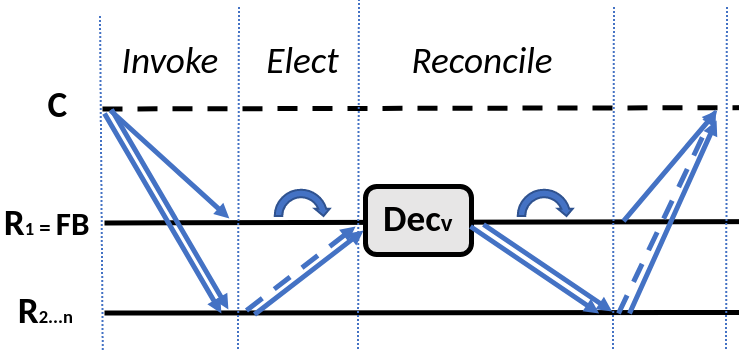
\includegraphics[width= 0.4\textwidth]{./figures/Fallback.png}

\caption{Fallback Invocation}
\label{fig:FallB}
\end{figure}


Below, we detail the protocol by following a transactions life cycle. To start the protocol we assume an \textit{interested} client is in possession of the respective transactions $Prepare$ message, signed by the orignial issuer. \fs{this info can be obtained as part of MVTSO check (f+1 must have the TXID, so an honest replica will have the full TX) for own Tx or through an abort (>f+1 abstains necessary, one honest one will return the conflicting reason - subtlelty: there may be multiple different conflicts but only one is returned; it limits how clients become interested. client learns about full PrepareTX in MVTSO check: returned to it for all TX that have not completed yet. This avoids unecessary info in the exec phase (i.e. reads including full TX)}. For sake of exposition we moreover assume that the transaction has not finalized via Writeback on any replica. We briefly discuss this case afterwards.  




\fbox{\begin{minipage}{21em}
\textbf{(1: C $\rightarrow$ R)}: Client submits backup Prepare request to all Replicas in all relevant shards.
\end{minipage}}
An interested client broadcast a message $Rec-Phase1 \coloneqq (TX.Phase1, CID)$ to all replicas in \textit{InvolvedShards} of the transaction. 

\fbox{\begin{minipage}{21em}
\textbf{(2: R $\rightarrow$ C)}: Replica receives and processes Client request.
\end{minipage}}
If a replica has not previously processed the same Phase1 message, it executes the normal validation protocol and returns the according reply to both the interested client and orignial client. It furthermore starts a time-out on the transaction and adds CID to a list of \textit{InterestedClients} for the respective transaction.
Otherwise, it skips re-execution and does the following: It adds CID to the list of \textit{InterestedClients} and replies with the transactions state stored in $OngoingTX[TxID]$. This state includes the existing $Phase1R$ reply message and, if existing, a decision value ($Phase2R$ message), as well as the \textit{view.no} of the decision. It additionally includes its current $view$.

\underline{Additional subtlelties}: A replica does not need to return $Phase1R$ if it has a decision. The $view.no$ of the original client is zero. Larger views indicate decisions made by a Fallback replica, specifically by the replica with $RID = view.no \% n$. The current view indicates which is the last $Fallback$ replica a client has attempted to elect (Zero, if none yet). Further, a replica delays the timer start until the transaction has no dependencies of its own. This avoids early client evicition and Fallback election in case progress was justifiably inhibited. \fs{re-iterate this to be in sync with mvtso check. Where to block; one could argue the Timestamp is not started because it is still waiting. Hence no replies are issued either.}

%%Fallback start
\fbox{\begin{minipage}{21em}
\textbf{(3: C $\rightarrow$ R)}: Client receives responses and either returns to Writeback or invokes \textit{Fallback} election.
\end{minipage}}

We distinguish the following two cases:

\fbox{\begin{minipage}{21em}
\textbf{(3a: C $\rightarrow$ R)}: A client receives the necessary information to proceed to Writeback.
\end{minipage}}
We consider two subcases:\\
a) If a client receives enough matching $Phase1R$ messages to fulfill a Fast-Path Threshold, it can move on to Writeback. This is safe, because these are logged decisions and imply that any potenially existing Slow-Path decision is the same.
b) Alternatively, if a client receives enough matching (in decision and view) $Phase2R$ messages to form a certificate it proceeds to the Writeback phase.\\


\fbox{\begin{minipage}{21em}
\textbf{(3b: C $\rightarrow$ R)}: A client needs to go Slow-Path or observes inconsistency and requires assistance for resolution.
\end{minipage}}

If a client receives $\geq f+1$ matching decision values and views ($Phase2R$ messages; favors Commit if two matching sets exist) it forwards those to the replicas as proof for a new $Phase2$ message (with the same decision) that it broadcasts to all replicas. If it instead receives $< f+1$ matching decisions it uses the received $Phase1R$ messages to iniate its own $Phase2$ message (identical to validation step, but signed by this client). 
Additionally, if the client received inconsistent decisions (i.e. both Commit and Abort) or $<f+1$ total decision messages that differ from its own proposed decision, it initiates a \textit{Fallback election}. To do so, it broadcasts a message $InvokeFB \coloneqq (TxID, CID, \{view\}_R$. It attaches a set of $4f+1$ signed view messages.  

\fs{refine this}
\underline{Additonal subtlelties}: A client may treat a $Phase2R$ decision as $Phase1R$ vote for the sake of making a new decision. This is safe: If the replica was honest, then this reflects that there existed enough matching votes, and if it was byzantine, it could have voted arbitrarily regardless. \fs{maybe just simpler if replicas include their phase1r as well, but this adds overhead}
 \textbf{View Change Rules:} A client sends a set of signed view messages in order to let potenially diverged replicas now what next view to vote for. However, replicas only adopt a view $v+1$ if the view set includes $3f+1$ \fs{3f+1 should be enough: satisfies that f+1 votes will be found. Can use 4f+1 instead otherwise} votes from view $v$. \textit{Vote subsumtion:} A view $v$ subsumes all prior views: I.e. a replica vote $v$ may count as a vote for all $v' \leq v$. If a byzantine client attempted to diverge the views by only invoking a view change for a subset of replicas, such matching set of views might not exist. 
Replicas that lag behind, may catch up to the maximum view $v$ present $f+1$ times. Such view vote implies, that at least one honest replica has voted for view $v$, and would have done so only, if $2f+1$ honest replicas had previously been in view $v-1$. The possible divergence can be reconciled in a single step, since there must always exist some view $v'$ for which at least $f+1$ honest votes exist in any Quorum (set of 4f+1 voteS) such that $v' \geq max(honest.views) -1 $ (see Vote subsumtion). Thus, the next view change incurs at most 1 additional Roundtrip, since all honest replicas either join max(honest.view) (no additional overhead) or max(honest.view)-1 (another roundtrip to gather $3f+1$ votes.)



\fbox{\begin{minipage}{21em}
\textbf{(4: R $\rightarrow$ C)}:  Replicas receive $Phase2$ messages 
\end{minipage}}
We break the procedure into two components:

\fbox{\begin{minipage}{21em}
\textbf{(4a: R $\rightarrow$ C)}:  Replicas replies with decision
\end{minipage}}
If a replica receives a valid $Phase2$ request (see Validation) it adopts the decision and replies with a corresponding $Phase2R$ message.

\underline{Additional subtlelties:} A replica will buffer requests from $CID \neq originalCID$ and process them only \textbf{after} the timer (set in step 2) expires. If the client request includes a proof of inconsistency (see step 3 and 4b) it will ignore the timer and process the request immediately. If a replica previously adopted a decision, it treats the new request as no-op and returns the stored decision.


\fbox{\begin{minipage}{21em}
\textbf{(4b: R $\rightarrow$ R(FB))}:  Replica additionally receives Fallback invocation and starts election
\end{minipage}}

If a replica receives an $InvokeFB$ message and the original client has timed-out it attempts to elect a new \textit{Fallback replica}. To do so, it follows the \textbf{View Change Rules} and adopts new view $current.view = v$ if $v > current.view$. \fs{effectively when a replica adopts a view, it ignores all older views. Trivial, since it only accepts the first p2 and then never changes. Only thing that changes this is a FB message from higher view.}
Replicas send an $ElectFB \coloneqq (TxID, decision, current.view)_R$ to replica $current.view + TxID \% n$. \fs{this avoids always electing the replicas in the same order - it is both more load balanced and less likely for the initial replica to always be byz.}


\underline{Additional subtlelties:} 
When byzantine clients attempt to invoke elections they may only send the request to a subset of honest replicas, thus never truly enabling an election (requires $4f+1$ elect votes). If there are no concurrent honest interested clients, this can result in replicas being skipped in consideration to become the next Fallback. Moreover, to achieve liveness, we assume a weakly synchronous model, and hence increase the timeouts for each view exponentially.
In order to avoid artificially increased timeouts and enforce a round robin election without skipped candidates, replicas can forward the $ElectFB$ message to all other replicas. If another replica receives $f+1$ such messages, it adopts the view and sends an $ElectFB$ message of its own. This ensures, that for each view, a Fallback is indeed elected (if the network is synchronous within timeout $\delta$). This optimization only aids practical progress in the face of misbehavior and is not necessary for theoretical liveness. To avoid unecessary all-to-all communication, it may only be enforced for views $v > T$, where T is some system defined threshold. \fs{We choose T = f, to avoid false client suspicion in case the first f Fallbacks were byzantine and never replied} 



\fbox{\begin{minipage}{21em}
\textbf{(5: R(FB) $\rightarrow$ R)}:  Fallback aggregates and echos election messages.
\end{minipage}}
The Fallback replica considers itself elected upon receiving a Quorum of $4f+1$ ElectFB messages. It then uses this set of messages to reconcile a decision. It broadcasts a message $FBdec \coloneqq \langle RID, dec, view, \{ElectFB_r\} \rangle_R$, including the new decision and the Elect messages as proof. Effectively, replicas compute the new decision themselves; the Fallback acts as single broadcast channel in order to guarantee that all replicas receive the same Quorum of states.

\underline{Additional subtlelties:} A byzantine Fallback may equivocate Elect Quorums. However, after at most $f+1$ fallback elections a consistent result will be derived (given Synchrony).
\textbf{Decision Reconciliation Rule:} The reconciliation rule is straightforward: $dec_{new} = majority(\{Elect.decision\})$. If a logged decision exists (implies that a shard-decision might exist), any Quorum of $4f+1$ Elect messages is guaranteed to contain $2f+1$ matching decisions (a majority). Vice versa, if $<2f+1$ replicas agree on a decision, then it is impossible for this decision to have been logged. Thus it is guaranteed that logged decisions persists and otherwise an arbitrary decision qualifies since at least one honest replica must have proposed it (and hence the decision is based on a legal $Phase2$ Quorum).
\fs{optional: If a Fallback receives $>4f+1$ Elect messages, he may choose a Quorum that favors Commit (maximizes dependencies commit chance, but gives byz clients benefit of the doubt).}



\fbox{\begin{minipage}{21em}
\textbf{(6: R $\rightarrow$ C)}:  Replicas echo decision to interested clients
\end{minipage}}
Replicas receive a $FBdec$ message and validate the legitimacy of the Fallback replica as well as the new decision. If $FBdec.view \geq current.view$ it then updates its decision and decision view, $decision = (FBdec.dec, FBdec.view)$ and sends a $FBcomp \coloneqq \langle(Phase2R, current.view\rangle_R$ message with the respective decision to all interested clients.

\underline{Additional subtlelties:} If replicas time-out waiting for a $FBdec$ message, they forward their current view to all interested clients. If $FBdec.view > current.view$ it updates its current view as well.

\fbox{\begin{minipage}{21em}
\textbf{(7: C}: A client starts Writeback phase or restarts Fallback invocation
\end{minipage}}
An interested client waits for $\geq 4f+1$ $Phase2R$ replies up to a time-out. If it received enough \textit{matching} decisions to form a shard-certificate it proceeds to the Writeback phase. If it times out, receives insufficient, or inconsistent decisions it re-starts Fallback election by broadcasting $electFB \coloneqq (TxID, CID, \{view\}_R$, for the new set of views received.

\underline{Additional subtlelties:} Only matching decisions from the same view qualify as shard-certificate. The attentive reader may notice that Elect messages however do not include the view in which a decision was made. These need not be from matching views as follows straightforward via Induction: If there ever existed a shard-certificate, then there existed a logged decision $d$ with matching views. Thus, by the Decision Reconciliation Rule, all future $dec_{new} = d$ and hence it is safe to rely on decisions from different views (- it is in fact necessary, as the Fallback may be byzantine and not broadcast to all replicas).
A client \textit{expects} to receive $4f+1$ matching decisions and will continue to wait for decisions from the same view if the first $4f+1$ messages received match in $\geq 3f+1$ cases. Upon time-out, a client proactively starts a new election (keeps waiting regardless) in case the past \textit{Fallback} was byzantine or did not succeed in timely reconciliation. Eventually a logged decision must exist and time-outs grow enough to guarantee a client will receive $4f+1$ matching. In section X (optimization) we discuss a practical optimization.
 \\

\begin{figure}
\begin{center}
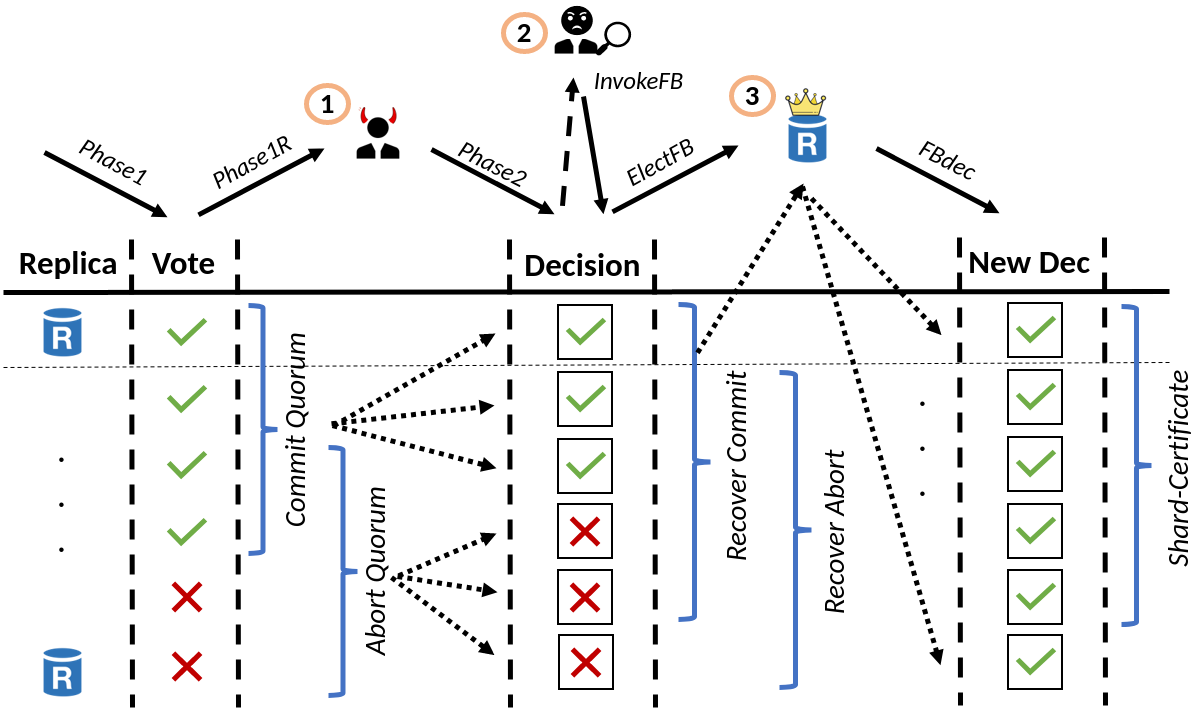
\includegraphics[width= 0.5\textwidth]{./figures/FBNom.png}
\end{center}
\caption{Fallback Scenario. 1. A byzantine client equivocates Phase2 decisions by including Commit and Abort Quorums respectively. 2. An interested client that cannot observe a Shard-decision invokes a Fallback Replica (FB) election. 3. A correct FB reconciles the decisions - A byzantine FB may repeat step 1.}
\label{fig:FigureFBnom}
\end{figure}

Figure \ref{fig:FigureFBnom} shows an example scenario requiring reconciliation, and the respective Fallback protocol message pattern.

\fs{ALTERNATIVE: Clients do not do the p1/p2 themselves, but do invocation of fallback election directly (i.e. without receiving p1r and sending p2 first). In this case replicas that elect may be missing p2 decisions and the reconciliation rule might have to issue p2 decisions based on the p1 replies included. This requires replicas to actively ignore all requests to write p2 from views < current. For seperate shard logging this is staightforward. For single shard logging however, the p2 decision requires p1 from every shard and hence every shard would need to partake in election of a fallback replica - that is messy: easier if the clients just handle it seperately.}

\fs{Optimization: (Replicas can start election right away if they have a p2). then only the first interested client had to redo p1.}
%%%%%%%
Any honest client that follows the Fallback protocol experiences \textit{Liv}. This follows straightforward from the eventual existance of an honest Fallback replica that reconciles all honest replicas. Concretely, if an honest client is interested, and the network is synchronous, at most $f+1$ fallback elections are necessary in order for a decision to be logged and for an interested client to receive a shard-decision.


We want to point out that steps 1, 2a, 3 and 4a simply correspond to the normal validation protocol. Such execution might be necessary in case the original client suffered from omission (potentially byzantine) or was simply slow (i.e. there are no inconsistencies). In order to avoid \textit{interested} concurrent and/or byzantine clients claiming power too soon and causing unecessary divergence, we grant the original client an initial window of immunity.
However, after this timer expires this transaction becomes "fair game" and anybody client can claim responsibility on termination. The orignial client too, is an interested client by default - an honest client that loses autonomy will still attempt to complete the protocol, and, if necessary elect a \textit{Fallback} itself. If the original client is byzantine, yet no other client is ever interested, a replica may eventually turn into an interested "client" itself in order to drive forward garbage collection.
Note, that it is irrelevant which client issues the $Phase1$ message. Furthermore, it is both safe and "fair" for any client to return to the Writeback phase using a Fast Path. Therefore, we enforce the timeout window only for explicit logging ($Phase2$). 

When depending on slow or byzantine transactions, clients may have to incur extra latency in order to maintain liveness. \fs{Overall, if FB invocation necessary and worst case: 1 rr voting, 3 rr FB (+1 wb) for dependencies (can be in parallel for all), 1 rr logging + 1 rr own wb.}
This is the price they pay in order to experience liveness independently from the rest of the system. On the flipside, when a clients fate is independent from other transactions, it is entirely unaffected by concurrent "view-changes". Clients that are caught equivocating or responsible for for frequent time-outs may be excluded from the system. In order to participate in a consortium database meeting performance standards is a requirement.

\fs{Fallback replicas that equivocate can be expelled. Clients that equivocate cannot be expelled because one potentially cannot tell the difference between concurrent and single client. Instead, they can get punished for being slow.}

%%%%%%%%%%%%%%%%%%%%%%%%%%%%%%%%%%%% WRITEBACK HAS ALREADY HAPPENED
\textbf{Finalized decisions:} If a replica has already received a Writeback message for a transaction it ignores all Fallback related client requests and simply returns the Writeback decision, and additionally the Writeback certificate if not yet garbage collected. A client may use either this certificate or $\geq f+1$ matching decisions to issue the Writeback for other replicas. In the following section we discuss how to perform certificate garbage collection in a manner that maintains liveness.

%-------------------------------------------------------------------------------
\subsection{Garbage Collection}
%-------------------------------------------------------------------------------
In section X (Writeback) we previously discussed how replicas garbage collect finalized \textit{Ongoing Transaction State}. \fs{A replica will eventually become an interested client in order to promote garbage collection}
We now briefly allude to garbage collecting unecessary certificates as well as outdated versions.


\fs{OVERVIEW: GC versions based on watermark. Cannot accept new tx below the watermark because lookups are expensive or either not possible anymore - unclear if sth has been gc. Must still accept ongoing TX info in order to finish them safely and consistently. Only remove commit certs once all versions have been gc in order to be able to serve reads. }


\textbf{Certificates}: Honest replicas store decision certificates for three purposes: a) It allows replicas to singlehandedly service reads (Commit Cert required) b) It allows them to singlehandedly propagate Writeback decisions to assist interested Clients and c) It allows Validation to return on Abort Fast Paths by providing conflict proofs (Commit Cert).
In theory, certificates may be removed whenever, as storing them is not necessary for Isolation correctness (the existance of a certificate implies the existance of a logged decision). Replicas  must then vote to Abstain where they previously voted to Abort (we point out that the existance of a logged decision implies that voting Abstain instead of Abort is always safe), while clients can no longer rely on single replica reads. Since certificates are comprised of signature Quorums they impose costly storage overhead and are hence important to garbage collect swiftly.

However, in order to guarantee that garbage collection is \textit{final}, i.e. no state is re-opened, we need to stricten the requirement on when to remove obsolete certificates. Concretely, we must confirm that enough replicas have finalized the decision, in order to guarantee that every interested client receives $\geq f+1$ matching decisions. \fs{Otherwise, a client might receive too few p2 decisions in order to start fallback, because finalized replicas ignore requests. In this case replicas would have to "play along" and let their decision be treated as p2. This requires re-opening Ongoing TX state, that may never be closed if there is no interested honest client} To facilitate this, we add an additional client-replica exchange off the critical path:

\fbox{\begin{minipage}{21em}
\textbf{(2: R $\rightarrow$ C)}:  Replicas receive and acknowledge Writeback decision
\end{minipage}}
Upon receiving and processing a valid Writeback decision a replica returns an acknowledgement message $EchoWB \coloneqq \langle TxID, decision \rangle_R$.

\fbox{\begin{minipage}{21em}
\textbf{(3: C $\rightarrow$ R)}:  Client aggregates acknowledgements and forwards them
\end{minipage}}
The client waits for $2f+1$ matching decisions, bundles them, and forwards them to all replicas.

\fbox{\begin{minipage}{21em}
\textbf{(4: R ($\rightarrow$ R))}:  Replica receives garbage collection confirmation
\end{minipage}}
Upon receiving $2f+1$ discrete replica confirmations a replica is aware that $\geq f+1$ honest replicas have finalized the decision and hence will assist any honest client in re-issuing the Writeback phase.

\underline{Additional subtlelties:} If a replica does not receive client acknowledgements within a time-out (a low Watermark for garbage collection has been reached), it broadcasts the $EchoWB$ message to all replicas. \fs{alternatively only forward to 3f+1 in a round robin scheme, GC as soon as $2f+1$ received}

Once a replica has achieved confidence that a Writeback is sufficiently replicated it may delete certificates. However, in order to process reads singlehandedly, an honest replica will maintain Commit Certificates until the corresponding version is gargabe collected. Next, we discuss how to prune old versions from the store.



\textbf{Versions}: We keep a shared \textit{low Watermark} that denotes what versions are obsolete. Whenever \fs{it is also fine to do it less frequent} a write (on any key) occurs, we advance the Watermark to $lowWM = localClock - \delta$. For this key, we then prune all versions $< lowWM$, with the latest version being exempt in order to maintain at least one version. \fs{periodically, we may do this for all keys in order to also prune "inactive" keys that still have multiple versions.} We point out, that client reads with $TS < lowWM$ may fail once we prune the genesis version. This does not imply transaction abort, since clients are free to change their timestamp and retry a read during execution.
\fs{we might want to abstain from transactions even if we did not prune the log, because those do not offer efficient lookups for conflicts: I.e. move the abstain logic for TX to this paragraph, and only keep dependency abstains in the log section.}

\fs{Read versions below watermark: must abstain because it is unknown whether conflicting writes were already garbage collected. Write TS below watermark: must abstain because it is unknown whether conlicting reads were gc.}
\textbf{Log Entries}: We store all committed or aborted transactions in respective Commit/Abort logs. These are un-ordered sets and allow both for fast lookup during Validation as well as offline audit off all transactions. For example, an audit on transaction reads or writes may be performed in order hold byzantine clients accountable for participation in the system. Illegal reads or non-atomic writes can be discovered and serve as Proof of Misbheavior to expell a client. When audit capability is not required, we can garbage collect old transaction decisions. We can remove CommitLog entries whenver a respective version of one of its writes (i.e. the first \fs{in this case cannot service reads below which is fine} or last \fs{would require to keep track of when the last is removed}) is pruned \fs{AND the certificate is signed off for garbage collection. Might require us to broadcast our decision (unless it was already braodcasted) in order to make sure, other tentative replicas are guaranteed to finish.}. AbortLog entries instead can be removed whenever the Low Watermark increases (need not happen on every update, but periodically) \fs{AND the certificate is set to be removed}. 

\textbf{Protocol Implications}:
In order to maintain Isolation, a replica must vote to Abstain from every new transaction with timestamp below the low watermark \fs{we may already want to do this once its removed from the store, because lookup is expensive afterwards}. Such a transactions reads and writes cannot be checked for conflicts anymore, as existing conflicts might have been garbage collected already. \fs{for reads: we can be a little more fine-grained: If there still exists a version that is smaller than the low WM, then no gc has happened yet and isolation is still safe. For writes this is not the case: cannot know whether there was a read above the write TS but below the WM that has been gc. } Additionally (for the same reason), replicas must Abstain from transactions that read versions below the watermark.
Lastly, replicas must abstain from any transaction that has a dependency with $dep.version  < lowWM$ \fs{dep version is the timestamp of such tx}, as its dependency could have been garbage collected already. \fs{in this case it would block infinitely. We can be a little more frine-grained: only need to abstain if the dep is not in the commit log. If it is, there is no need to abstain}. 

\fs{Problem: Voting abstain will still open ongoing TX state for TX that are doomed to abort. Ideally we would want to just reject the transaction outright, but then other replicas that accept the request might be stuck with it forever. This technically allows a byz client to re-issue the same TX again and again (it will always be aborted). What if now a TX that previously committed, manages to abort; this would break Consistency.
Seems to suggest: We should never GC the Logs, only certificates and versions. But GC old versions and not the log does not buy you a lot. 
Can remove the TXobject once version is gc, only keep TXid, should be cheap enough.
Could have actually done this as soon as a Writeback is received. Do not need the read/write sets anymore? all the info needed is in the store:
Maybe not true, what if somebody is waiting on a dep with ID, but does not know the whole TX.
--> can only remove tx info once "everybody" has seen the writeback, i.e. on all involved shards}

\fs{replicas would also like ignore all messages with TS below the watermark, i.e. writeback messages, fallback invocations etc. TX with incomplete state at some replicas may then never be finished... problematic: consider an example where 2f+1 replicas finish writeback and GC, but all others are still pending. they would never finish: This implies that we always need to forward to enough other replicas. (i.e. all to all, can happen in the round robin fashion)}

\fs{Would need periodic Checkpoint protocol to make sure that all replicas are on the same page what to GC and what not to accept anymore}

\fs{Maybe it is just ok to remove and reject all state below some low Watermark: since it was going to be removed anyways upon completion, it is not necessary to complete. This only matters if we do not want audit.
In theory the whole db could be stalled on any given replica and thus that garbage collection would never happen - Can just periodically increase WaterMark and gc all.}

%-------------------------------------------------------------------------------
\subsection{Optional Modifications}
%-------------------------------------------------------------------------------
Next, we discuss a series of optional modifications: \fs{not necessarily optimizations: Retries, Single shard logging, speeding up shard certificates, read leases}

\fs{we could also implement "promises" for read/write tx, in order to reduce write aborts: Delay read exec until after write happens. Can also do this on a per-client basis based on past timeliness. probably impractical though since we delay writes until validation}

\fs{Retries are a mess currently and might not be worth to include}
\fs{retries come at the cost of no fast path and having to store proofs for the transaction. These proofs are only necessary for the fallback. Moreover, it can create multiple dependencies since multi p1 remain.}

\textbf{Retries:} MVTSO, by design, favors read requests, at the cost of potentially aborting concurrent write transactions. This is intuitively sensible, as reads require additional WAN roundtrips in order to execute. 
However, when a transaction includes both reads and writes, and execution spans several reads, it becomes increasingly suceptible to abort as consequence of a conflicting read request. Observe, that aborts due a write-read conflict are a consequence of a read having failed to observe a relevant write with smaller timestamp. Thus, such an abort could have been avoided by simply choosing a larger timestamp. In order to faciliate this, we offer write transactions the option to Retry (with a larger timestamp), rather than abort. This however, comes at a tradeoff: Clients may not utilize the validation Fast-Path when opting into the availability of Retries. We outline the Retry protocol and implication for Fast-Paths as follows:

In order to be able to change the timestamp for the same transaction we must make the Transaction ID independent from it. Otherwise, it would not be possible to map retries to the same transaction in order to avoid double-commits and enable garbage collection.
Therefore, we re-define $TxID \coloneqq H(TX \setminus TS)$. A Prepare message then takes the form $Phase1 \coloneqq \langle Prepare, TxID, TX, TS \rangle_{\sigma c}$
Effectively, timestamps act as \textit{Retry Heights}: Analogous to views, only retries from a larger height can superseed previous attempts. Only the original client may retry, up to a pre-defined maximum attempts.
An honest client follows the validation protocol as previously, with the exception that it may re-do Voting phase ($Phase1$). In order to preserve Isolation, a previously Prepared transation must pass the MVTSO-Check again, as a new timestamp exposes new potential conflicts. Conflicts are not evaluated against the transaction itself at a lower height, as only a single height can ever commit.
Replicas continue to only accept the first decision they receive (maps to a single height), but must store $Phase1R$ for every retry received. This is necessary in order to maintain liveness in the presence of a byzantine or concurrent (if the original client times out) client. Interested clients may be dependent or conflicting with different heights of the same transaction and must be able to receive a $Phase1R$ Quorum in order to complete the Logging protocol. Additionally, in order to guarantee that a transaction does not commit twice for different heights, the Fast-Path must be disabled. \fs{Retries are a opt-in decision for each transaction, not for the system as whole}. When the orignial client is byzantine, or concurrent interested clients issue $Phase2$ messages, it is possible for replicas to diverge in not only their decisions, but also their respective heights. Conequently, it might be impossible for there to exist $f+1$ matching decisions from the same height. Yet, a Fallback replica must be able to safely reconcile a state. To facilitate this replicas must additionally store and include the $Phase1R$ vote Quorum in any $Elect$ message in order to prove the validity of a decision. \fs{this makes message overhead quadratic}
With this tools in hand, the updated reconciliation decision rule is simple: If there exist a Quorum of $\geq 2f+1$ matching (decision, height) pairs, preserve this pair. Othwerise choose the decision from the largest height (favoring Commit when breaking ties). This is safe, as any logged decision is preserved.

\fs{this "solution" is quite unelegant - but I suspect there might be no better way. The price for Retries are no fast path, and extra proofs. Effectively it degenerates to Indicus3}
\iffalse

- replicas keep p1s for all heights; might be necessary in case it still commits (for both safety and liveness: need to maintain isolation, need to reply with enough p1s.)
Never accept more than 1 p2, othwerise it could be committed twice.

- replicas dont accept retry prepare if they have received a p2. (might need to not do this, in order to create enough p2s for the fallback?)
- dont accept p2 from smaller height if larger p1 has been accepted. (might need to not do this, could be difficult to find the correct height)
- if a byz client equivocates p2 with different timestamps we must reconcile this in the recovery protocol. 

- cant allow fast path: then a TxId could commit/abort fast path but commit/abort slow path with 2 different timestamps. If we made the timestamp part of the ID. then we couldnt track that it is the same TX. garbage collection would be impossible and we might lose state necessary for safety.

Require proofs of p1s in the p2 decisions: because we might not get enough matching p2 ether. need to be able to decide based off just 1.

Fallback (p2 certofocates from 2 different heights cannot co-exist. if the rules for fallback dont fire, i.e. if there is none with >=2f+1 matching: choose larger height that has >=f+1 matching. Else make decision of p1s: (are included in the decision)
\fi

Enabling retries retries two modifications of the MVTSO-Check: 
First, replicas must return $RETRY, (suggestedTS)$ instead of Abstain/Abort for conflicting writes in order to allow a client to distinguish the cause of conflict. If a conflict was caused by a write, it may be resolved by attempting to commit the transaction at a higher timestamp. Naturally, this comes at the risk of additional potential read conflicts; this however, is a sensible drawback, as the transaction would have aborted in the first place. Replicas may include a \textit{suggested Timestamp} that side-steps the detected conflict. An honest client retries only, if both an insufficient number of Commit votes, but at least one Retry vote was received. \fs{Previous Abstain votes for read conflicts can potentially turn into commits, if those transactions ended up aborting}
\fs{We can keep the abort fast path with certificate for reads. This must be disallowed for writes in order to distinguish: In general, aborts with certificates require you to validate the conflict.}

Second, a transaction, whose dependencies retried, might no longer be valid. The integrity of an honest clients read transaction is violated when its dependency retries with a timestamp higher than the read. To detect this, we add additional requirement to the MVTSO-Check: $If dep \in CommitLog \land dep.TS > TX.TS:$ Return Abort/Abstain \fs{Abort with cert, Abstain without}.



Whether to opt into the availability of retries need not be a global system decision, but can be decided on a per-transaction basis. By signaling a flag within the transaction object (this changes the ID) a client can decide whether to allow for the possibility of retries which incurs the trade-off of sacrificing the opportunity of using a Fast-Path (attempts to go Fast-Path will be ignored by honest replicas if the flag is set), and additonal replica storage and bandwidth overhead (vote quorums to justify decisions) to enable live reconciliation.



\paragraph{Single shard logging}
\fs{This does not work for Atomic Broadcast!}

When transaction execution touches multiple shards validation can incur redundant explicit logging overhead. When a Slow-Path is necessary to arrive at a logged decision on S different shards, bandwith is wasted. Consider an example in which $S-1$ shards attempt to log the decision Commit, while a single shard attempts to log an Abort decision. If the latter shard succeeds, the effort of the remaining shards was in vain. 
The culprit of this phenomenon is the delayal of Two-Phase-Commit (2PC) until the Writeback phase. By preemptively making a 2PC decision \textbf{before} logging we can avoid this redundancy. We remark, that even when when all shards agree on a decision, this saves redundant coordination.
Concretely, we designate \textbf{one} involved shard as \textit{logging Shard}, while all other shards remain responsible only for Validation. Figure \ref{fig:SingleShardOpt} shows the revised structure. In order to log a decision, voting quorums from all involved shards are required. We modify step 3 of the Validation protocol accordingly:

\fbox{\begin{minipage}{21em}
\textbf{Validation (3: C)}: Client waits for vote replies from all involved Shards.
\end{minipage}}
For each involved shard, a client waits for at least $n-f$ ($4f+1$ in Indicus5) distinct replica votes, or more, up to a system specified timeout. A client aggregates a per-shard decision for each shard according to the \textit{CommitQuorum} rule. If all shard-decisions are Commit, it attempts to log a Commit decision by sending $Phase2 \coloneqq (TxID, Commit, S \times \{CommitQuorum\}$ to all replicas in the designated logging Shard. If a single shard-decision is Abort, it stops waiting for other shard-decisions and attempts to log an Abort decision by instead sending $Phase2 \coloneqq (TxID, Abort, AbortQuorum)$. 

\underline{Additional subtlelties:} A client can go Fast-Path and return to the Writeback phase immediately only if Fast-Path Quorums were received for all shards. Logging is always bottlenecked by the slowest shard. The logging Shard can be determined via a determinsitic function over the \textit{involved Shards}. A simple solution can designate the shard with lowest ID. A load balanced function could select $loggingS = min(TxID \% involvedShard)$.

The remaining Validation protocol proceeds identically to the multi-shard version. Notice, that when only a single shard is involved, no adjustments were made. The Writeback phase instead, may proceed with just the single certificate from the logging Shard: 

\fbox{
\begin{minipage}{21em}
\textbf{Writeback (1 : Coord $\rightarrow$ S)}: A coordinator receives certificate and forwards them to all relevant shards.
\end{minipage}
}
A coordinator waits for the logging shard decision, including shard-certificate, and broadcasts a $Writeback \coloneqq (TX, decision, certificate_loggingS )$ message to all replicas in all relevant shards.

The Fallback protocol is adjusted accordingly: A fallback replica need (and can) only be elected on the logging Shard, simplifying reconciliation and reducing the cost for interested clients. 


\begin{figure*}
\begin{center}
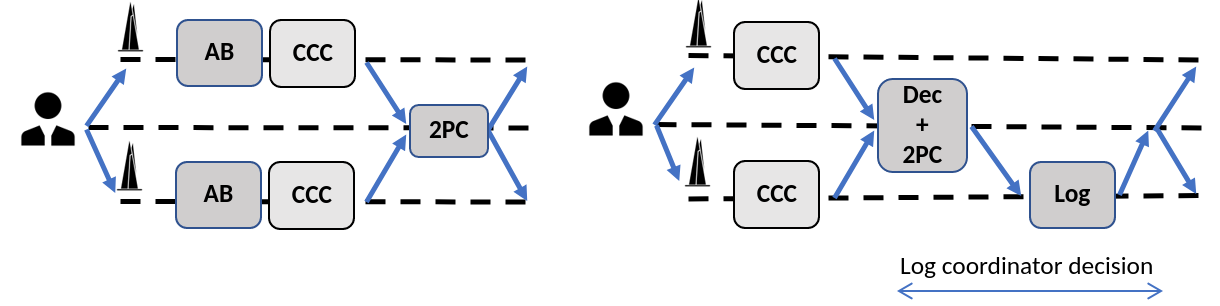
\includegraphics[width= \textwidth]{./figures/SingleShard.png}
\end{center}
\caption{Single Shard Optimization}
\label{fig:SingleShardOpt}
\end{figure*}



\paragraph{Shard decisions in asynchrony}

%%%%%%%%%%%%%%%%%%%%%%%%%%%%%%
\fs{How to get from logged decision to shard certificate: We do not implement this optimization}

When network message delays are not withing synchronous bounds an \textit{interested} client may not receive $4f+1$ matching decisions to form a shard-certificate until time-outs grow large enough. To short-circuit this wait, we can add an aditional, non critical-path, roundtrip in order to achieve liveness when tail-latencies are inauspiciousus: 
Concretely, a client may use $3f+1$ matching decisions as proof to issue a $Phase3 \coloneqq (TxID, decision, \{Phase2R_r\}$ decision message. Replicas echo this decision, and clients may return to the Writeback phase with just $3f+1$ $Phase3R$ messages. In order to maintain safety, the \textit{Decision Reconciliation Rule} must be modified. Replicas additionally report existing $Phase3$ decisions to a Fallback replica. If there exist $f+1$ Phase3 decisions we need to adopt this decision \fs{both as p2 and p3 decision is fine}. This is safe because a) no two Phase3 decisions can co-exist in the same view \fs{since 3f+1 votes must intersect in one honest}, b) the existance of a logged decision implies that any $Phase3$ message must comply with this decision, and c) the existance of a $Phase3$ certificate implies that the decision will be logged. \fs{decisions go by view precedence: phase 2 from higher view counts over phase 3 from lower view. These can be inconsistent if the decision was not logged and a p3 is generated, a view change happens without the p3 messages, and now the p3 are different from p2. But those p3 could not have been returned, otherwise f+1 would have been included in view change. Replicas dont send p3 for smaller view once new view is adopted.}
We remark, that this optimization does \textbf{not} imply that a client must wait for three roundtrips to complete, but rather may use the $Phase3R$ decisions if waiting on remaining $Phase2R$ decisions turns out to be slower. Furthermore, in a truly asynchronous network guaranteeing liveness is impossible alltogether, as a (honest) fallback replica might never be elected and consequently reconciliation might never occur.

\iffalse
\textbf{Finalized Fallbacks}
Fallback finish certificates (and do writeback themselves).\\
%%%%%%optional
\fbox{\begin{minipage}{21em}
\textbf{(6: R $\rightarrow$  FB)}:  Replicas echo decision to Fallback
\end{minipage}}


\fbox{\begin{minipage}{21em}
\textbf{(7b: FB $\rightarrow$ R)}:  FB sends p3 as final certificates. Can be writeback if only single shard involved, or if replicas know about all other shards.
\end{minipage}}



\fbox{\begin{minipage}{21em}
\textbf{(8: R }:  store certificate. use it to reply to clients that ask in the future if necessary.
\end{minipage}}
%%%%%%%%%%%%%%%%%%%%%%%%%%%%%%%%%5
\fs{END}
\fi



\paragraph{Personalized Read Leases}: 
Read Timestamps allow executing read transactions to tentatively acquire additional commit confidence by avoiding concurrent write conflicts to manifest. However, this opportunity also empowers byzantine participants that may acquire read timestamps \textit{without} ever intending to commit a transaction. Unlike committing transactions, that are guaranteed to be eventually logged and audited (if it pertains to honest participants interest), there is no point of accountability for such behavior. It is indistinguishable from arbitrarily long executing transactions and would require explicit additional logging efforts. In order to avoid targeted abuse, we re-iterate the rationale of \textit{expecting} timely client performance. Clients that are untimely are, to the system, no better than malicious actors and need to be excluded for performability purposes as the scalability of Indicus is directly related to the industriousness of clients. 
We point out, that a persistant Read Timestamp only implies that write transactions with smaller timestamps may abort. As time moves on, old Read Timestamps become obsolete as new writes no longer conflict. The objective is therefore limit the repetitiveness of such behavior.
Since Read Timestamps are not necessary for safety, they can be granted both as temporary lease and on a per-client basis. Read Timestamps that are evaluated for conflicts past their \textit{Expiration Time} are ignored. This can be implemented in a straightforward fashion by re-defining Read Timestamps $RTS \coloneqq (TS, exp )$, where exp is an expiration time assigned by the replica $exp \coloneqq R.localClock + \Delta_c$. An RTS is only valid during the MVTSO check if $localTime < exp$. The offset $\delta_c$ can be tuned for each client indivdually, based on its past timeliness; Untimely clients may eventually be granted no Read Timestamp, or, be exlcuded from the system.
\fs{ALTERNATIVE: We grant only limited Read Timestamps by redefining $RTS \coloneqq clientTS - \tau_c$, where $\tau_c$ is a defense treshold for each clients reads. The threshold is initialized to zero ($\tau_c \leftarrow 0$), and grows (or shrinks again) based on client untimeliness. Thus, RTS initially grants read protection against all writes with $write.TS < read.TS$, but eventually protects only against $write.TS < read.TS - \tau_c$ (i.e. slow clients are granted smaller protection window against concurrent transactions).}



%%%%% OTHER
\textbf{Tolerating High Skew}
Use Waits at replicas to re-order in timestamp order
Use write promises (replicas wait for certain writes to arrive before processing reads).


\textbf{Exponential Backoff}
When there is contention one might need exponential backoff in order for one transaction to eventually succeed. Cannot rely on clients to enforce this because they may be byzantine. Replicas must keep backoff list for each client.
Open question: When to reset to 0? Upon success? This would mean that a single client could get lucky many times in a row. More likely: reset after some k amount of tx have passed? But then those could be byzantine and never attempt to commit. --> Reset after some timeout.


\textbf{Limit concurrent transactions}
Would like for byz clients to only do k transactions concurrently (probably k=1). We could either enforce this pro-actively using a ticket granting service (like the timestamp generation phase), but that would induce additional overhead. Or: we could make it an incentive. If replicas receive another request from the same client before the last one has finished they abstain from it and report the client (just like multi retries). An honest client is going the be an interested client for its own transaction if it loses control. Hence it is reasonable to assume a client only starts another TX after it has finished its last one. Can use per client sequence number to enforce FIFO on its own transactions.

\textbf{Threshold signatures}
Can use threshold signatures to reduce message sizes and replica validation overhead. This however induces significant additional client overhead to compute TH sigs. Only worth it when replication degrees are high (see SBFT)

\textbf{Merkle trees for smaller write certificates}
currently a certificate is a signature for a committed TX. this means that a read must return the whole TX that wrote the value instead of just the value. Could reduce this by using a merkle tree for signatures that reduces cost.
Replicas sign not only the TX, but also a Merkle Hash Root of all the Writes. Then only log(|writes|) writes or intermediate hashes are necessary to prove legitimacy of write value.
--> Result: smaller read reply messages, but bigger protocol messages because double sigs required. Probably not worth it.

\iffalse
\textbf{Reduce tx object content per shard.}
\fs{Each shard should only store the objects necessary for its shard: changes ID.
keep track of not just involved shards, but of involved sub TXIDS: Each shard involved has a different TXID: Each sub TX object includes a list of the other TXIDS. An honest client experiences atomicity by bundling - doesnt work straightforward because cyclic. Need 2 levels of ID. Problem still remains: Byzantine client could fake which sub IDs to wait for. These may not exist and hence liveness would be impossible.}
\fs{can reduce lookup time by splitting into per shard read/write sets. But full info still necessary for recovery}
\fs{In order to facilitate recovery just based on IDs, replicas must be allowed to vote abstain. In this case, they may only vote after a timeout to provide the orignial client with a window of immunity. If the TX does exist, and a replica has it, it can forward it to the client who can use it to attempt to commit. It is still undesirable because a byz client can claim limitless false components (and hence always make its TX abort). If an interested client cannot acquire the Tx contents after the timeout (and a replica has not seen it) it can try to convince the replica that the orignial client was faulty. So when this happens too often, a client can be expelled. A byz client can abuse this by always saying this about any honest client; but if that client was timely, then the replica would have known about the TX!}
\fi

TODO:

\textbf{Fallback less load for single sharded logging}

\paragraph{Hierarchical transaction IDs.}
When transactions span multiple shards, the resulting transaction object includes ReadSet, WriteSet and dependencies from different involved shards. Consequently, every involved shards must validate, and store keys/values from all shards (potentially the whole database) instead of only keys assigned to the respective shard. To circumvent this, we split the transaction object into multiple sub-objects that pertain only to the respective shard, shown in Figure \ref{fig:FigureTxId}. Each sub-object $TxS_j$ has an individual identifier $id_j = H(TxS_j)$ that represents the involved shards of a transaction. A $TxID = H(involvedShards, TS)$ serves as common identifier of the transaction across all shards.

\begin{figure}
\begin{center}
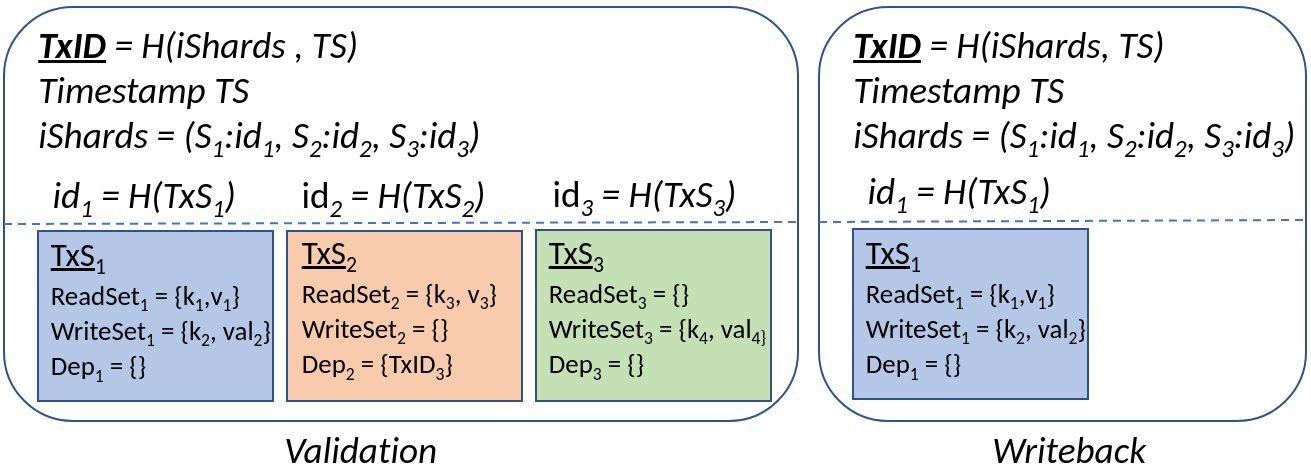
\includegraphics[width= 0.5\textwidth]{./figures/TxIDs.png}
\end{center}
\caption{Logging}
\label{fig:FigureTxId}
\end{figure}

During Validation, client send the entire transaction object to each involved shard. This allows replicas from any shard to aid recovery, in case a malicious client never sends the request to every involved shard. \fs{If we didnt have the full TX, we would be forced to abort sub transactions that have never been sent which would allow byz clients to always abort themselves}
 A replica in shard $S_1$ checks, whether all $TxS_j$ match their digest $id_j$, whether every $TxS_j$ maps to an involved shard, and whether all involved Shards match the $TxID$. It then performs the MVTSO-check only for $TxS_1$. If $TxS_1$ contains a key that does not belong to $S_1$ this serves as PoM \fs{a byz client messed up}. 
For Writeback, it suffices for clients to send only the sub-object $TxS_j$ relevant to shard $S_j$. Since a valid Writeback message must include a shard-decision for each involved shard, it is implied that every shard has durably replicated the Validation transaction object. Thus, it is no longer necessary for shard $S_j$ to keep track of $TxS_i$ ($i \neq j$) for liveness purposes \fs{the other shards contain the info themselves}, and it may store only the objects relevant to its shard. A replica can validate the legitimacy of $TxS_j$ by recomputing $id_j$ and comparing to the signed instance in the shard-decision.\\
 



\textbf{Strict Serializability}
Read Latest

\textbf{Retries v2}
Retries for different ID:

Protocol:
Client receives 3f+1 Abstain/Retry votes. If 2f+1 of those are retry (implying that there could be 3f+1 commit votes) a client retries:
1. Aborts the orignial slot on the fast path
2. Commits new version with new timestamp. New ID must be old ID, bar timestamp change. (Other TX are rejected - this avoid multiple TX per client)

Comments:
1. Byz client may just commit same TX twice. That is safe, since Tx needs to pass validation check at 2 times. The higher TX strictly dominates the lower TS. Conflicts are from read.version up to TS.
(Abstains never change? Only retries and commit do)

2. Dependent will be aborted. (TS does not match dep read version anymore) This is fine, since the dependent would have been aborted anyways. Is there a way to "save" the dependents too?

%-------------------------------------------------------------------------------
\subsection{Indicus3}
%-------------------------------------------------------------------------------
When a replication degree of $n =5f+1$ is deemed too costly, an application can defer to the use of Indicus3. Indicus3 requires the optimal number of replicas $n = 3f+1$ in order to tolerate byzantine faults, at the cost of several design trade-offs.

First, Indicus3 cannot experience a Fast-Path for Committing transactions as it is impossible to log a Commit decision based on the votes alone. Since Indicus3 uses fewer replicas, we adjust Quorums sizes accordingly: any protocol Quorum must contain $2f+1$ replicas (where previously we chose either $4f+1$ or $3f+1$). Only if Commit votes are unanimous can we proceed to log a Commit decision. This is necessary to maintain Isolation guarantees through Quorum intersection (for any two Quorums, they have at least one honest replica in common). Even when $3f+1$ replicas vote to Commit, a later interested Client (or a byzantine client attempting to equivocate) might observe only $f+1$ commit votes since it cannot reliably wait for Quorums of size $\geq n-f$. Thus, there may be no Fast-Path. 

Second, logging a decision requires both an additional round-trip, and certificate overhead in order to guarantee that reconciliation maintains SAF. To convey the intuition behind this, consider the following example where $2f+1$ replicas returned $Phase2R$ decision Commit, and the $f$ remaining replicas are both honest and decided Abort. Any Fallback replica charged with reconciliation must be able to make a decision based on $n-f = 2f+1$ decisions. However, in the presence of byzantine replicas, the observed Quorum might only contain a single Commit decion and $2f$ Abort decisions. No conclusive reconciliation can be made as it is indistinguishable what decision might have been "logged". To break this stalemate, we must introduce an additional phase $Phase3$: A decision is only logged, when $f+1$ honest replicas adopts a $Phase3$ decision, and $2f+1$ matching $Phase3R$ messages are necessary in order to form a shard-certificate. A $Phase3$ message respectively requires the endorsement of $2f+1$ matching $Phase2R$ messages. Thus, by Quorum intersection, it is impossible for two different legal $Phase3$ decisions to co-exist. To maintain SAF, it must moreover be possible to recover a logged decision based on a single $Phase3$ decision. This in turn implies, that decisions must include the $Phase2R$ Quorums as proof to maintain Isolation integrity. The fallback reconciliation rules must be extended accordingly. Note, that a $Phase3$ decision might never exist if $Phase2$ decisions are not consistent. Therefore, the orignial reconciliation rules must be preserved, with precedence given to $Phase3$ decisions, if existant.

These trade-offs are reminiscent of the additional overheads required to offer Retries. In fact, Indicus3 inquires no additional cost to provide Retries as Indicus3's modification satisfy the same functionality.

We point out, that while Indicus3 incurs additional round-trips compared to Indicus5, total latency is not necessarily higher, as Indicus5 relies on larger Quorums and is hence gated by higher-tail latency.
To nevertheless reduce the gracious execution latency we can modify Indicus3 with either one of the  two optimizations options outlined below. Neither of these optimizations are compatible with Retries however:
\textbf{Option A:} We can offer a $Phase2R$ "Fast-Path", by allowing a shard-certificate to be formed on the basis of $3f+1$ matching replies. The existance of such a certificate implies that any $Phase3$ decision must comply. Further, in absence of any $Phase3$ decision, it is possible to reconcile a decision consistently by recovering a decision if $f+1$ Phase2 decisions exists.

\textbf{Option B:} When byzantine participants do not comply or the network is asynchronous, receiving $n =3f+1$ matching replies may be impossible. Nevertheless, we can allow Commit decisions to form shard-certificates within just two roundtrips by denying Abort decisions this possiblity. By introducingaAssymmetry to the protocol, it is possible to safely recover based on a single $Phase2$ Commit decision. This introduces additional cost for Abort decisions as they must complete an additional $Phase3$ in order to complete. \fs{commits will also always get a shard certificate by doing another phase if necessary}. The reconciliation rule must be adjusted accordingly in hierarchical fashion: A single $Phase3$ Abort decision takes precedence over a single $Phase2$ Commit decision, which in turn takes precedence over an arbitrary recovery. This is safe, as a Commit and Abort Shard decision cannot co-exist as they each must have been established on the premise of $2f+1$ $Phase2$ decisions. 
Adding additional cost for Aborts is sensible if the application expects conflicts to be rare. In this case Commit decisions form the common protocol operation, and are optimized accordingly. Note, that the role of Commit and Abort can be interchanged trivially.

Lastly, we want to remark that Indicus3 offers weakened Byzantine Independence guarantees. Concretely, it is possible for a byzantine client to determinsitically abort its own transactions by only relying on vote Quorums that include a colluding byzantine replica. Thus, honest transactions that claim respective dependencies are exposed to the whim of byzantine clients. This can be circumvented only by declining to ever accept dependencies.

\iffalse
3f+1 if not defending against byz colluders as much

- due to indistinguishability, no fast path
- Commits in 2 rounds, Aborts in 3 (Alternatively symmetric version)
- decision quorums and fallback quorums change accordingly.
- proofs necessary for recovery (like for Retries) --> retries add no additional cost to Indicus3
- recovery rules change, similar to The phase 3 optimization for shard decisions
\fi

\iffalse
\begin{figure}
\begin{center}
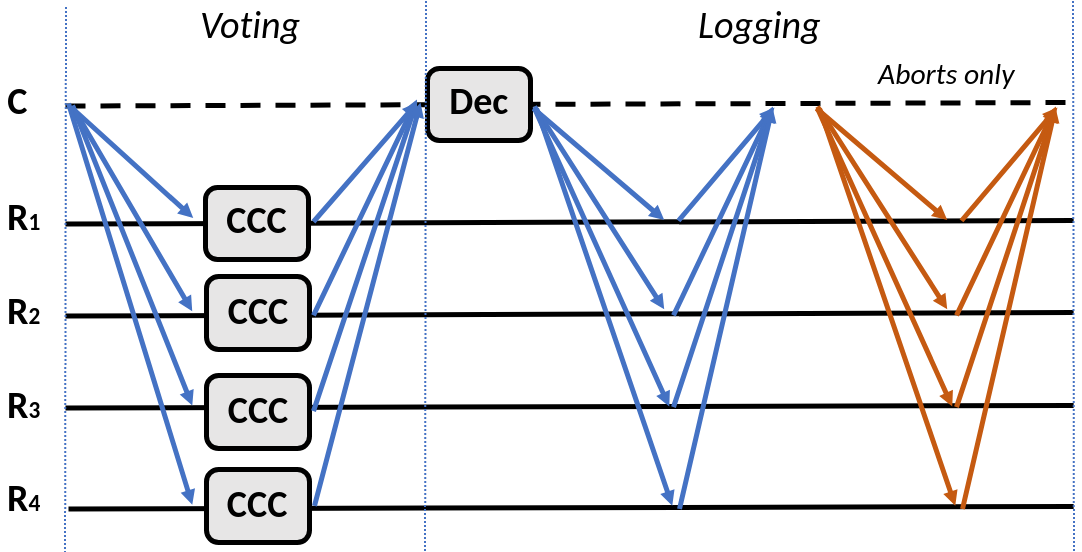
\includegraphics[width= 0.4\textwidth]{./figures/3f+1.png}
\end{center}
\caption{Logging}
\label{fig:Figure1}
\end{figure}
\fi


%%-------------------------------------------------------------------------------
\section{Discussion}
%-------------------------------------------------------------------------------
1. Explain or prove how we satisfy byzantine independence and why we want it:

byz participants cannot reactively make aborts happen if they do not control the network. 
This is stronger than a leader based setting.  A byzantine leader can always reactively create a conflicting TX. An honest leader would not do this. 
Thus we are equivalent to an honest leader.

(If you know the keys beforehand it is possible to create mutually aborting transactions to form dependencies. But this requires additional knowledge; arguably dependent on the network too).


2. Can use witnesses instead of full replicas to reduce replication cost. Those need to only contain key/version and no values.






%-------------------------------------------------------------------------------
\section{Implementation and Evaluation}
%-------------------------------------------------------------------------------

\subsection{Experiments}
-Comparison vs Tapir
-Evaluation of the signature and proofs overheads.
-(Evaluation of performance under view changes: should show that its not affected too much)
-(Comparison against our own system but with Validation doing Atomic Broadcast)
-(Comparison against Hyperledger?)


%-------------------------------------------------------------------------------
\section{Limitations}
%-------------------------------------------------------------------------------
Shifting responsibilites from replicas to clients comes at the cost of higher computational requirements for clients which may not be tolerable for some applications that demand lightweight clients \cite{gueta2018sbft}. In practice, we envision \sys clients to be dedicated transaction managers, that provide an interface for light-weight end-users. 

As is inherent to any system leveraging optimistic concurrency control, \sys is vulnerable to highly congested workloads and must yield the abort of some transactions to maintain isolation guarantees. Note however, that when clients conduct transaction execution, a pessimistic, locking-based concurrency control (i.e. 2PL) incurs deadlock resolution on the same order of frequency, yet requires additional coordination overhead. Speculative execution however, is inherent to an interactive interface; applications striving for deterministic committability must restrict their transaction model and/or rely on serial execution (i.e. SMR). 

Similarly, as is the case for most BFT protocol, \sys is vulnerable to ddos attacks by byzantine participants. A byzantine client with unrestricted access control may subverting progress for honest users by artificially increase congestion. Defense against fllod-based attacks is out of scope of our work, but is disincentivised as participants are accountable in permissioned membership groups. We remark that clients in \sys can deterministically abort transactions (byzantine independence) only when controlling the network.



\iffalse

Shifting responsibilites from replicas to clients comes at the cost of higher computational requirements for clients. This may not be tolerable for some applications, and other existing systems (i.e cite sbft) structure their design explicitly to be compatible with lightweight clients. In practice, we envision Indicus clients to be dedicated transaction managers, that provide an interface for light-weight end-users. For example, in a distributed stock market, brokers may act as transaction managers in lieu of their clients.

As is inherent to any Optimistic Execution and Concurrency Control, Indicus is vulnerable to highly congested workloads. When contention on select objects is high, concurrent execution of Transactions must yield the abort of some Transactions during Validation in order to maintain the Database Isolation guarantees. 
\fs{When contention is very high, it can be desirable to in fact have a total order. Doing just validation in total order wont reduce aborts though. Requires transactions to be pre-defined }

Note however, that when clients are in charge of execution, a pessimistic concurrency control solution such as two-phase-locking would incur an equal amount of deadlocks which would require resolution. The observation to make is that any system that conducts execution at the client application side speculates on concurrency. This however we stipulate, is unavoidable when trying to scale a system to the number of users rather than replica processing power. The traditonal ways to avoid the abort rate conundrum is to either restrict the transaction model, which in turn weakens the general applicability of the protocol, or to delegate execution to replicas and utilize State Machine Replication to serialize Transactions. SMR protocols with a single leader do not inquire any congestion based aborts as a single sequencer naturally eliminates concurrency.
Indicus does not make these concessions in order to offer interactive Transactions and remain scalable. A workload that exhibits low commutativity and high contention should therefore refrain from adopting our system.

Similarly, as is the case in any transaction protocol, Indicus is vulnerable to ddos attacks by byzantine participants. A byzantine clients only opportunity at subverting progress for honest users is to artificially increase congestion. When such a client has unrestricted access control it may do so strategically iff it has control over the network. If it does not, it cannot reliably gain knowledge about concurrent transactions before they pass the validation step and must resort to flooding based attacks. Defense against such attacks is out of scope in our work, but is disincentivised as participants can be held accountable for their actions in a closed membership setting.


\fs{technical limitations: We require more replicas to avoid certificate signature overheads. Since in 3f+1 one decision needs to be enough to recover. byzantine replicas/clients have more power to vote arbitrarily, because they cannot be held accountable for it. In total order protocols (SMR), deviation from the "common" vote signals misbehavior, whereas for us that is not the case. --> this should go as a challenge somewhere.}

\fs{Clients are more heavyweight. Not suitable for settings where clients just have minimal processing capacity. In practice we envision clients to be dedicated transaction maangers.
Also, Clients need to be registered in system with a sig - necessary to enforce access control in any system however}
\fi


%-------------------------------------------------------------------------------
\section{Related Work}  
%-------------------------------------------------------------------------------

\paragraph{Consistent Replication}
Indicus offers a replicated, byzantine fault tolerant database that leverages concurrency control and quorum based agreement to maintain isolation guarantees despite its unordered/inconsistent replication layer. 
The majority of prior work instead maintains consistent replication by means of the State Machine Replication (SMR) approach \cite{schneider1990implementing}. Existing replication solutions for the crash failure fault model (Paxos based: \cite{Li2007, Lampson2001, Lamport98Paxos, Lamport2005a, Lamport2005, Lamport01Paxos, Chandra2007} , Zab: \cite{junqueira2011zab}, \cite{van2014vive}  VR: \cite{oki1988viewstampeda, liskov2012viewstamped}, Raft: \cite{ongaro2014search}) as well as the byzantine fault model \cite{lamport2011byzantizing, pires2018generalized, Guerraoui08Next, Kotla04High, bessani2014state, liskov2010viewstamped} (most notably PBFT \cite{castro1999practical}) maintain consistency by achieving consensus on a totally ordered log of requests. They are, in addition, primarily leader-based which introduces additional scalability issues~\cite{epaxos,tapir} as well as fairness concerns. Recent efforts to address this bottleneck can be classified in three ways. Then you have your enforcing PO, fine-grained ordering, sharding}

The seminal \textit{practical} Byzantine Fault Tolerance (PBFT) protocol and its adaptations (cite Zyzzyva, aardvark..) form the cornerstone of most Permissioned Blockchains \cite{Hyperledger, EthereumQuorum, buchman2016tendermint, al2017chainspace, kokoris2018omniledger,  gilad2017algorand, baudet2019state} (Algorand and Omniledger both not permissioned, but lots of PoS blockchains elect validator set that runs pbft basically, mention some traditional blockchains? Bitcoibn, Ehtereum, also total order).

\fs{mention zyzzyva explicitly because of Fast path concept and speculative execution of replicas. Difference: still leaderbased and clients EXPECT replicas to process in order.}


\paragraph{Enforcing Partial Order}
Totally ordered ledgers solve the problem of consistent transaction replication but enforce unecessary coordination/serialization between commutative operations. 
Approaches to reconcile this scalability limitation by inducing only a partial order can be broadly categorized in three ways:
\textbf{1. Fine-grained ordering}: One class of approaches attempts to only order conflicting operations by leveraging transaction semantics. Existing work however (cite all CF: Epaxos, Generalized Paxos, \cite{sutra2011fast}, \cite{li2012redblue}, Curp, Carousel, MDCC, Tapir, Janus) targets almost exlusively the crash failure model. To the best of our knowledge, Bilbos/Clairvoyant is the only BFT system that offers SMR for commutative transactions, but unlike Indicus is limited to a static transaction model and introduces blocking, as any transaction must wait for all potentially concurrent transactions to complete. Other quorum based systems whose strucutre Indicus resembles (Q/U, H/Q, Liskov rendering harmless) allow for commutativity, but do not offer transactions. \fs{Q/U resembles Logging in Indicus - but has no liveness on its own.}

\textbf{2. Sharding} In the blockchain space, sharding has been explored as mechanism to parallelize independent transactions across shards, while relying on total-order primitives within (Omniledger, Chainspace); In Indicus we argue however, that inducing a partial order via sharding is merely a limited engineering optimization. Existing work in the crash failure model (Tapir, Ordering Paper, Janus) points out that layering sharding and transactional control on top of replication (cite Spanner?) incurs redundant coordination, and improves performance by integrating both layers. Indicus is the first to adopt this rationale in the byzantine fault model.

\textbf{3. DAGs} Lastly, the use of Directed Acyclic Graphs (DAGs) that allow to parallelize agreement instances, has been explored in several permissionless blockchain networks (Iota, Byteball, Ava, overview paper). It remains unclear whether practical applications exist for the permissioned setting - designing a BFT protocol that replicates a DAG instead of a totally ordered ledger is an interesting avenue for future work.


\paragraph{Byzantine Databases}
In Indicus we argue that blockchain functionality, i.e. a distributed transactional system, should be captured by a BFT Database (DB). There exist a series of work offering explicit BFT DBs  
cite( Byzantium, Augustus, Callinicios, HRDB, BFT Dur, Databasify Fabric): HRDB offers interactive transactions for a replicated DB, but relies on a trusted shepherd layer. Byzantium designs a middleware system that utilizes PBFT as atomic broadcast (AB) and provides Snapshot Isolation via a primary backup validation scheme. In cite(BFT Dur) Pedone et al. too, rely on AB to design an OCC-architecture similar to Indicus. Augustus and Callinicos leverage sharding for scalability by assuming a limited comparison/query/update transaction model and implementing an optimistic and locking based execution model respectively on top of atomic broadcast.
We expand on existing research to 1) be leaderless and more scalable by allowing un-ordered replication rather than AB, 2) provide interactive transactions, and 3) offer sharding for horizontal scaling.
\subparagraph{Byzantine Clients}
Existing work concerned with byzantine clients addresses mechanisms to reduce frequency and severity of client misbehavior (BFT-dur, byzantium, agustus, callinicos, others, byz liskov). We reformulate transactional corectness guarantees in a byzantine setting to be more explicit about byzantine client behavior \fs{too vague} and extend Liskov et al.s (cite rendering byz client harmless) definition of Byz-Linearizability to transactions (Byz-Serializability). 
Lastly, Herlihy (cite) discusses mechanisms to improve fairness in leader-based systems - In Indicus we sidestep fairness concerns by being leaderless and instead define Byzantine Independence in order to formalize byzantine influence.











\subsection{details}


Indicus is the first to do blablabla. This section describes related work...

\textbf{Distributed Transactions for benign faults}
A lot of recent effort has gone into designing high throughput and low latency databases that leverage synergies between transaction and replication layer to improve performance. The recently proposed TAPIR transaction protocol leverages redundancy between transaction ordering and replication ordering to reduce total roundtrips, thus reducing latency in wide area networks. TAPIR shares several similarities with our system, most notably the absence of a leader and the resulting unordered validation structure. Like Indicus, TAPIR utilizes optimistic concurrency control to allow for concurrency among commutative transactions while minimizing coordination. When congestion is high however, throughput and tail latency worsen as abort rate grows. Janus avoids transaction aborts by dynamically re-ordering conflicting transactions \cite{mu2016consolidating}. This however, is made possible by assuming one-shot transactions, i.e. fixed read/write keys, and thus reduces the application generality. Another key-value store, Carousel, similarly assumes a restricted Transaction model in order to parallelize execution and validation \cite{yan2018carousel}. CURP too, leverages commutativity in order to reduces replication costs by making requests durable first, and only ordering them later \cite{park2019exploiting}. 

While all of these databases offer low latency replication, they are fundamentally limited to tolerating crash-failures. This strong failure assumption makes them less robust and not suitable for mission-critical services \cite{Abdollah2007}, finance or otherwise highly sensitive data.

\textbf{Byzantine Fault Tolerant Replication} 
\fs{Really not necessary to explain all the different SMR protocols that exists. Rather: Should explain how they could be used to solve the same problem with total order?}
 The problem of tolerating arbitrary failures was originally formalized as \textit{Byzantine Generals Problem} \cite{lamport2019byzantine}, paving the way for countless Byzantine Fault Tolerant (BFT) protocols and implementations \cite{castro1999practical, martin2006fast, kotla2007zyzzyva, pires2018generalized, bessani2014state, lamport2011byzantizing, arun2019ezbft, malkhi2019flexible, duan2014hbft, yin2003separating}. Such protocols have a reputation of being  both notoriously difficult to understand and design correctly \cite{abraham2017revisiting, abraham2018revisiting, shrestha2019revisiting}, and in practice often impose significant overhead compared to its crash-failure tolerant counterparts, hence limiting frequent industrial adoption.
Recently however, with the surge in Blockchain interest, BFT protocols are experiencing a second Spring. While originally developed to tolerate arbitrary bugs, these protocols find increasing importance in settings where participants are untrusted or malicious. Permissioned Blockchains, organized by a consortium of registered participants can use traditional BFT State Machine Replication (SMR) protocols in order to achieve agreement. 
\fs{mention basic BFT first? pBFT is the first "practical", not the first BFT}
The seminal practical BFT (PBFT) protocol \cite{castro1999practical} implements a primary backup scheme that achieves consensus in three broadcast rounds, maintaining safety as long as the number of faulty participants is $<1/3$ (i.e. $n\geq 3f+1$), and offering liveness during synchronous operation. When primaries misbehave, a dedicated \textit{view-change protocol} allows for safe reconciliation. There have been numerous adaptations that aim to speed up common case and failure free execution such as FaB \cite{martin2006fast}, and most notably Zyzzyva \cite{kotla2007zyzzyva} which leverages speculative execution and a semi-client driven protocol to reduce latency. Akin to Indicus, replicas in Zyzzyva speculatively execute requests out-of-order, and rely on honest clients for reconciliation. Zyzzyva replicas however, \textit{expect} to process requests in-order, and diverge only temporarily as result of a byzantine leader. hBFT builds on Zyzzyva and attempts to improve faulty case behavior by returning the client responsibility of detecting inconsistencies to a dedicated replica checkpointing protocol. 
UpRight explores efforts to tolerate both byzantine and crash failures in order to make the overhead of deplyoing a BFT system practical.
SBFT \cite{gueta2018sbft} pursues the goal of scaling to scale to large replication degrees, while offering light clients and high throughput under benign faults. It adopts the UpRight replication model, and modifies PBFT by utilizing collectors, threshold signatures and a fast path akin to Zyzzyva. 
Aardvark \cite{clement2009making} emphasizes the importance of robust performance under byzantine failures by adding increased client and replica checks and imposing frequent leader rotation by steadily increasing throughput requirements. Tendermint \cite{buchman2016tendermint} pushes this idea to the extreme by rotating leaders continuously, at the cost of assuming a synchronous network. Herlihy and Mor attempt to rigorize fairness properties for permissioned Blockchains and propose techniques to increase accountability for Tendermint specifically \cite{herlihy2016enhancing}.

HotStuff too, explores the use of rotating leaders by exploiting the symmetry in PBFTs phases in order to pipeline transaction processing \cite{yin2019hotstuff}. 
Nevertheless, all protocols derived from the PBFT family suffer from the leader bottleneck as well as enforcing a total order even on commutative operations. BFT-Mir \cite{stathakopoulou2019mir} identifies the proposal speed of a single leader as the practical bottleneck in most implementations and improves upon this by allowing all replicas to act as proposers.
Biblos \cite{bazzi2018clairvoyant} achieves leaderless SMR by leveraging a non-skipping timestamp protocol. It furthermore allows for commutative transactions to be executed in parallel at the cost of requiring read/write key sets to be known in advance. In order to preserve liveness however, Bilbos falls back to a PBFT resolution. \fs{Uses all to all, predefined TX, pbft fallback, timestamp phase and proofs required}
The Quorum/Update (Q/U) protocol too, offers leaderless agreement by leveraging Qurorums for a agreement in a limited read/write interface, but fails to terminate under contention \cite{abd2005fault}. To reconcile this shortocming, the Hybrid Quorum protocol (HQ) explores a hybrid solution, extending upon Q/U by adding a PBFT fallback path under contention \cite{cowling2006hq}. In \cite{liskov2006tolerating}, Liskov et Al explore improved byzantine Quorum protocols for a single Read/Write interface, giving special attention to bounding the effects of byzantine clients. 
\fs{BFT protocols under fire: \cite{singh2008bft} that one-size-fits-all protocols may be hard if not impossible to design in practice}
All of the above systems, including Indicus, guarantee Liveness only under the assumption of some degree of synchrony. This is consistent with the well known FLP impossibility result stating that no deterministic consensus solution may exist in the presence of asynchrony \cite{fischer1985impossibility}. Protocols such as Ben-Or's algorithm \cite{ben1983another}, HoneybadgerBFT \cite{miller2016honey} or BEAT \cite{duan2018beat} sidestep this result by introducing randomization, thus enabling probabilistic agreement even during asynchrony.

\textbf{BFT distributed transactions}
While the literature on BFT state machine replication is extensive, the efforts to offer a transactional interface for BFT are scarce. SMR itself can be utilized as a straw-man system to implement pre-defined Transactions (one-shot or stored procedures) by enforcing a common total order in which replicas will execute the transactions. \fs{Byz agreement apps for DB \cite{garcia1986applications}}
HRDB offers a dedicated BFT Database, but assumes a trusted shepheard layer, thus not being truly BF resilient \cite{vandiver2007tolerating}.
Byantium \fs{middleware stuff} offers Snapshot Isolation for Transactions by re-purposing PBFT as atomic broadcast. It executes requests only at a primary and uses replicas to validate results in the total order defined by the SMR protocol \cite{garcia2011efficient}. Augustus implements short-transactions, a limited, comparison/query/update transaction model that declares all operations before execution \cite{padilha2013augustus}. It offers scalability via partitioning and achieves consistency within partitions by utilizing atomic broadcast. While Augustus assumes an optimistic execution model that allows for aborts under concurrency, its follow up work Callinicos implements a locking scheme in order to avoid Transaction aborts \cite{padilha2016callinicos}. To do so efficiently it resorts to a limited transaction model that requires knowledge of read/write sets and otherwise locks an entire partition in order to guarantee mutual exclusion, thus voiding any concurrency. BFT Deferred Update Replication adopts an interactive OCC transaction model comparable to ours, allowing execution to be speculative at clients \cite{pedone2012byzantine}. However, it uses PBFT as atomic broadcast implementation to enforce SMR on validation, thus resorting to both a leader, and a total order on all requests. It moreover does not extend to multiple shards.

\textbf{Blockchains and Sharding}
In the Blockchain world, Chainspace \cite{al2017chainspace} and Omniledger \cite{kokoris2018omniledger} implement sharding by layering 2PC and atomic broadcast (within shards) for the UTXO transaction model. Rapidchain \cite{zamani2018rapidchain} offers efficient sharding for a permissionless system (what else? didnt read much, not so relevant). Hyperledger provides an enterprise-ready permissioned blockchain solution that simulates optimistic transaction processing by letting replicas speculatively execute Smart Contracts. While Hyperledger \cite{Hyperledger} describes itself as a shared database, it relies on a dedicated SMR ordering service that enforces a total order, and, in practice, only tolerates crash failures (Hyperledger uses Raft \cite{ongaro2014search}, a consensus protocol for the Crash-Failure model,  but can be extended to use PBFT). Sharma et al. attempt to \textit{databaseify} Hyperledger by adding database techniques such as transaction re-ordering in order to reduce aborts, but fundamentally maintains the totally ordered (Hyper-) ledger design \cite{sharma2018databasify}. \fs{Databasify paper: tries to add some bandaid db techniques to hyperledger. Transaction re-ordering (still total order), and early aborts.} 
 \fs{(Mention other Permissioned Blockchain systems: Ethereum Quorum? (uses Raft or IstanbulBFT = implementation of pbft)}

Directed Acylcic Graph (DAG) based consensus architectures \cite{pervez2018comparative}(IoT-chain, IOTA, Byteball - all are blockless) have been explored  in order to parallelize agreement and execution instances. While these approaches increase throughput by inducing a partial order, they target permissionelss settings (based on Proof of Work/Stake), rather than permissioned BFT-based solutions. To the best of our knowledge there exists no such system to this date, and it is unclear how to merge these approaches. Designing a BFT protocol that replicates a DAG instead of a totally ordered ledger is an interesting avenue for future work.






\fs{How does all this related work compare to Indicus?}




%-------------------------------------------------------------------------------
\section{Conclusion}
\label{section:conc}
%-------------------------------------------------------------------------------

summary of Indicus

Our experience designing Indicus.

opportunities for future systems? what kind of systems maintain the defs?

\iffalse
%-------------------------------------------------------------------------------
\section*{Acknowledgments}
%-------------------------------------------------------------------------------

The USENIX latex style is old and very tired, which is why
there's no \textbackslash{}acks command for you to use when
acknowledging. Sorry.

%-------------------------------------------------------------------------------
\section*{Availability}
%-------------------------------------------------------------------------------

USENIX program committees give extra points to submissions that are
backed by artifacts that are publicly available. If you made your code
or data available, it's worth mentioning this fact in a dedicated
section.
\fi
%-------------------------------------------------------------------------------
\bibliographystyle{plain}
%\bibliography{ref}
\bibliography{refs}

%%%%%%%%%%%%%%%%%%%%%%%%%%%%%%%%%%%%%%%%%%%%%%%%%%%%%%%%%%%%%%%%%%%%%%%%%%%%%%%%
\end{document}
%%%%%%%%%%%%%%%%%%%%%%%%%%%%%%%%%%%%%%%%%%%%%%%%%%%%%%%%%%%%%%%%%%%%%%%%%%%%%%%%

%%  LocalWords:  endnotes includegraphics fread ptr nobj noindent
%%  LocalWords:  pdflatex acks
